\chapter{Interaction entre atomes de Rydberg sphériques et excitation de gaz dense}
\label{chapter:60s}
%Excitation optique d'atomes de Rydberg à bas $l$ et simulations
\vfill
\minitoc
\newpage

\noindent Les premières expériences que nous avons menées sur les interactions entre atomes de Rydberg ont eu lieu dans un nuage dense d'atomes froids au sein duquel sont excités de nombreux atomes vers l'état de Rydberg $\mathrm{60S}$.
Cela permet de mettre en évidence deux aspects différents de l'interaction au sein d'un nuage de Rydberg froid : l'influence des interactions sur la dynamique d'excitation des atomes de Rydberg et le mouvement des atomes en interaction au sein du nuage.

Après un rappel de la forme de l'interaction dipolaire, nous en expliquerons les effets sur la dynamique d'excitation des atomes de Rydberg en nuage dense et sur le mouvement de ces mêmes atomes.
%le mouvement des atomes de Rydberg dans le nuage et sur la dynamique d'excitation de ces mêmes atomes.
Nous présenterons ensuite une expérience de spectroscopie optique mettant en évidence ces effets.
Le modèle numérique de simulation que nous avons développé nous permettra de confirmer notre compréhension de ces effets et leur importance.
Ces expériences et ce premier modèle de simulation sont décrits en détail dans la thèse de Raul Celistrino Teixeira \cite{PHD_CELISTRINO}.

Un second modèle numérique, introduisant des équations de taux a été développé et décrit dans la thèse de Thanh Long Nguyen \cite{PHD_NGUYEN}.
Nous présenterons ce second modèle, %que nous enrichirons d'une prise en compte du chauffage du nuage atomique dû au laser rouge d'excitation (cf \ref{subsec:2photon_excite}).
et nous nous intéresserons à la sensibilité de l'excitation à la taille du nuage d'atomes froids.
Nous pourrons déduire de ce modèle des caractéristiques importantes de l'excitation d'un nuage dense d'atomes de Rydberg.

%\section{Régimes d'excitation en nuage dense : blocage et facilitation}
\section{Les effets de l'interaction dipolaire en nuage dense}


	\subsection{Rappels sur l'interaction dipolaire}
\noindent L'interaction dipolaire entre deux atomes de Rydberg dans le même état $\ket{Ry}$ et séparés d'une distance $r$ prend la forme suivante, établie en \ref{subsec:interaction_same_level} :
\begin{equation}
\label{eq:Vdd_aa}
\hat{V}_{dd}(r) = \frac{hC_6}{r^6} \cdot \ket{Ry,Ry}\bra{Ry,Ry}.
\end{equation}
Ce potentiel d'interaction agit comme un simple déplacement de l'énergie de la paire d'atomes par une quantité $E_{int} (r)=hC_6/r^6$ .
Nous travaillerons dans l'hypothèse que cette interaction de van der Waals est additive pour un ensemble de $N$ atomes.
Ainsi, l'atome $i$ subira la somme des interactions de paire avec les autres atomes $j$ de l'ensemble :
\begin{equation}
\label{eq:Eint_isum}
E_{int}(i) = \sum_{j\neq i} E_{int}(i,j) = \sum_{j\neq i} E_{int}(r_{ij}) = h C_6 \cdot \sum_{j \neq i} \frac{1}{r_{ij}^6}.
\end{equation}
Cette hypothèse d'additivité est valide dès lors que l'on se limite au second ordre du couplage dipôle-dipôle \cite{ENS_CHIPINTERACTION15,MX_TELLER_ADDITIVEVDW}.
La figure \eqref{fig:VdW_sum_N} représente un tel ensemble d'atomes en interaction.
%
\begin{figure}[h]
\centering
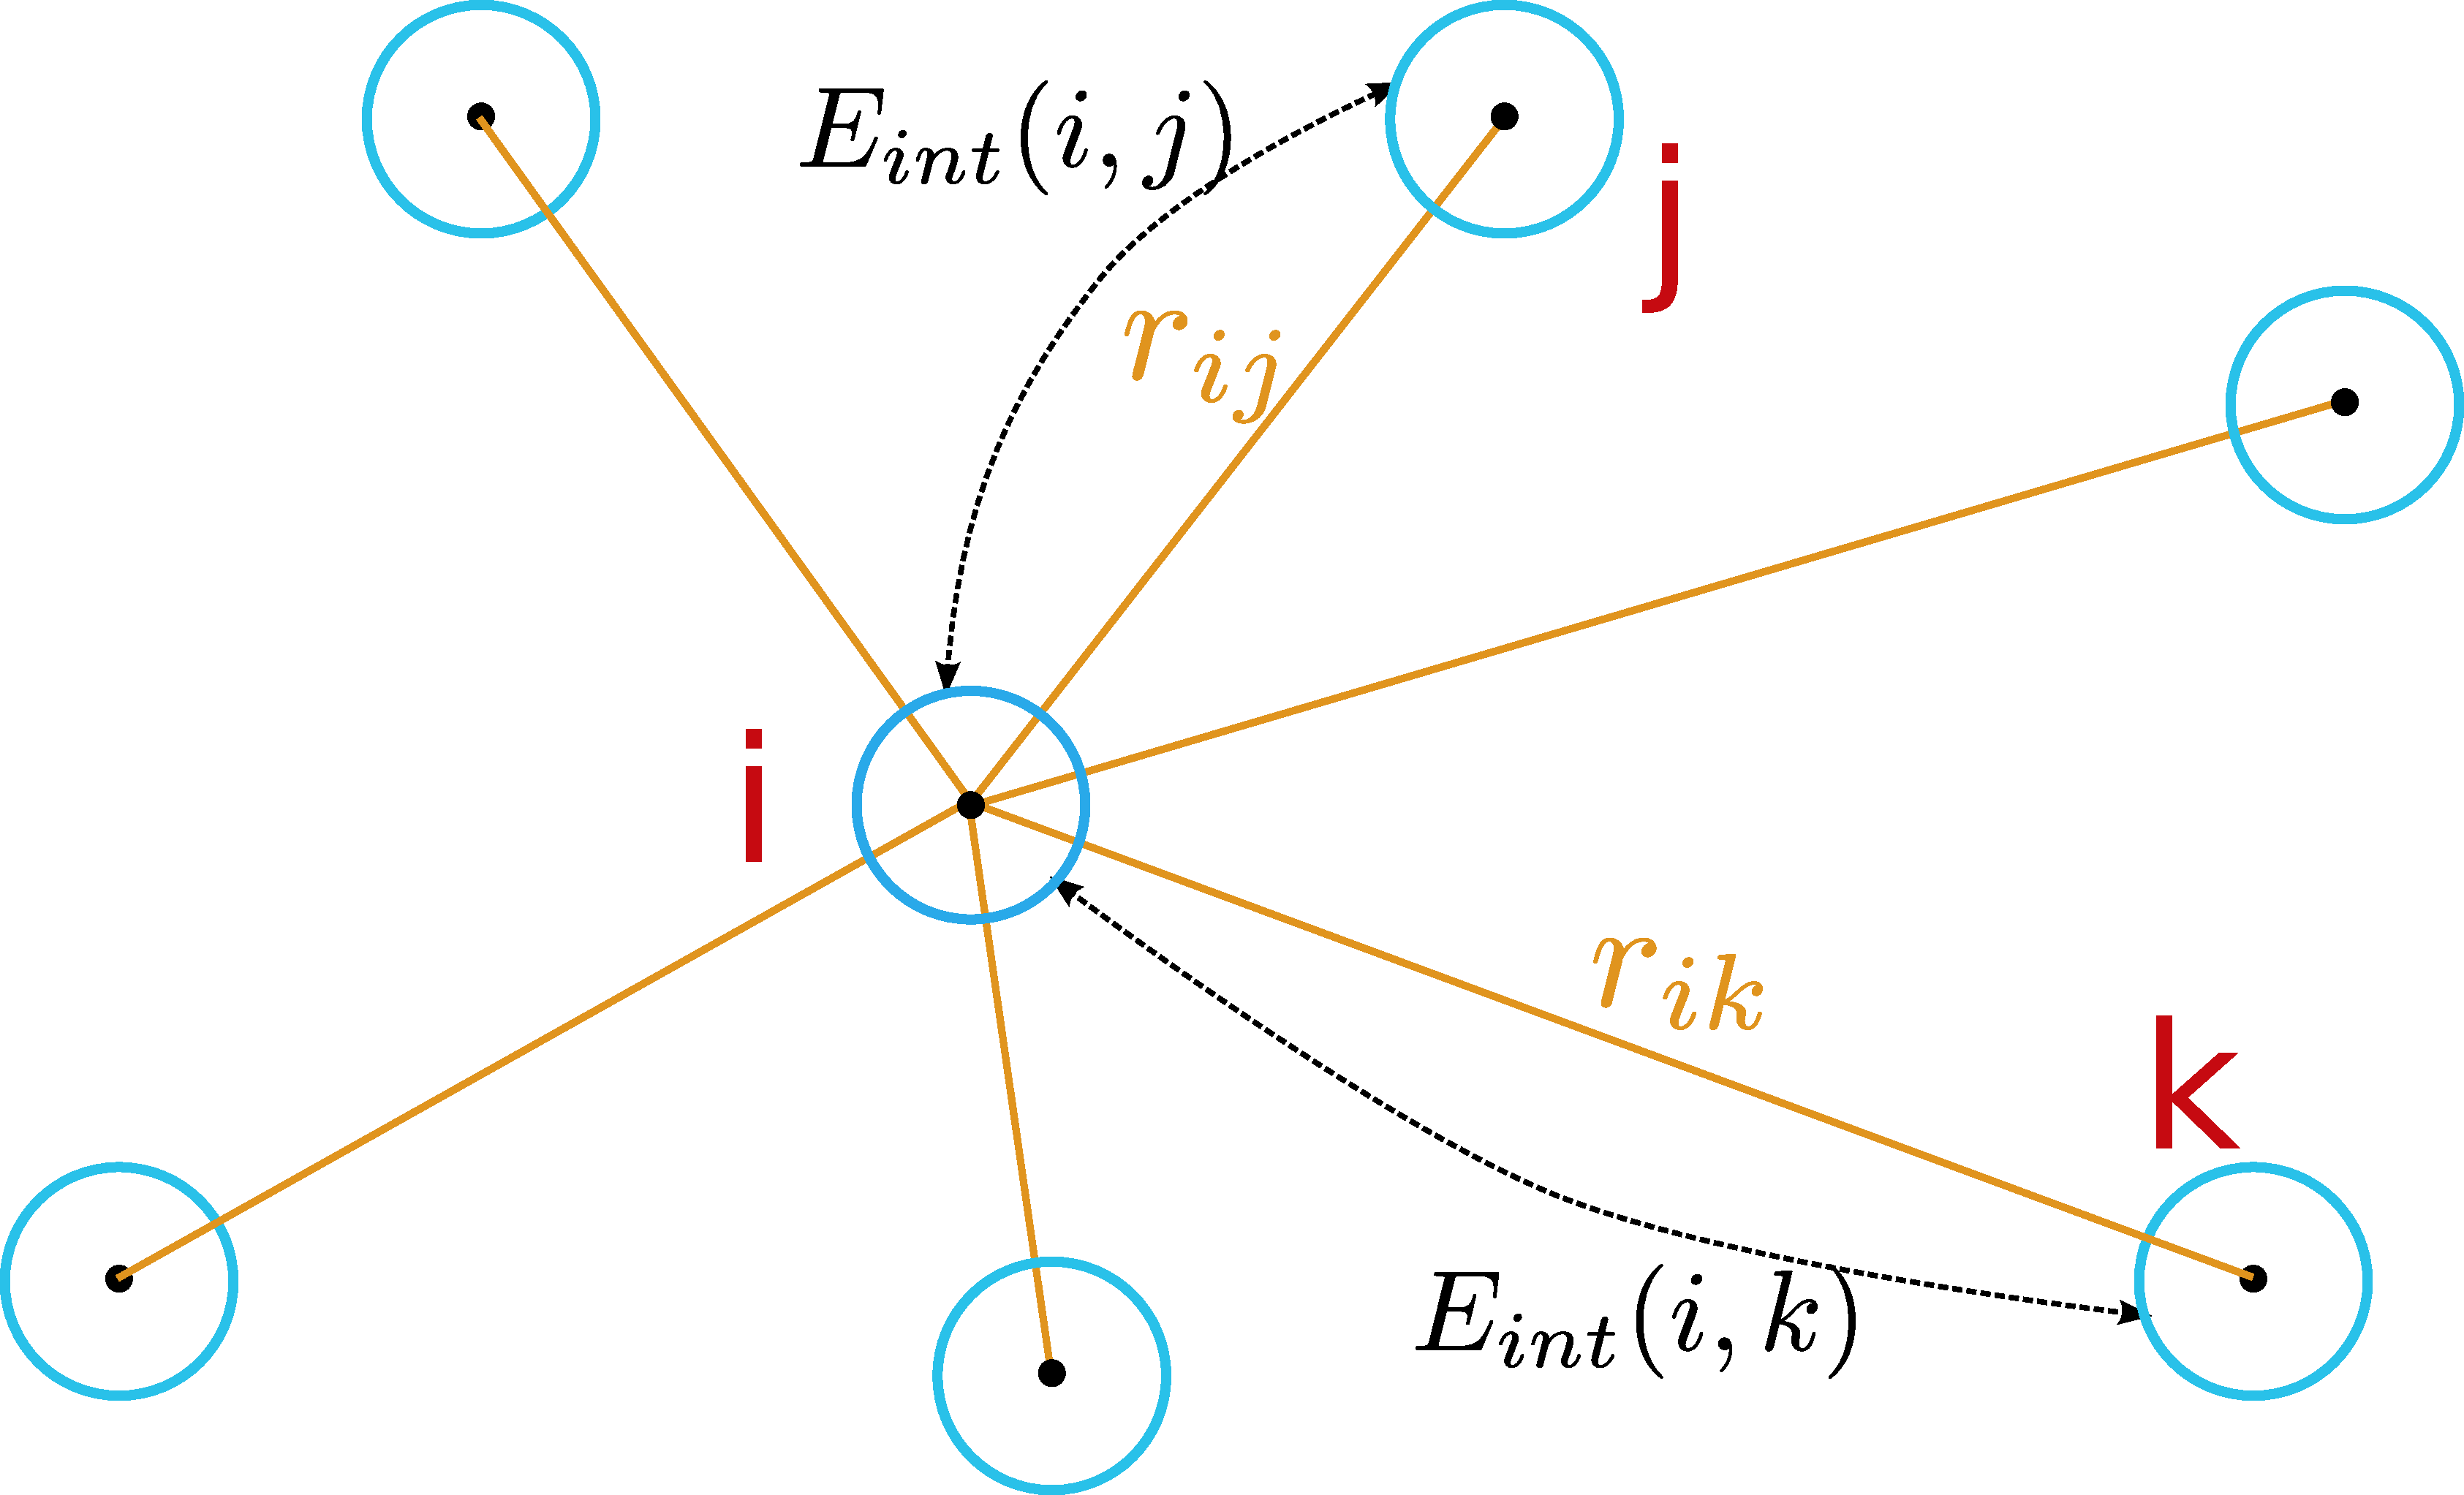
\includegraphics[width=0.6\linewidth]{figures/low_l/Natomes}
\caption[Ensemble de $N$ atomes de Rydberg en interaction van der Waals]
{Ensemble de $N$ atomes de Rydberg en interaction van der Waals.
L'énergie d'interaction de chaque atome est la somme de ses énergies d'interaction de paire avec tous les autres.
}
\label{fig:VdW_sum_N}
\end{figure}

	\subsection{Deux régimes d'excitation en interaction dipolaire forte}\label{subsec:excitation_bloc_facil}
	%Le blocage dipolaire et la facilitation}

\noindent Les interactions dipolaires ont une influence importante sur l'excitation d'un ensemble dense d'atomes de Rydberg.	
En effet, la présence d'un atome de Rydberg conditionne l'excitation ultérieure d'autres atomes de Rydberg dans son voisinage.
Lorsque l'excitation est faite à résonance, cet effet est connu sous le nom de \og blocage dipolaire \fg{}.

	\subsubsection*{Blocage dipolaire et super-atomes}
\noindent Le mécanisme du blocage dipolaire est illustré en figure (\ref{fig:dip_block} a)).
Considérons deux atomes dans l'état fondamental $\ket{g}$, séparés d'une distance $r$.
L'état de la paire est alors $\ket{g,g}$.
Un laser est accordé à résonance pour exciter l'un quelconque de ces deux atomes vers le niveau de Rydberg $\ket{Ry}$.
L'état de la paire devient ainsi $\ket{g,Ry}$. % ou $\ket{Ry,g}$.
Si l'on souhaite exciter le second atome vers le niveau $\ket{Ry}$, alors il faut considérer l'énergie nécessaire à la transition $\ket{g,Ry} \rightarrow \ket{Ry,Ry}$.
Or ce dernier état de paire subit un déplacement d'énergie dû à l'interaction de van der Waals
%
\begin{equation}
\label{eq:DeltaE_block}
\Delta E_{\ket{Ry,Ry}}(r) = E_{\ket{Ry,Ry}}(r)-E_{\ket{Ry,Ry}}(\infty)
= E_{int}(r).
\end{equation}
%
Le laser, qui était à résonance avec la transition $\ket{g,g}\rightarrow\ket{g,Ry}$, n'est ainsi plus à résonance avec la transition $\ket{g,Ry}\rightarrow\ket{Ry,Ry}$.
L'excitation du second atome vers un niveau de Rydberg s'en trouve bloquée.

\begin{figure}[!h]
\centering
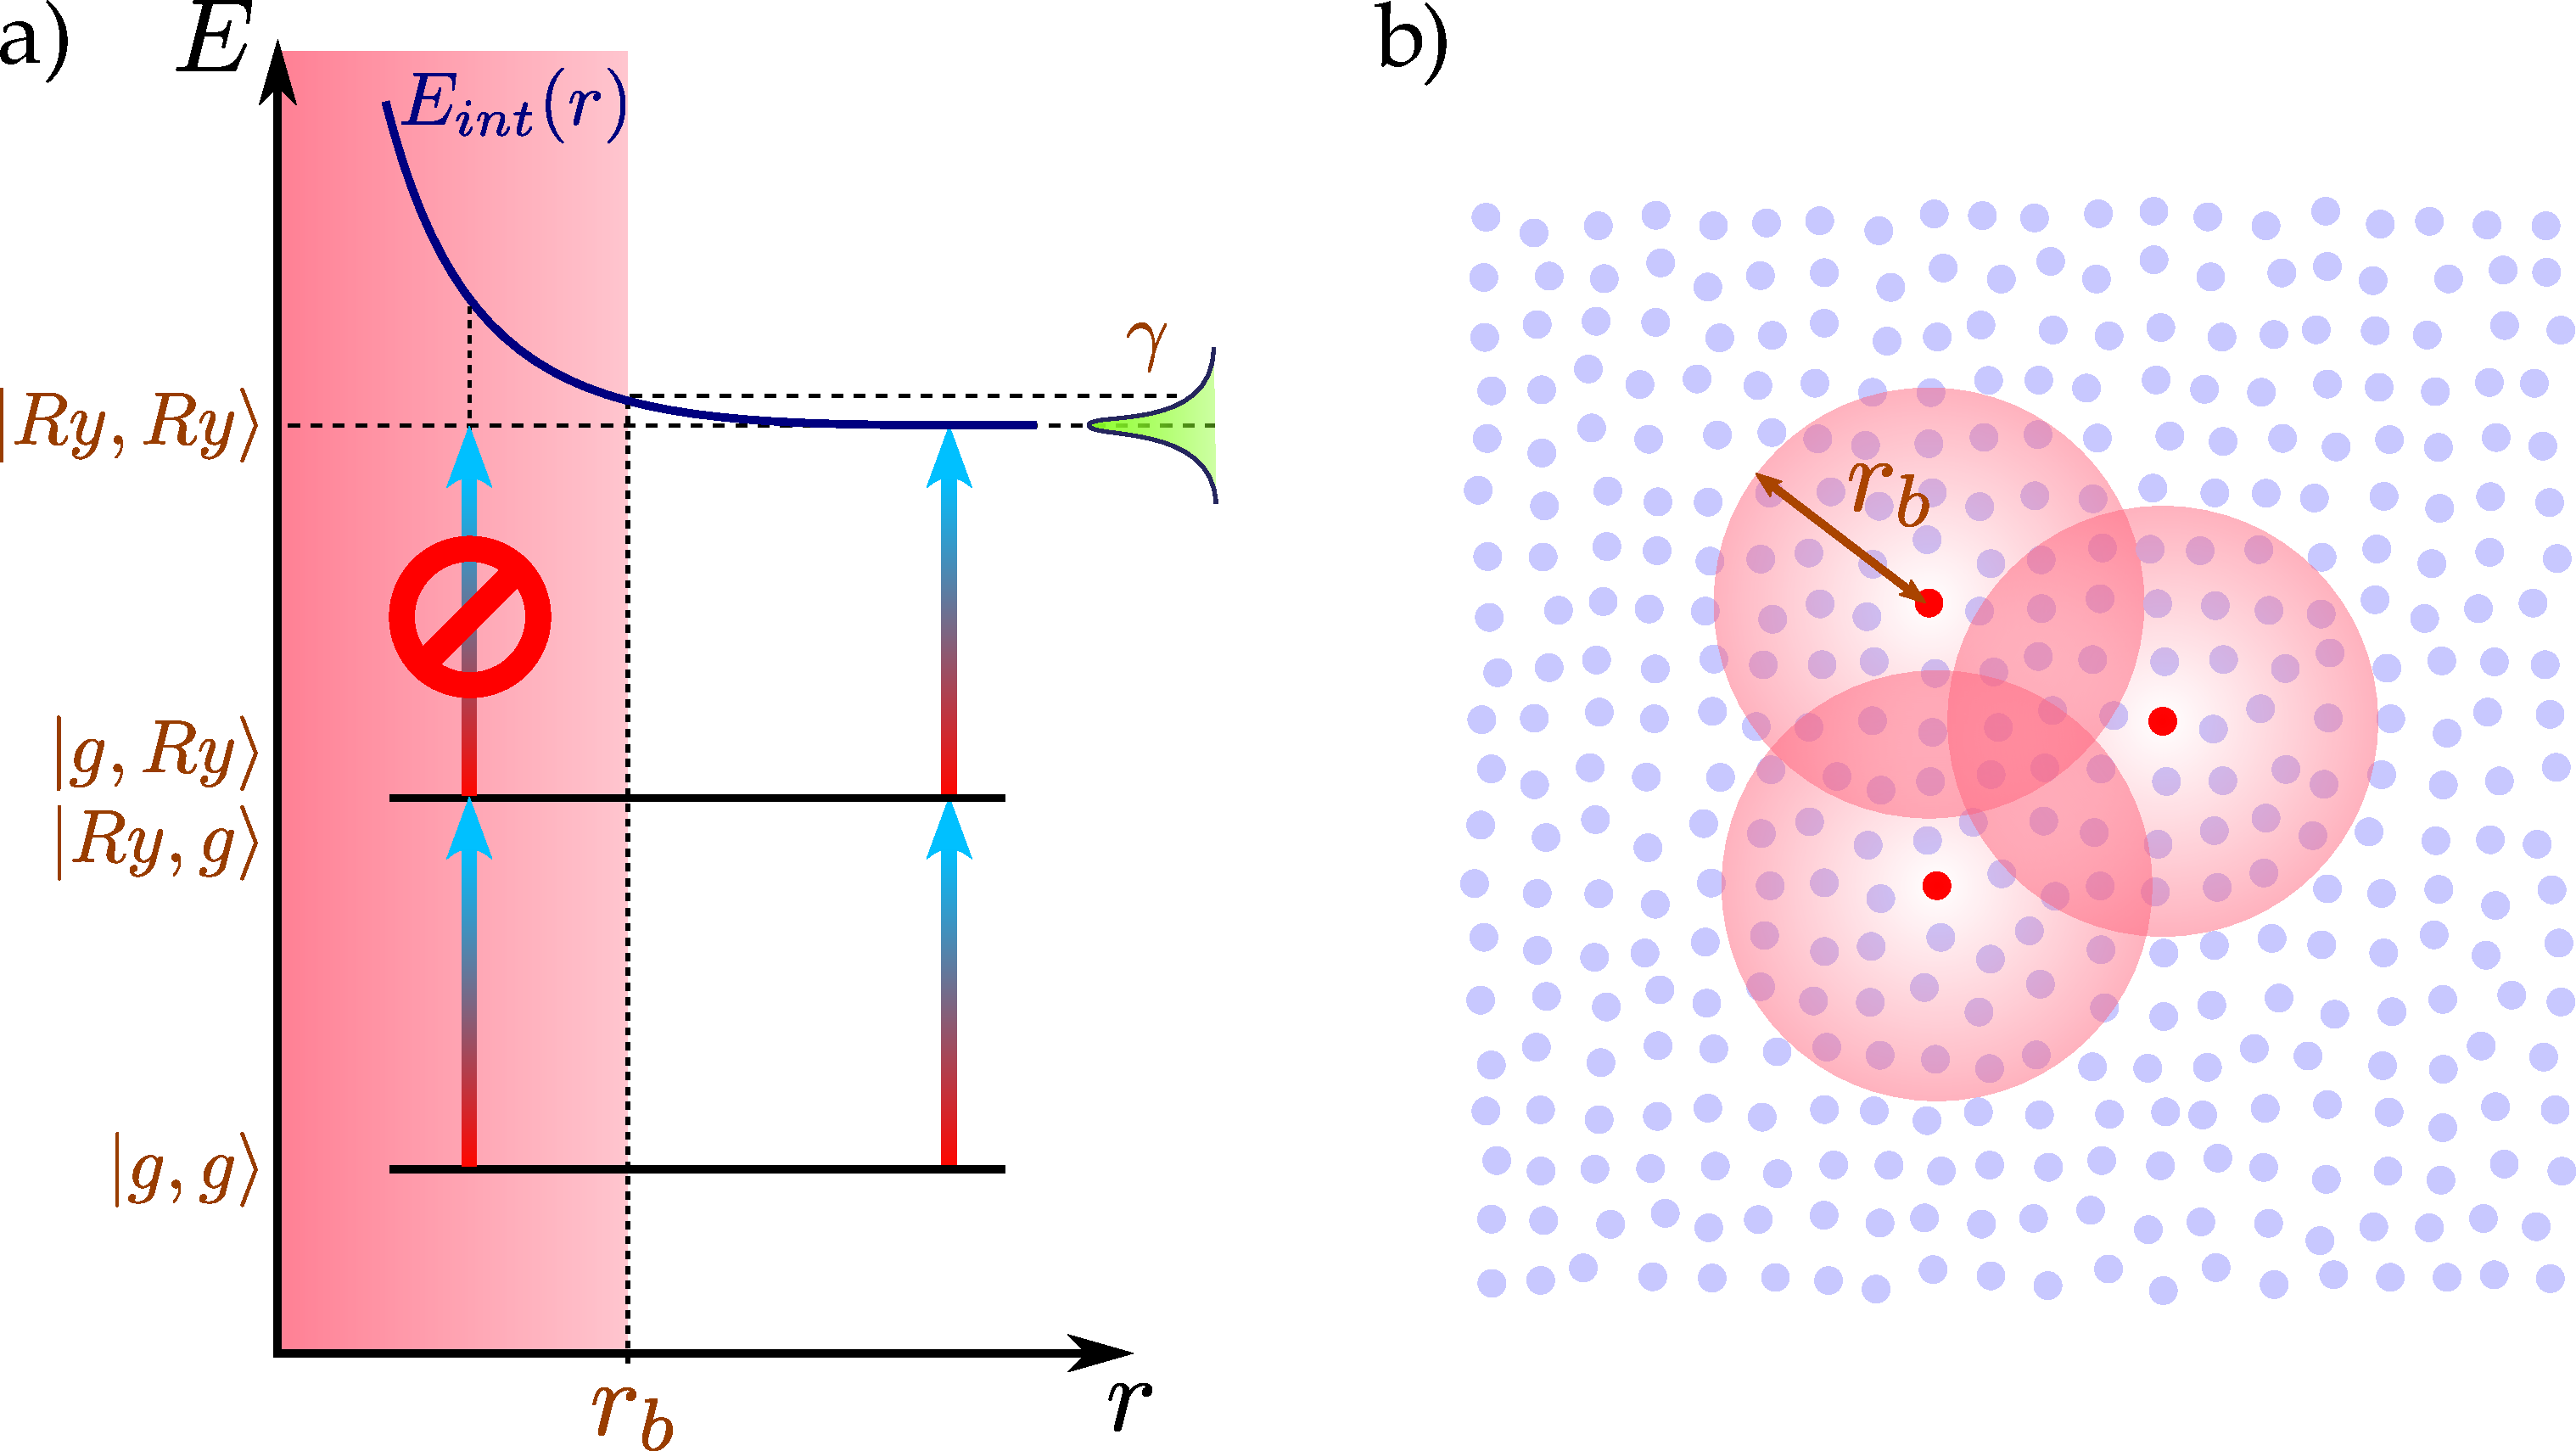
\includegraphics[height=.3\textheight]{figures/low_l/dip_block}
\caption[Mécanisme du blocage dipolaire]{
Illustration du mécanisme de blocage dipolaire.
\textbf{a)} Diagramme d'énergie des niveaux de paire à zéro, un ou deux atomes excités, en fonction de la distance interatomique $r$.
$\ket{g}$ est le niveau fondamental et $\ket{Ry}$ le niveau de Rydberg considéré.
Aux courtes distances, l'interaction dipolaire déplace l'excitation du deuxième atome vers le niveau de Rydberg hors de résonance avec le laser ayant excité le premier atome.
Les grandeurs $\gamma$, $E_{int}$ et $r_b$ représentent respectivement la largeur spectrale de la raie d'excitation à un atome, l'énergie d'interaction entre deux atomes de Rydberg et le \og rayon de blocage \fg{}.
\textbf{b)} Généralisation à un ensemble d'atomes. Les points bleu clair sont des atomes dans l'état fondamental et les points rouges sont des atomes de Rydberg.
Le mécanisme de blocage empêche l'excitation de deux atomes de Rydberg dans un même sphère de rayon $r_b$, représentée par les disques rouges.
}
\label{fig:dip_block}
\end{figure}

%Le laser d'excitation n'est pas infiniment fin spectralement et l'effet de blocage dipolaire sera limité par sa largeur spectrale.
La transition n'est pas infiniment fine spectralement et l'effet de blocage dipolaire sera limité par sa largeur spectrale $\gamma$, dominée en pratique par la largeur du laser.
On peut en effet considérer que le laser est résonant avec la transition dès lors que le désaccord entre eux est inférieur à la demi-largeur spectrale $\gamma/2$ de la raie d'excitation.
Nous définissons ainsi le \og rayon de blocage \fg{} $r_b$ comme étant la distance en-deçà de laquelle le désaccord est supérieur à la demi-largeur spectrale :
\begin{equation}
\label{eq:def_condit_bloc}
\Delta E_{int}(r_b) = \gamma /2 .
\end{equation}
%
Dans le cas qui nous intéresse, l'interaction dipolaire a une forme de van der Waals en $1/^6$, permettant de réécrire l'équation \eqref{eq:def_condit_bloc} sous la forme
\begin{equation}
\label{eq:def_rayon_bloc}
\frac{C_6}{r^6} = \gamma /2 \text{ , soit } r_b = \sqrt[6]{\frac{C_6}{\gamma /2}} .
\end{equation}
%
Le mécanisme de blocage est donc effectif à l'intérieur d'un \og volume de blocage\fg{} autour de chaque atome de Rydberg déjà excité.
Ce volume de blocage est une sphère de rayon $r_b$, représentée en figure (\ref{fig:dip_block} b)).

Revenons au cas de deux atomes :
il existe deux états de paire à une excitation, qui sont $\ket{g,Ry}$ et $\ket{Ry,g}$.
Ces deux états sont dégénérés et le laser couple le niveau fondamental $\ket{g,g}$ indifféremment à $\ket{g,Ry}$ et à $\ket{Ry,g}$, avec une même fréquence de Rabi $\Omega$.
La combinaison symétrique $\ket{D} = \left( \ket{g,Ry} + \ket{Ry,g} \right) / \sqrt{2}$, appelée état collectif de Dicke des deux atomes, est alors couplée à l'état fondamental avec une fréquence de Rabi augmentée $\Omega\sqrt{2}$.
Ce facteur d'accroissement a été mis en évidence expérimentalement par le groupe de A. Browaeys et P. Grangier \cite{MX_BROWAEYS_COLLECRABIBLOCK}, en observant deux atomes piégés dans des pinces optiques.
La combinaison antisymétrique $\left( \ket{g,Ry} - \ket{Ry,g} \right) / \sqrt{2}$ n'est quant à elle pas couplée au niveau fondamental par l'excitation.

L'idée se généralise au cas à $N$ atomes en utilisant encore une fois le modèle de Dicke.
Dans un rayon de blocage contenant $N_b$ atomes, l'état du système oscille entre l'état fondamental et l'état de Dicke à une excitation, toute excitation supplémentaire étant interdite par blocage dipolaire.
Cette oscillation se fait cette fois avec une fréquence de Rabi $\Omega\sqrt{N_b}$.
Un modèle simple de ce phénomène consiste à voir l'ensemble de ces $N_b$ atomes comme un unique \og super-atome \fg{} ayant un moment de transition dipolaire $\sqrt{N_b}$ plus grand  que celui d'un atome isolé.
Ce modèle de super-atome a été exploité avec succès pour expliquer des observations expérimentales par les groupes d'I. Bloch \cite{MX_BLOCH_SUPERATOM} et de H. Ott \cite{MX_OTT_SUPERATOM}.


	\subsubsection*{Excitation facilitée et agrégats de Rydberg}
	
\noindent Dans le régime de blocage dipolaire, l'interaction entre atomes de Rydberg désaccorde toute excitation supplémentaire au voisinage d'un premier atome de Rydberg.
On peut alors imaginer décaler la fréquence du laser d'excitation de façon à compenser ce désaccord et ainsi retrouver une condition de résonance.

Reprenons le cas de deux atomes présenté ci-dessus en figure \eqref{fig:dip_block}.
Considérons cette fois un laser désaccordé de $\Delta$ par rapport à la transition $\ket{g,g} \rightarrow \ket{g,Ry}$, tel que représenté en figure \eqref{fig:dip_facil}.
Le premier atome pourra toujours être excité hors résonance par le laser désaccordé.
Le second atome sera ensuite excité, à résonance, si la condition
%
\begin{equation}
\label{eq:condition_facil}
\Delta = E_{int}(r)/h = \frac{C_6}{r^6} > 0
\end{equation}
%
est satisfaite.
\`A un désaccord laser $\Delta$ fixé correspond ainsi un \og rayon de facilitation \fg{}, défini par
%
\begin{equation}
\label{eq:r_facil}
r_f = \sqrt[6]{\frac{C_6}{\Delta}}.
\end{equation}
%
L'excitation du second atome de Rydbegr est donc \og facilitée \fg{} par la présence du premier.
%En raison de la largeur spectrale $\gamma$ du laser, l'excitation du second atome de Rydberg est donc \og facilitée \fg{} par la présence du premier, 
En tenant compte de la largeur $\gamma$ de la raie d'excitation, la condition de facilitation est obtenue dès lors que les deux atomes sont séparés d'une distance $r_f \pm \delta r_f$,
où %$\delta r_f = \frac{1}{2} \left( \sqrt[6]{C_6/(\Delta-\gamma/2)} - \sqrt[6]{C_6/(\Delta+\gamma/2)} \right)$, soit 
$\delta r_f \simeq r_f \gamma / (12\Delta)$ au premier ordre en $\gamma / \Delta$.
La figure (\ref{fig:dip_facil} a) représente ce mécanisme d'\og excitation facilitée \fg{} .
%	
\begin{figure}[!h]
\centering
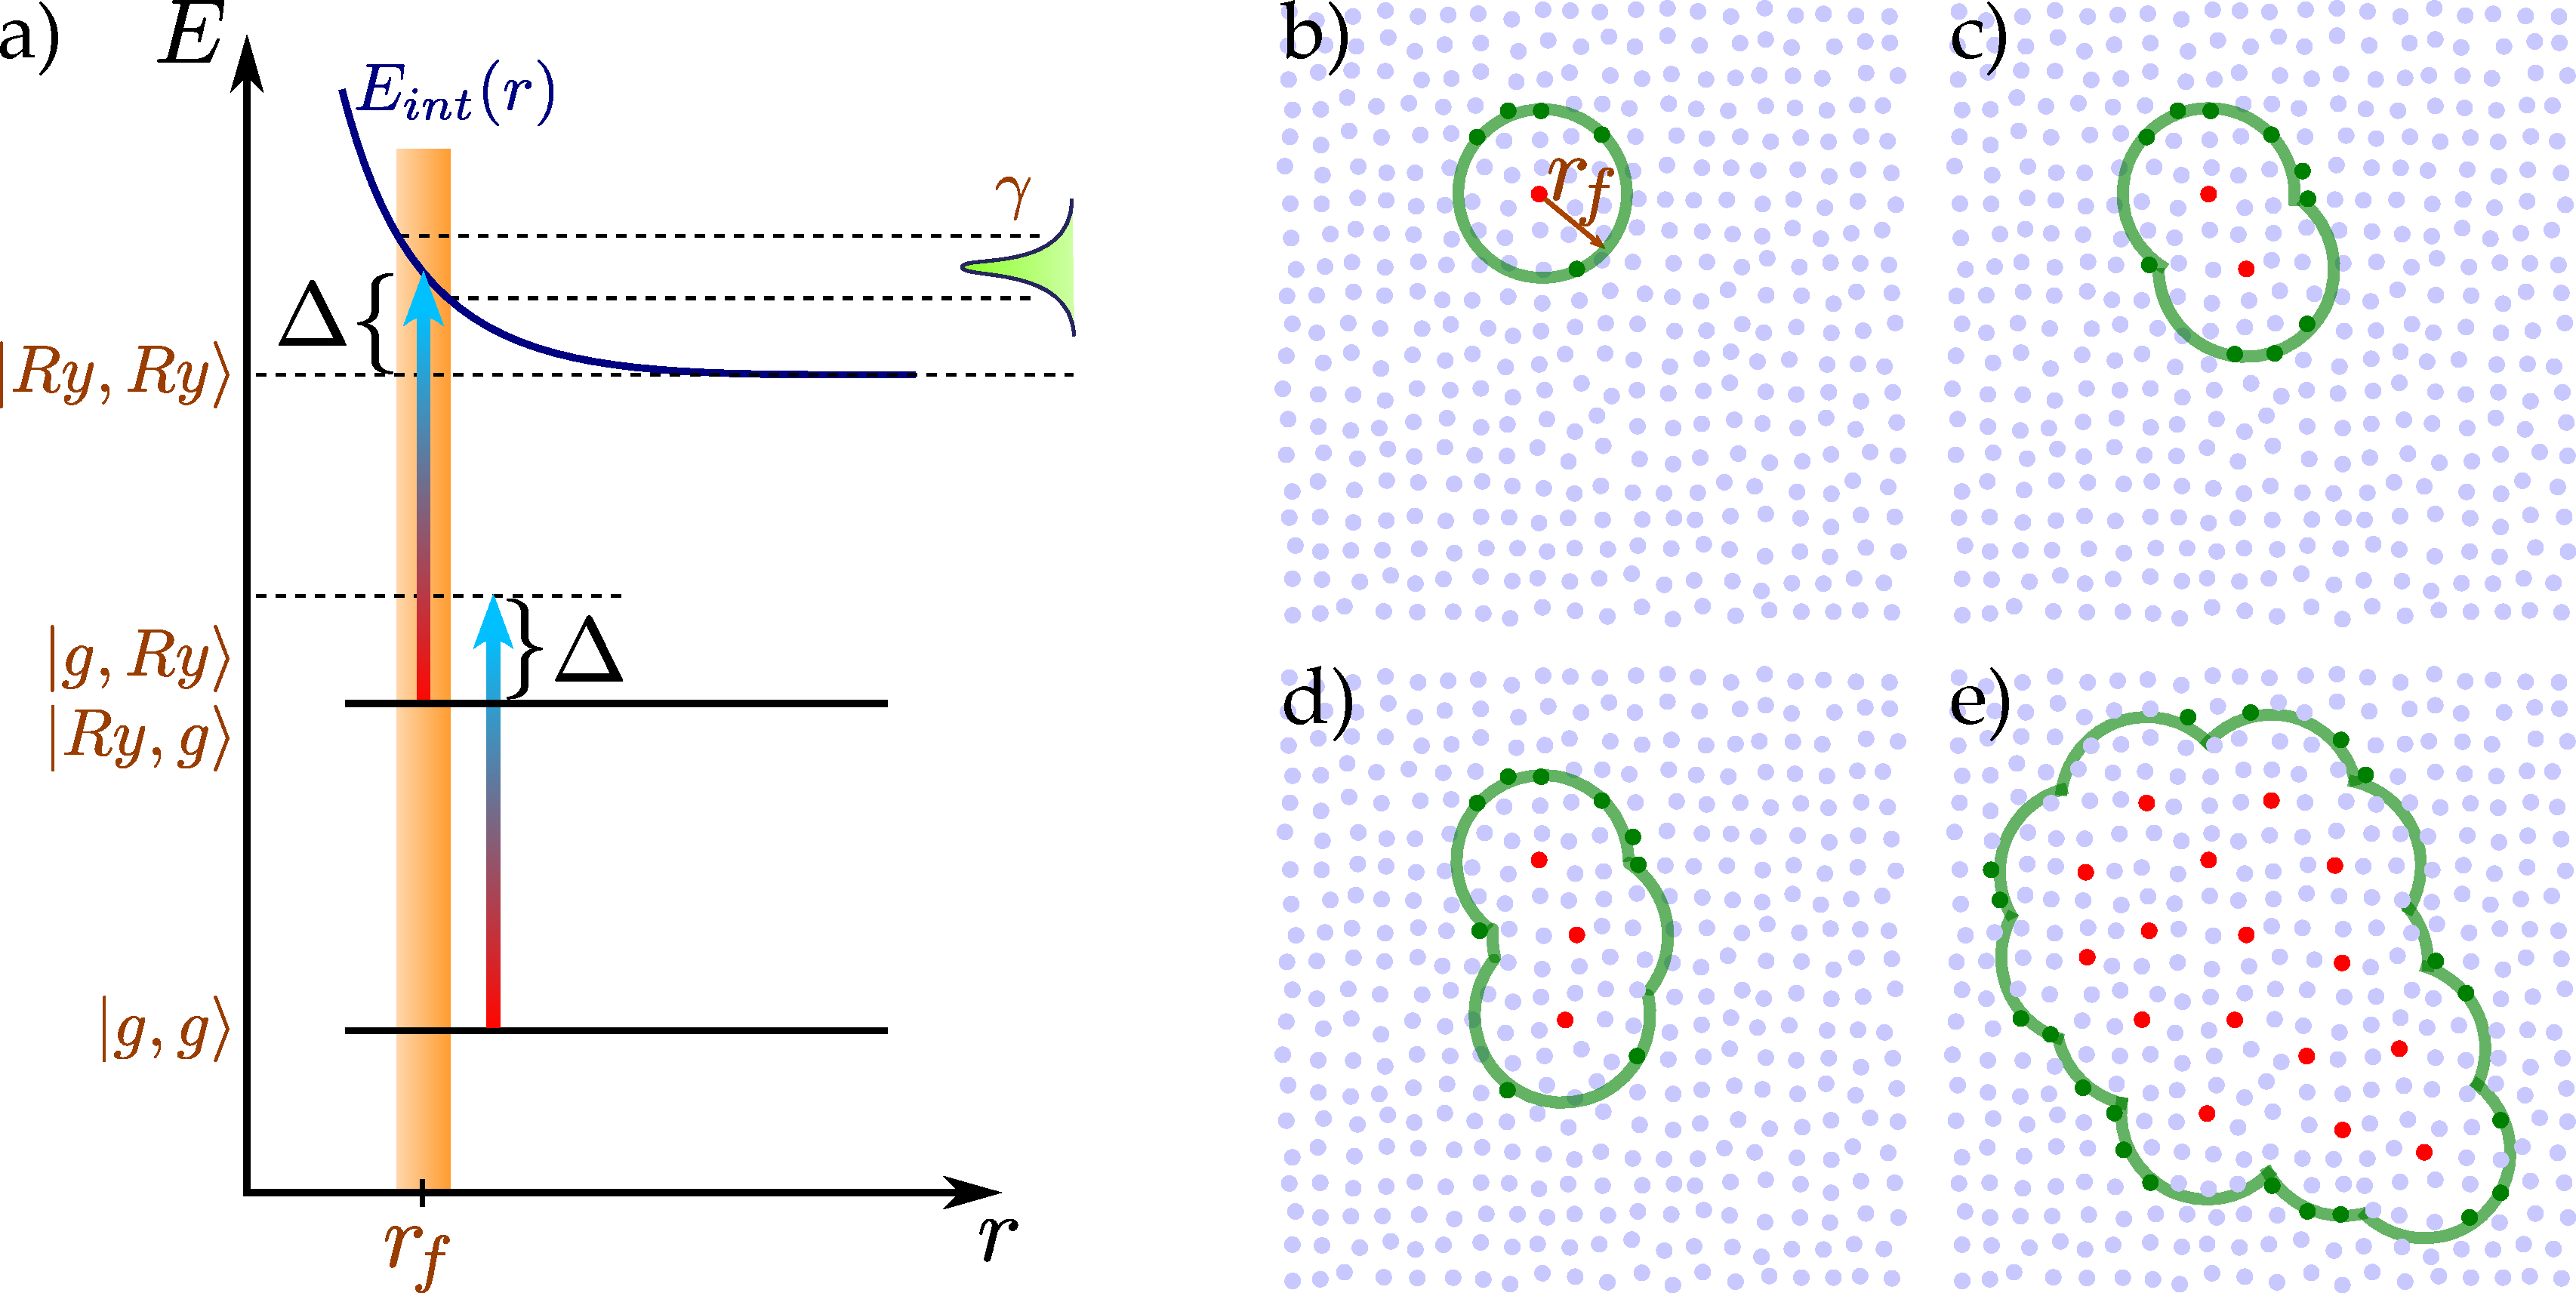
\includegraphics[height=.3\textheight]{figures/low_l/dip_facil}
\caption[Mécanisme de d'excitation facilitée]{
Mécanisme de d'excitation facilitée.
\textbf{a)} Diagramme d'énergie des niveaux de paire à zéro, une ou deux atomes excités, en fonction de la distance interatomique $r$.
Le premier atome de Rydberg est excité hors résonance.
Le désaccord $\Delta$ du laser permet de compenser l'interaction dipolaire à la distance $r_f$ et d'exciter à résonance le second atome.
\textbf{b) - e)} Évolution dans le temps d'un agrégat de Rydberg.
Les points bleu clair représentent l'ensemble de départ d'atomes dans l'état fondamental et les points rouges représentent les atomes de Rydberg.
Les bandes vertes représentent les régions \og facilitées \fg{} définies par l'équation \eqref{eq:facil_Natomes} où de nouveaux atomes de Rydberg peuvent être excités à résonance.
}
\label{fig:dip_facil}
\end{figure}

Au sein d'un ensemble d'atomes, chacun a une probabilité égale d'être le premier atome excité, hors résonance, vers un niveau de Rydberg.
Dès lors que ce premier atome de Rydberg est excité, l'excitation est facilitée pour les atomes qui sont à une distance $r_f$ de celui-ci, vérifiant par-là la condition \eqref{eq:r_facil}.
L'excitation facilitée continue ainsi de proche en proche, tant qu'il existe un atome $i$ satisfaisant
\begin{equation}
\label{eq:facil_Natomes}
\Delta = \sum_{j\neq i} {\frac{C_6}{r_{ij}^6}},
\end{equation}
où la somme est faite sur tous les atomes de Rydberg $j$ déjà excités, situés chacun à distance $r_{ij}$ de l'atome $i$.

Le phénomène de blocage dipolaire est remplacé ici par la formation rapide d'un \og agrégat de Rydberg \fg{} fortement corrélé, autour du premer atome de Rydberg, la \og graine \fg{} de cet agrégat.
Les distances relatives entre atomes de Rydberg sont déterminées par l'équation \eqref{eq:facil_Natomes} et donc contrôlées par le désaccord $\Delta$ du laser d'excitation.
Les figures (\ref{fig:dip_facil} b)-e)) représentent cette excitation séquentielle facilitée d'un agrégat de Rydberg.

\newpage
	\subsection{Mouvement des atomes au sein d'un gaz dense de Rydberg}
	\noindent Le second effet des interactions dipolaires au sein d'un nuage d'atomes de Rydberg est un effet mécanique.
Comme nous l'avons vu en \ref{sec:interacting_rydbergs}, l'interaction est répulsive entre atomes de Rydberg dans le même niveau $\ket{\mathrm{nS}}$.
Ainsi, deux atomes de Rydberg en interaction dipolaire subiront chacun une force répulsive, directement dérivée de leur énergie d'interaction,
\begin{equation}
\label{eq:repuls_2atoms}
F = - \frac{d E_{int}}{dr}  = + \frac{6hC_6}{r^7}.
\end{equation}
Cela équivaut à un traitement classique de l'effet mécanique de l'interaction dipolaire, bien que le calcul de cette même interaction ne le soit pas.
Cela est permis par la forme de l'interaction dipolaire entre deux atomes dans le même état de Rydberg, donnée par l'équation \eqref{eq:Vdd_aa}, qui consiste en un simple déplacement d'énergie du niveau de paire $\ket{Ry,Ry}$.

Prenons l'exemple de deux atomes dans le niveau $\mathrm{60S}$, séparés d'une distance de $\SI{5}{\um}$ : leur énergie d'interaction vaut $hC_6/r^6 = h\cdot {\SI{137.6}{\GHz\raiseto{6}\um}}/(\SI{5}{\um})^6 = h\times\SI{8.8}{\MHz}$.
Ils se repoussent donc avec une force valant %$6hC_6/r^7 = 6h\cdot \SI{137.6}{\GHz\raiseto{6}\um}/(\SI{5}{\um})^7 = \SI{6.97e-27}{\mega\newton} = \SI{6.97e-21}{\newton}$.
$6hC_6/r^7 =\SI{6.97e-21}{\newton}$.
Étant donnée la masse du rubidium, cette force répulsive correspond à une accélération valant $F/m_{Rb87} = \SI{4.83e4}{\m\per\s\squared}$, soit $\num{5000}$ fois plus que l'accélération de la gravité.
Une intégration numérique grossière permet d'extraire un ordre de grandeur du déplacement des atomes : en $\SI{20}{\us}$, ils auront presque atteint leur vitesse relative maximale de $\SI{0.284}{\m\per\s}$ et en $\SI{10}{\us}$ seulement la distance qui les sépare aura augmenté de $\SI{1.75}{\um}$.
Leur énergie d'interaction aura par là chuté d'un facteur $\SI{5.77}{}$, ce qui constitue une modification considérable de l'interaction.

La généralisation à $N$ atomes se fait en additionnant vectoriellement les forces répulsives dues à chaque interaction de paire :
\begin{equation}
\label{eq:repuls_Natomes}
\vec{F}(i) =  \sum_{j\neq i} -\vec{\nabla}E_{int}(i,j)
= \sum_{j\neq i} \frac{6hC_6}{r_{ij}^7} \cdot \frac{-\vec{r}_{ij}}{r_{ij}}
= - 6hC_6 \cdot \sum_{j\neq i} \frac{\vec{r}_{ij}}{r_{ij}^8}.
\end{equation}
%
Cette force répulsive décroît très vite avec la distance.
Le traitement ci-dessus du cas de deux atomes atteste que
%On s'attend ainsi à ce que deux atomes de Rydberg en interaction 
ceux-ci s'accélèrent mutuellement pendant un temps court, se propageant ensuite balistiquement dans des directions opposées.
%C'est ce que confirme l'exemple de la paire $\ket{\mathrm{60S,60S}}$ précédemment cité.
Il est intéressant de noter qu'au sein d'un nuage de nombreux atomes de Rydberg, les atomes du c\oe ur  sont repoussés par les interactions dipolaires de tous les côtés.
Les atomes du bord du nuage seront alors expulsés en premier, puis petit à petit les atomes plus au centre pourront commencer à se déplacer.
Le nuage subit ainsi une expansion hydrodynamique non triviale, que nous mesurerons expérimentalement et simulerons numériquement.

\clearpage
\section{Observation expérimentale des interactions}
\noindent Afin de mettre en évidence les effets des interactions dipolaires, nous avons mené deux expériences complémentaires.
En premier lieu, la spectroscopie optique du nuage permet de s'intéresser à l'excitation sous blocage dipolaire fort et à l'excitation facilitée à désaccord positif.
Ensuite, la spectroscopie microonde du nuage, à différents délais après l'excitation laser, permet de sonder la distribution des énergies d'interaction au sein du nuage au cours de son expansion.
Ces expériences sont discutées en détail dans la thèse de Raul Celistrino Teixeira \cite{PHD_CELISTRINO}.

	\subsection{Spectroscopie optique du nuage : différents régimes d'excitation}\label{subsec:optical_spectra}
	\subsubsection*{Conditions de l'expérience}
\noindent	L'expérience de spectroscopie optique vise à observer l'excitation des atomes de Rydberg sous l'influence des interactions dipolaires, dans les régimes de blocage et d'excitation facilitée.
Cela nécessite, entre autres, un nuage d'atomes dans l'état fondamental suffisamment dense afin que la condition de facilitation \eqref{eq:facil_Natomes} puisse être satisfaite.
Cependant, une forte densité d'atomes dans l'état fondamental risque d'interférer avec l'excitation de Rydberg, indépendamment des interactions dipolaires.
En effet, l'électron de Rydberg, qui est presque libre, est sensible à cette densité atomique.
En première approximation, l'interaction entre l'électron de Rydberg et les atomes dans l'état fondamental prend la forme d'un déplacement d'énergie $V_e$ proportionnel à la densité atomique moyenne $\bar{\rho}$ \cite{MX_PFAURYDBERGBEC13} :
\begin{equation}
\label{eq:Pfau_shift}
V_e = \frac{2\pi \hbar ^2 a_s}{m_e} \bar{\rho},
\end{equation}
où $a_s$ est la longueur de diffusion caractérisant la force de l'interaction.
Le groupe de T. Pfau a mis en évidence cette interaction et obtenu une longueur de diffusion pour le \Rb{87} valant $a_s = -\SI{16.1}{}~a_0~$, indépendante du nombre quantique principal $n$ \cite{MX_PFAURYDBERGBEC13}.
%Le potentiel d'interaction $V_e$ étant négatif, nous avons ici affaire à une interaction qui abaisse l'énergie des niveaux de Rydberg.
Dans un condensat de Bose-Einstein avec une densité atomique typique de $\SI{e13}{\per \raiseto{3}\centi\meter}$, l'énergie d'interaction est de l'ordre de $V_e/h = -\SI{1}{\MHz}$.
%Dans ce cas, nous serions en présence de deux interactions antagonistes de même ordre de grandeur : l'interaction dipôle-dipôle répulsive, qui augmente l'énergie des niveaux de Rydberg et l'interaction de l'électron de Rydberg avec les atomes dans l'état fondamental, qui abaisse l'énergie des niveaux de Rydberg.
Les profils gaussiens de densité atomique avec lesquels nous travaillons causeraient alors un élargissement inhomogène de la raie spectrale d'excitation d'un seul atome de Rydberg.
Cela aurait pour effet de réduire le rayon de blocage, qui dépend directement de la largeur spectrale de l'excitation sans interaction dipolaire.

Il nous a fallu trouver une densité atomique permettant l'observation de l'excitation facilitée et du blocage dipolaire, tout en limitant l'effet d'interaction de l'électron de Rydberg avec les atomes dans l'état fondamental.
La spectroscopie optique de l'excitation de Rydberg a été faite dans un nuage thermique froid proche de la dégénérescence et non dans un condensat de Bose Einstein.
Ce nuage comporte $\SI{12000}{} \pm \SI{1000}{}$ atomes, piégés magnétiquement à environ $\SI{210}{\um}$ de la puce atomique.
Le piège prend une forme très allongée dans la direction $x$ de propagation des lasers et les atomes sont refroidis à une température de $\SI{600}{} \pm \SI{300}{\nano\kelvin}$.
Le profil de densité atomique est alors gaussien dans les trois directions, avec des rayons à $e^{-1/2}$ valant respectivement $(\sigma_x;\sigma_y;\sigma_z) = (\num{23.2} ; \num{4.5} ; \num{4.2})\si{\um}$.
La densité au centre vaut ici $n_0 = (\num{1.7}\pm\SI{0.15}{})\cdot \SI{e12}{\per\raiseto{3}\cm}$.
Cela limite l'interaction de l'électron de Rydberg avec les atomes dans l'état fondamental à une énergie $V_e = -h\times\SI{168}{\kHz}$, très inférieure à la largeur spectrale d'excitation à un atome, estimée \footnote{
Cette valeur est extraite de l'ajustement gaussien d'un spectre d'excitation optique dans un piège dilué et à faible excitation, donc sans interactions dipolaires.
Ce spectre est présenté comme référence en figure \eqref{fig:data_spectresoptiques}.}
à $\gamma = \SI{626}{\kHz}$.
La contribution de cette interaction pourra ainsi être négligée dans la suite de notre discussion.


		\subsubsection*{Résultats expérimentaux}
\noindent Les spectres d'excitation du niveau de Rydberg $\mathrm{60S}$ depuis le niveau fondamental $\mathrm{5S}$, obtenus pour différentes durées d'impulsion laser, sont représentés en figure \eqref{fig:data_spectresoptiques}.
Le graphe représente aussi un spectre d'excitation dans un nuage dilué et à faible taux d'excitation, servant de spectre de référence sans interactions.
%
\begin{figure}[!h]
\centering
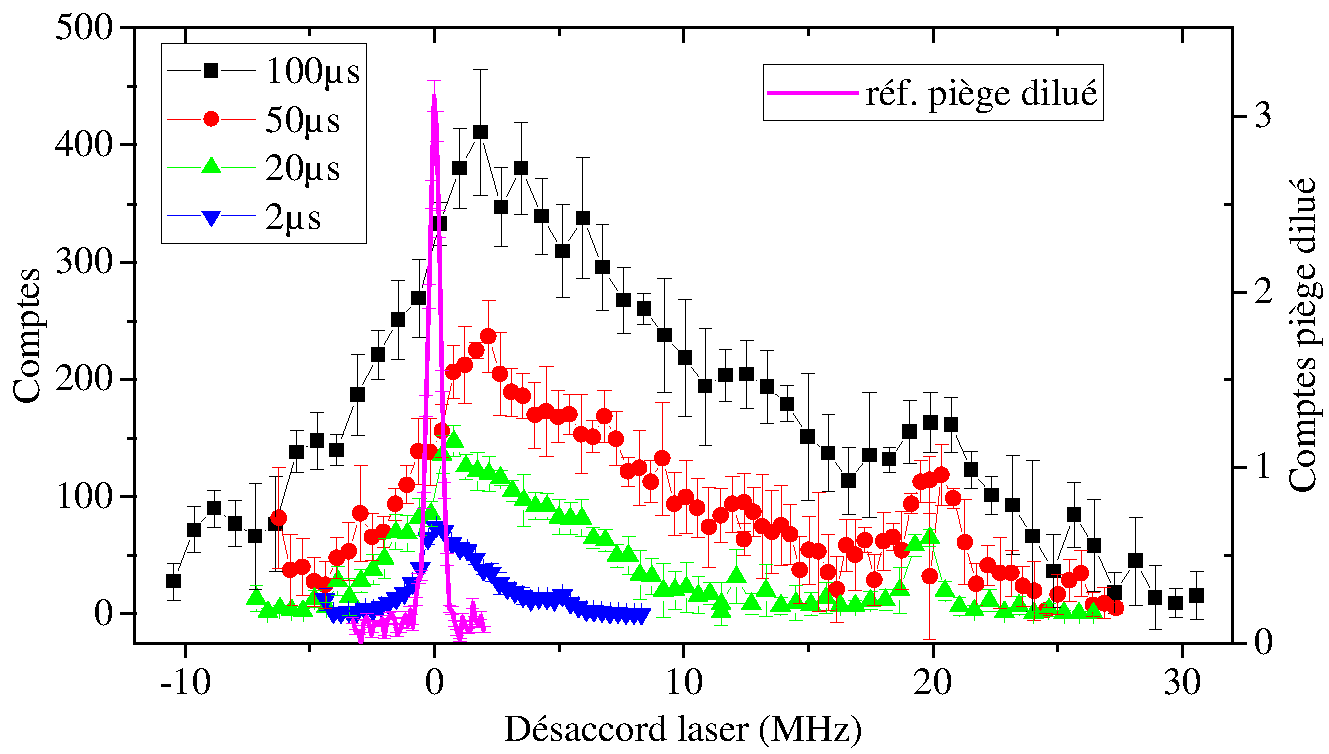
\includegraphics[width=\linewidth]{figures/low_l/data_spectres_optiques}
\caption[Spectres optiques d'excitation en régime d'interaction dipolaire forte]{Spectres optiques d'excitation en régime d'interaction dipolaire forte.
L'excitation est réalisée à différentes durées d'impulsion laser : $\SI{2}{}$, $\SI{20}{}$, $\SI{50}{}$ et $\SI{100}{\us}$.
La courbe magenta en trait plein est un spectre de référence sans interaction, représenté avec une échelle différente (échelle de droite).
Les pics d'excitation autour de $\Delta = \SI{20}{\MHz}$ sont dûs à la modulation en fréquence du laser, nécessaire à sa stabilisation par un dispositif Pound-Drever-Hall.
}
\label{fig:data_spectresoptiques}
\end{figure}
%
Un élargissement vers les hautes fréquences apparaît très clairement dès les faibles temps d'excitation.
Cet élargissement est caractéristique de l'excitation facilitée par interaction :
une fois le premier atome de Rydberg excité, un agrégat se forme rapidement autour et permet d'amplifier largement l'excitation à désaccord positif.
Plus le désaccord est élevé cependant, plus longtemps se fera attendre cette première excitation, ce qui explique l'élargissement de plus en plus prononcé aux temps d'impulsion longs.

Cela se voit très bien sur les graphes de la figure \eqref{fig:data_saturoptique}, qui représente l'évolution du nombre d'atomes de Rydberg excité en fonction de la durée d'impulsion laser, pour différents désaccords.
%
\begin{figure}[!h]
\centering
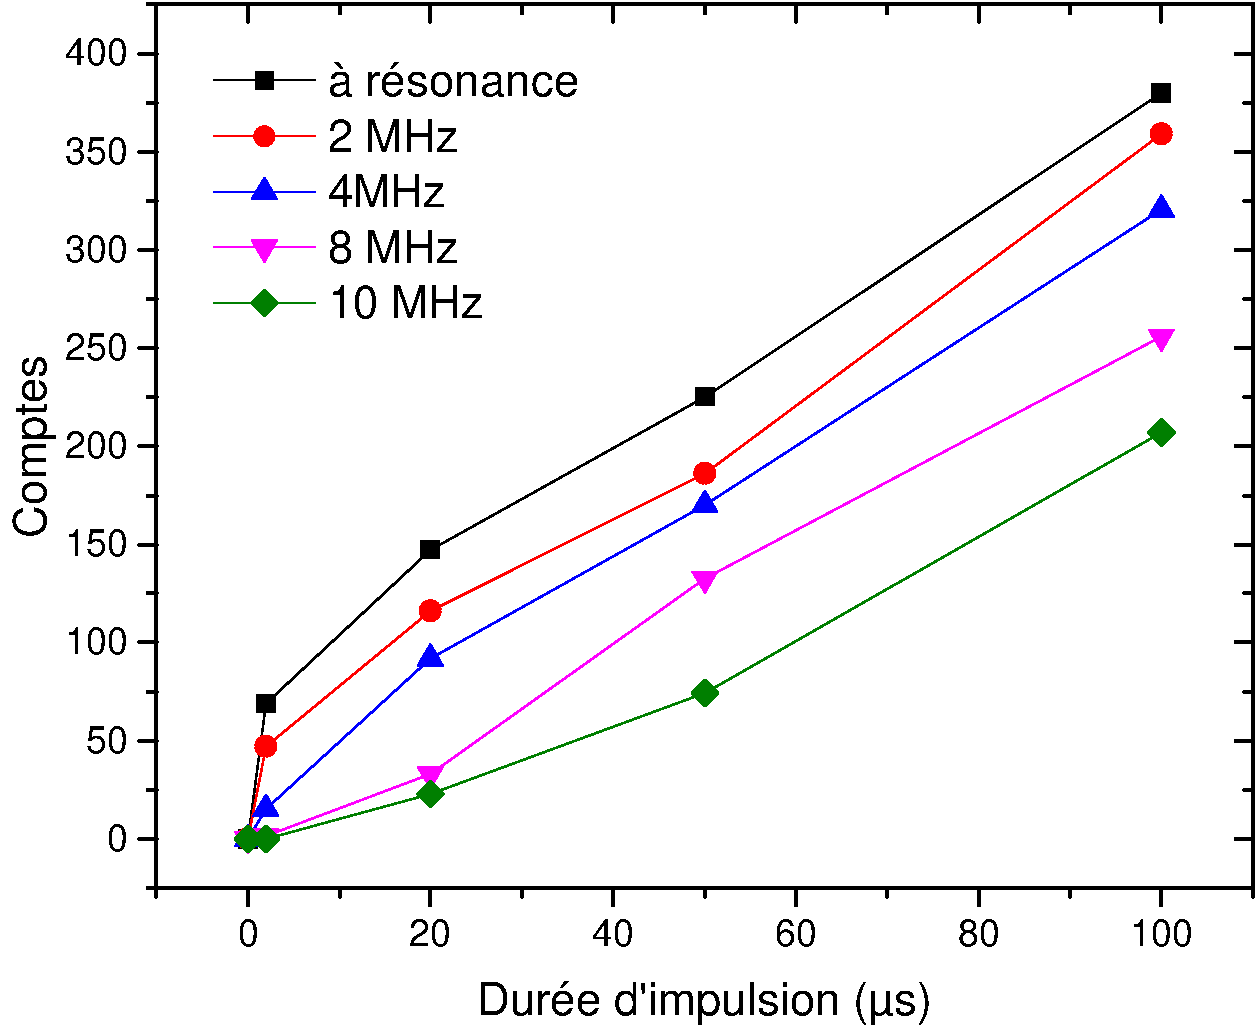
\includegraphics[width=.7\linewidth]{figures/low_l/satur_spectres_optiques_extract}
\caption[Saturation de l'excitation optique en régime d'interaction dipolaire forte]{Saturation de l'excitation optique en régime d'interaction dipolaire forte.
Évolution du nombre d'atomes de Rydberg en fonction de la durée d'impulsion laser, pour différents désaccords : $\SI{0}{}$, $\SI{2}{}$, $\SI{4}{}$, $\SI{8}{}$ et $\SI{10}{MHz}$.
Les données sont extraites des spectres de la figure \eqref{fig:data_spectresoptiques}.
}
\label{fig:data_saturoptique}
\end{figure}
%
On y remarque effectivement qu'à grand désaccord, le nombre d'atomes de Rydberg présente un effet de seuil correspondant à l'excitation non résonante de la \og graine \fg{}.

Le comportement à résonance montre une croissance rapide du nombre d'atomes excités dans les premiers instants, puis une augmentation plus lente.
En effet, le centre du nuage est saturé de super-atomes en régime de blocage fort dès les premières microsecondes.
Ensuite, de nouveaux atomes de Rydberg sont excités dans les ailes peu denses du nuage.
Celles-ci contiennent beaucoup moins d'atomes dans l'état fondamental d'une part, et le laser bleu, dont le col gaussien vaut $\SI{22}{\um}$, y est un peu moins intense d'autre part.
Ces deux facteurs contribuent à ralentir fortement la dynamique d'excitation dans ces régions-là.
Enfin, le mouvement d'expansion du nuage de Rydberg dû aux interactions les éloigne les uns des autres au centre du nuage, où de nouvelles excitations deviennent possibles après quelques dizaines de microsecondes.
Cela peut expliquer pourquoi le nombre d'atomes de Rydberg continue d'augmenter, contrairement aux prédictions de l'approximation du \og gaz gelé \fg{}, qui consiste à considérer que les atomes de Rydberg qui interagissent sont immobiles.% communément utilisée.

	\subsection{Spectroscopie microonde : une sonde pour l'énergie d'interaction} \label{subsec:mw_spectro_exp}
\noindent Afin de mieux comprendre le mouvement au sein du nuage de Rydberg, nous avons réalisé la spectroscopie de la transition $\mathrm{60S} \rightarrow \mathrm{57S}$ dans différentes conditions.
Nous présentons ici le principe de cet outil de spectroscopie microonde comme sonde des énergies d'interaction dans le nuage, et les expériences que nous avons menées.

	\subsubsection*{Principe de la spectroscopie microonde et choix de la transition}
\noindent Comme nous l'avons vu au chapitre \ref{chapter:Rydberg}, les différents niveaux de Rydberg sont affectés différemment par les interactions dipolaires.
En particulier, dans le régime de van der Waals, cela se traduit par des coefficients de van der Waals $C_6$ différents.
Ainsi, le niveau $nS$ et le niveau $n'S$ verront leur énergie déplacée de quantités différentes pour une même distance inter-atomique.
En conséquences, les fréquences de transition entre niveaux de Rydberg seront décalées.
Sonder ces décalages de fréquence, c'est-à-dire faire la spectroscopie de telles transitions, nous renseignera sur la distribution des énergies d'interaction au sein du nuage.
Idéalement, un seul atome du nuage sera transféré vers un autre niveau de Rydberg, et la fréquence de cette transition nous renseignera sur l'énergie d'interaction de cet atome avec tous ses voisins.

Cela requiert cependant un choix attentif du niveau vers lequel seront transférés les atomes de Rydberg.
En premier lieu, les niveaux $P$ sont à éviter.
La branche attractive de l'interaction $n\mathrm{S} - n'\mathrm{P}$ mène à une ionisation de Penning des atomes de Rydberg : l'atome dans le niveau $nS$ et l'atome dans le niveau $n'\mathrm{P}$ s'attirent l'un l'autre, et s'ionisent mutuellement lorsqu'ils sont trop proches.
Nous restreindrons donc notre choix aux niveaux $n'\mathrm{S}$ voisins du $\mathrm{60S}$, accessibles par des transitions à deux photons.

Pour une paire d'atomes séparés de $r$, l'interaction $\mathrm{60S}-n'\mathrm{S}$ prend la forme de l'équation \eqref{eq:MatrixCab_Aab} :
\begin{equation}
\label{eq:Matrix_60SnS}
V_{eff}/h = \bordermatrix{~ 	&\ket{\mathrm{60S,n'S}} 	& \ket{\mathrm{n'S,60S}} \cr
	\bra{\mathrm{60S,n'S}}		&C_{6,\mathrm{60S-n'S}}		&A_{6,\mathrm{60S-n'S}}	\cr 
	\bra{\mathrm{n'S,60S}} 		&A_{6,\mathrm{60S-n'S}}		&C_{6,\mathrm{60S-n'S}} \cr} \ \cdot \frac{1}{r^6},
\end{equation}
%
où $C_6$ et $A_6$ sont les coefficients de van der Waals pour l'interaction directe et pour l'interaction d'échange respectivement.
Les états $\ket{\mathrm{60S,n'S}}$ et $\ket{\mathrm{n'S,60S}}$ sont dégénérés et séparés en leurs combinaisons symétrique et antisymétrique, $(\ket{\mathrm{60S,n'S}}\pm\ket{\mathrm{n'S,60S}})/\sqrt{2}$.
Ces deux états propres sont déplacés d'une énergie $h\cdot (C_{6,\mathrm{60S-n'S}} \pm A_{6,\mathrm{60S-n'S}}) / r^6$.
Cette structure de niveaux est représentée en figure (\ref{fig:60S-nS} a)).
%
\begin{figure}[h]
\centering
\includegraphics[width=\linewidth]{figures/low_l/60S-nS}
\caption[Structure de niveau 60S-nS sous interaction dipolaire]{
Structure de niveau 60S-nS sous interaction dipolaire
\textbf{a)} La paire $\mathrm{60S}-n'\mathrm{S}$ est déplacée en énergie par le terme d'interaction directe $C_{6,\mathrm{60Sn'S}}/r^6$ et ses deux états dégénérés sont séparés par l'interaction d'échange, avec un écart d'énergie de $2A_{6,60Sn'S}/r^6$.
\textbf{b)} Diagramme d'énergie d'une paire dans les niveaux $\mathrm{60S-60S}$ et $\mathrm{60S-57S}$.
Le terme d'échange $A_{6,\mathrm{60S-57S}}$ étant quasi-nul, la dégénérescence des niveaux de paire $\ket{\mathrm{60S,57S}}$ et $\ket{\mathrm{57S,60S}}$ n'est pas levée et la paire se comporte comme un système à deux niveaux.
La transition entre ces deux niveaux est déplacée par les interactions dipolaires.
}
\label{fig:60S-nS}
\end{figure}
%
La levée de dégénérescence des niveaux de paire engendre des spectres à deux raies de transition, séparées en fréquence de $2A_{6,\mathrm{60S-nS}}/r^6$.
Si l'on y ajoute un troisième atome de Rydberg, il y a alors trois paires en interaction, ce qui complexifie d'autant plus la structure de niveaux et le spectre de la transition.
Au sein d'un ensemble de $N$ atomes de Rydberg, les états propres du hamiltonien à une excitation formeront une base très différente de la base séparable $\{\ket{i} = 
\ket{\mathrm{60S}}_1\otimes\dots\otimes\ket{n'S}_i\otimes\dots\otimes\ket{\mathrm{60S}}_N$.
L'excitation de niveau $n'S$ sera ainsi délocalisée sur plusieurs atomes.
On ne peut alors pas directement déduire, du spectre des déplacements d'énergie de cette excitation, la distribution des énergies d'interaction au sein du nuage.

%En fin de compte, au sein d'un ensemble de $N$ atomes de Rydberg dans le niveau $\mathrm{60S}$, une  excitation du niveau $n'S$ sera délocalisée sur des états propres à $N$ atomes.
%Ces états propres sont des combinaisons linéaires de la base séparable $\{\ket{i} = 
%\ket{\mathrm{60S}}_1\otimes\dots\otimes\ket{n'S}_i\otimes\dots\otimes\ket{\mathrm{60S}}_N$,
%%\ket{1=\mathrm{60S},\dots,i=n'S,\dots,N=\mathrm{60S}} \}_{i=1\text{ à } N}$
%très dépendantes de la configuration du nuage.
%Plus la base des états propres à une excitation est différente de la base des $\ket{i}$, plus le spectre d'excitation devient difficile à relier aux énergies d'interaction.

Le niveau $n'\mathrm{S}$ idéal serait donc celui pour lequel les états propres à une excitation sont ceux où l'excitation est localisée sur un atome.
Pour cela, le terme d'échange $A_6$, responsable de la délocalisation de l'excitation, doit être le plus petit possible, c'est-à-dire très petit devant $C_6$.
La table \eqref{tab:VdW-60SnS} répertorie les coefficients de van der Waals $C_{6,\mathrm{60S-n'S}}$ et $A_{6,\mathrm{60S-n'S}}$ pour les niveaux $n'\mathrm{S}$ proches du $\mathrm{60S}$.
%
\begin{table}[!h]
	\centering
	\caption[Coefficients de van der Waals pour différents niveaux $60S-n'\mathrm{S}$]{Coefficients de van der Waals pour différents niveaux $60S-n'\mathrm{S}$
	}
	\label{tab:VdW-60SnS}
	\begin{tabular}{c c c}
		\toprule\midrule
		~
		& $C_{6,\mathrm{60S-n'S}}$
		& $A_{6,\mathrm{60S-n'S}}$\\		
		~
		& $(\si{\GHz\raiseto{6}\um})$
		& $(\si{\GHz\raiseto{6}\um})$\\
		\midrule
		60S-63S & \SI{-89.26}{} & \SI{0.61}{} \\
		60S-62S & \SI{-411.36}{} & \SI{14.96}{} \\
		60S-61S & \SI{292.25}{} & \SI{248.60}{} \\
		60S-60S & \SI{137.62}{} & \SI{}{} \\
		60S-59S & \SI{245.13}{} & \SI{209.55}{} \\
		60S-58S & \SI{-209.26}{} & \SI{7.77}{} \\
		60S-57S & \SI{-43.67}{} & \SI{0.30}{} \\
		\midrule
		\bottomrule
 	\end{tabular}
\end{table}
%
On y trouve les niveaux $\mathrm{63S}$ et $\mathrm{57S}$, qui présentent des termes d'échanges avec le $\mathrm{60S}$ petits devant les termes d'interaction directe ($C_6 / A_6 \sim 150$).
Étant donné le caractère attractif de l'interaction directe pour les paires $\mathrm{60S-57S}$ et $\mathrm{60S-63S}$, il est préférable de choisir la plus petite de ces interactions afin de limiter le processus d'ionisation de Penning que nous décrivions pour les paires $nS-n'P$.

Nous choisirons donc, pour faire la spectroscopie microonde du nuage de Rydberg, la transition $\mathrm{60S-57S}$.
Nous disposerons ainsi d'un diagramme d'énergie simple, représenté pour deux atomes en figure (\ref{fig:60S-nS} b)), fournissant un système effectif à deux niveaux.
Lorsque les deux atomes n'interagissent pas, la transition à deux photons du niveau de paire $\ket{\mathrm{60S,60S}}$ vers les niveaux de paire dégénérés $\ket{\mathrm{57S,60S}}$ et $\ket{\mathrm{60S,57S}}$ se fait à une fréquence $\nu_0 = 2\times \SI{58.229}{\GHz}$.
En présence d'interactions, la transition est déplacée d'une quantité
\begin{equation}
\label{eq:60s-57s_2atoms}
\Delta\nu (r) = \frac{C_{6,\mathrm{60S-60S}}-C_{6,\mathrm{60S-57S}}}{r^6} = \eta \frac{C_{6,\mathrm{60S-60S}}}{r^6},
\end{equation}
avec $\eta = 1-C_{6,\mathrm{60S-57S}}/C_{6,\mathrm{60S-60S}} = \num{1.317}$.

La généralisation à un ensemble de $N$ atomes de Rydberg se fait dans l'hypothèse d'additivité des interactions de van der Waals.
Ils sont initialement tous dans l'état $\mathrm{60S}$, et l'on suppose que l'impulsion microonde de spectroscopie ne crée qu'une seule excitation $\mathrm{57S}$.
Grâce à la faiblesse du terme d'échange $A_{6,60S57S}$, nous pouvons supposer que cette excitation sera localisée sur un atome de l'ensemble, l'atome $i$, cependant que tous les autres resteront dans l'état $\mathrm{60S}$.
L'énergie d'interaction de l'atome $i$ avant excitation est, comme à l'équation \eqref{eq:Eint_isum}, de
\begin{equation}
\label{eq:Eint_i60S}
E_{int}(i,60S) = hC_{6,60S60S}\sum_{j\neq i} \frac{1}{r_{ij}^6}.
\end{equation}
Lorsque l'atome $i$ est transféré dans l'état $\mathrm{57S}$, son énergie d'interaction devient
\begin{equation}
\label{eq:Eint_i57S}
E_{int}(i,57S) = hC_{6,60S57S}\sum_{j\neq i} \frac{1}{r_{ij}^6}.
\end{equation}
Le déplacement en fréquence de la transition $\mathrm{60S-57S}$ de l'atome $i$, dû aux interactions dipolaires, vaut donc, sous l'hypothèse \og d'atome unique \fg{} que l'atome $i$ est le seul transféré vers le niveau $\mathrm{57S}$,
\begin{equation}
\label{eq:DeltaNu_i}
\Delta\nu (i) = \frac{1}{h}(E_{int}(i,60S)-E_{int}(i,57S)) = \eta \frac{E_{int}(i,60S)}{h}.
\end{equation}

Ce système à $N$ atomes est représenté en figure \eqref{fig:60S-57S_Nat}.
%
\begin{figure}[t]
\centering
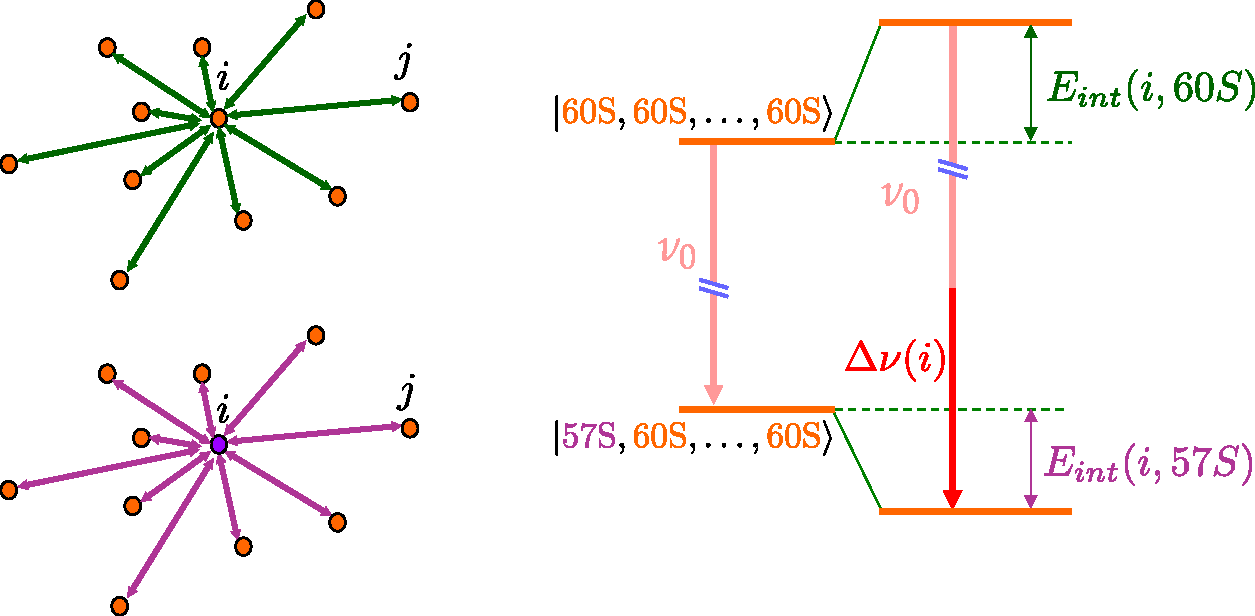
\includegraphics[width=\linewidth]{figures/low_l/60S-57S_Nat}
\caption[Structure de niveaux d'un nuage de $\mathrm{60S}$ contenant une excitation $\mathrm{57S}$]{
Structure de niveaux d'un nuage de $\mathrm{60S}$ contenant une excitation $\mathrm{57S}$.
La faiblesse du terme d'échange dans l'interaction $\mathrm{60S-57S}$ permet que cette excitation soit localisée sur un atome $i$.
La transition microonde permettant de transférer l'atome $i$ est décalée en fréquence d'une quantité $\Delta\nu(i)$ par les interactions dipolaires.
}
\label{fig:60S-57S_Nat}
\end{figure}
%
On peut ainsi sonder la distribution des énergies d'interaction au sein du nuage.
En effet, la probabilité qu'un atome $i$ voie sa fréquence de transition déplacée de $\Delta\nu (i) = \Delta \nu$ est égale à la probabilité que son énergie d'interaction ait été de $E_{int}(i,60S) = h\Delta\nu/\eta$ :
\begin{equation}
P\left( \frac{}{} \!\Delta\nu(i)=\Delta\nu \right )
=P \left( \eta\frac{E_{int}(i,60S)}{h} = \Delta\nu \right) = P\left( E_{int}(i,60S) = \frac{h\Delta\nu}{\eta}% = E_{int}
\right).
\end{equation}
%Le spectre de la transition microonde, qui mesure la distribution de probabilité $P(\Delta\nu)$ au sein d'un nuage, mesure à un facteur $\eta$ près la distribution de probabilité $P(E_{int}$ des énergies d'interactions dans le nuage.
Du spectre microonde de la transition, qui représente la distribution $P(\Delta\nu)$, on déduit directement la distribution $P(E_{int})$ des énergies d'interaction dans le nuage par la transformation $\Delta\nu = \eta E_{int}/h$.

	\subsubsection*{Spectres des énergies d'interaction}
\noindent Cet outil de spectroscopie microonde nous a servi à sonder les énergies d'interaction au sein de différents nuages de Rydberg.
\`A partir d'une excitation laser d'une durée de $\SI{2}{\us}$, telle que décrite en \ref{subsec:optical_spectra}, nous sélectionnons différents désaccords laser.
%Nous sonderons ainsi un nuage excité à résonance $(\Delta = 0)$ en régime de blocage dipolaire fort, un nuage excité avec un désaccord $\Delta = \SI{1}{MHz}$ et un nuage excité avec un désaccord $\Delta = \SI{2}{\MHz}$.
Une impulsion microonde sur la transition $\mathrm{57S-60S}$ est envoyée immédiatement après l'impulsion laser d'excitation.
La fréquence de cette impulsion est balayée de façon à obtenir la distribution $P(h\Delta\nu/\eta)$ des énergies d'interaction.
Nous en obtiendrons la distribution des énergies d'interaction dans trois cas  : sous blocage dipolaire fort ($\Delta = 0$), sous excitation facilitée ($\Delta = \SI{2}{\MHz}$), et dans un régime intermédiaire ($\Delta = \SI{1}{\MHz}$).
La séquence expérimentale et les spectres obtenus sont représentés en figure \eqref{fig:microwave_probe_0delay}.

\begin{figure}[h]
\centering
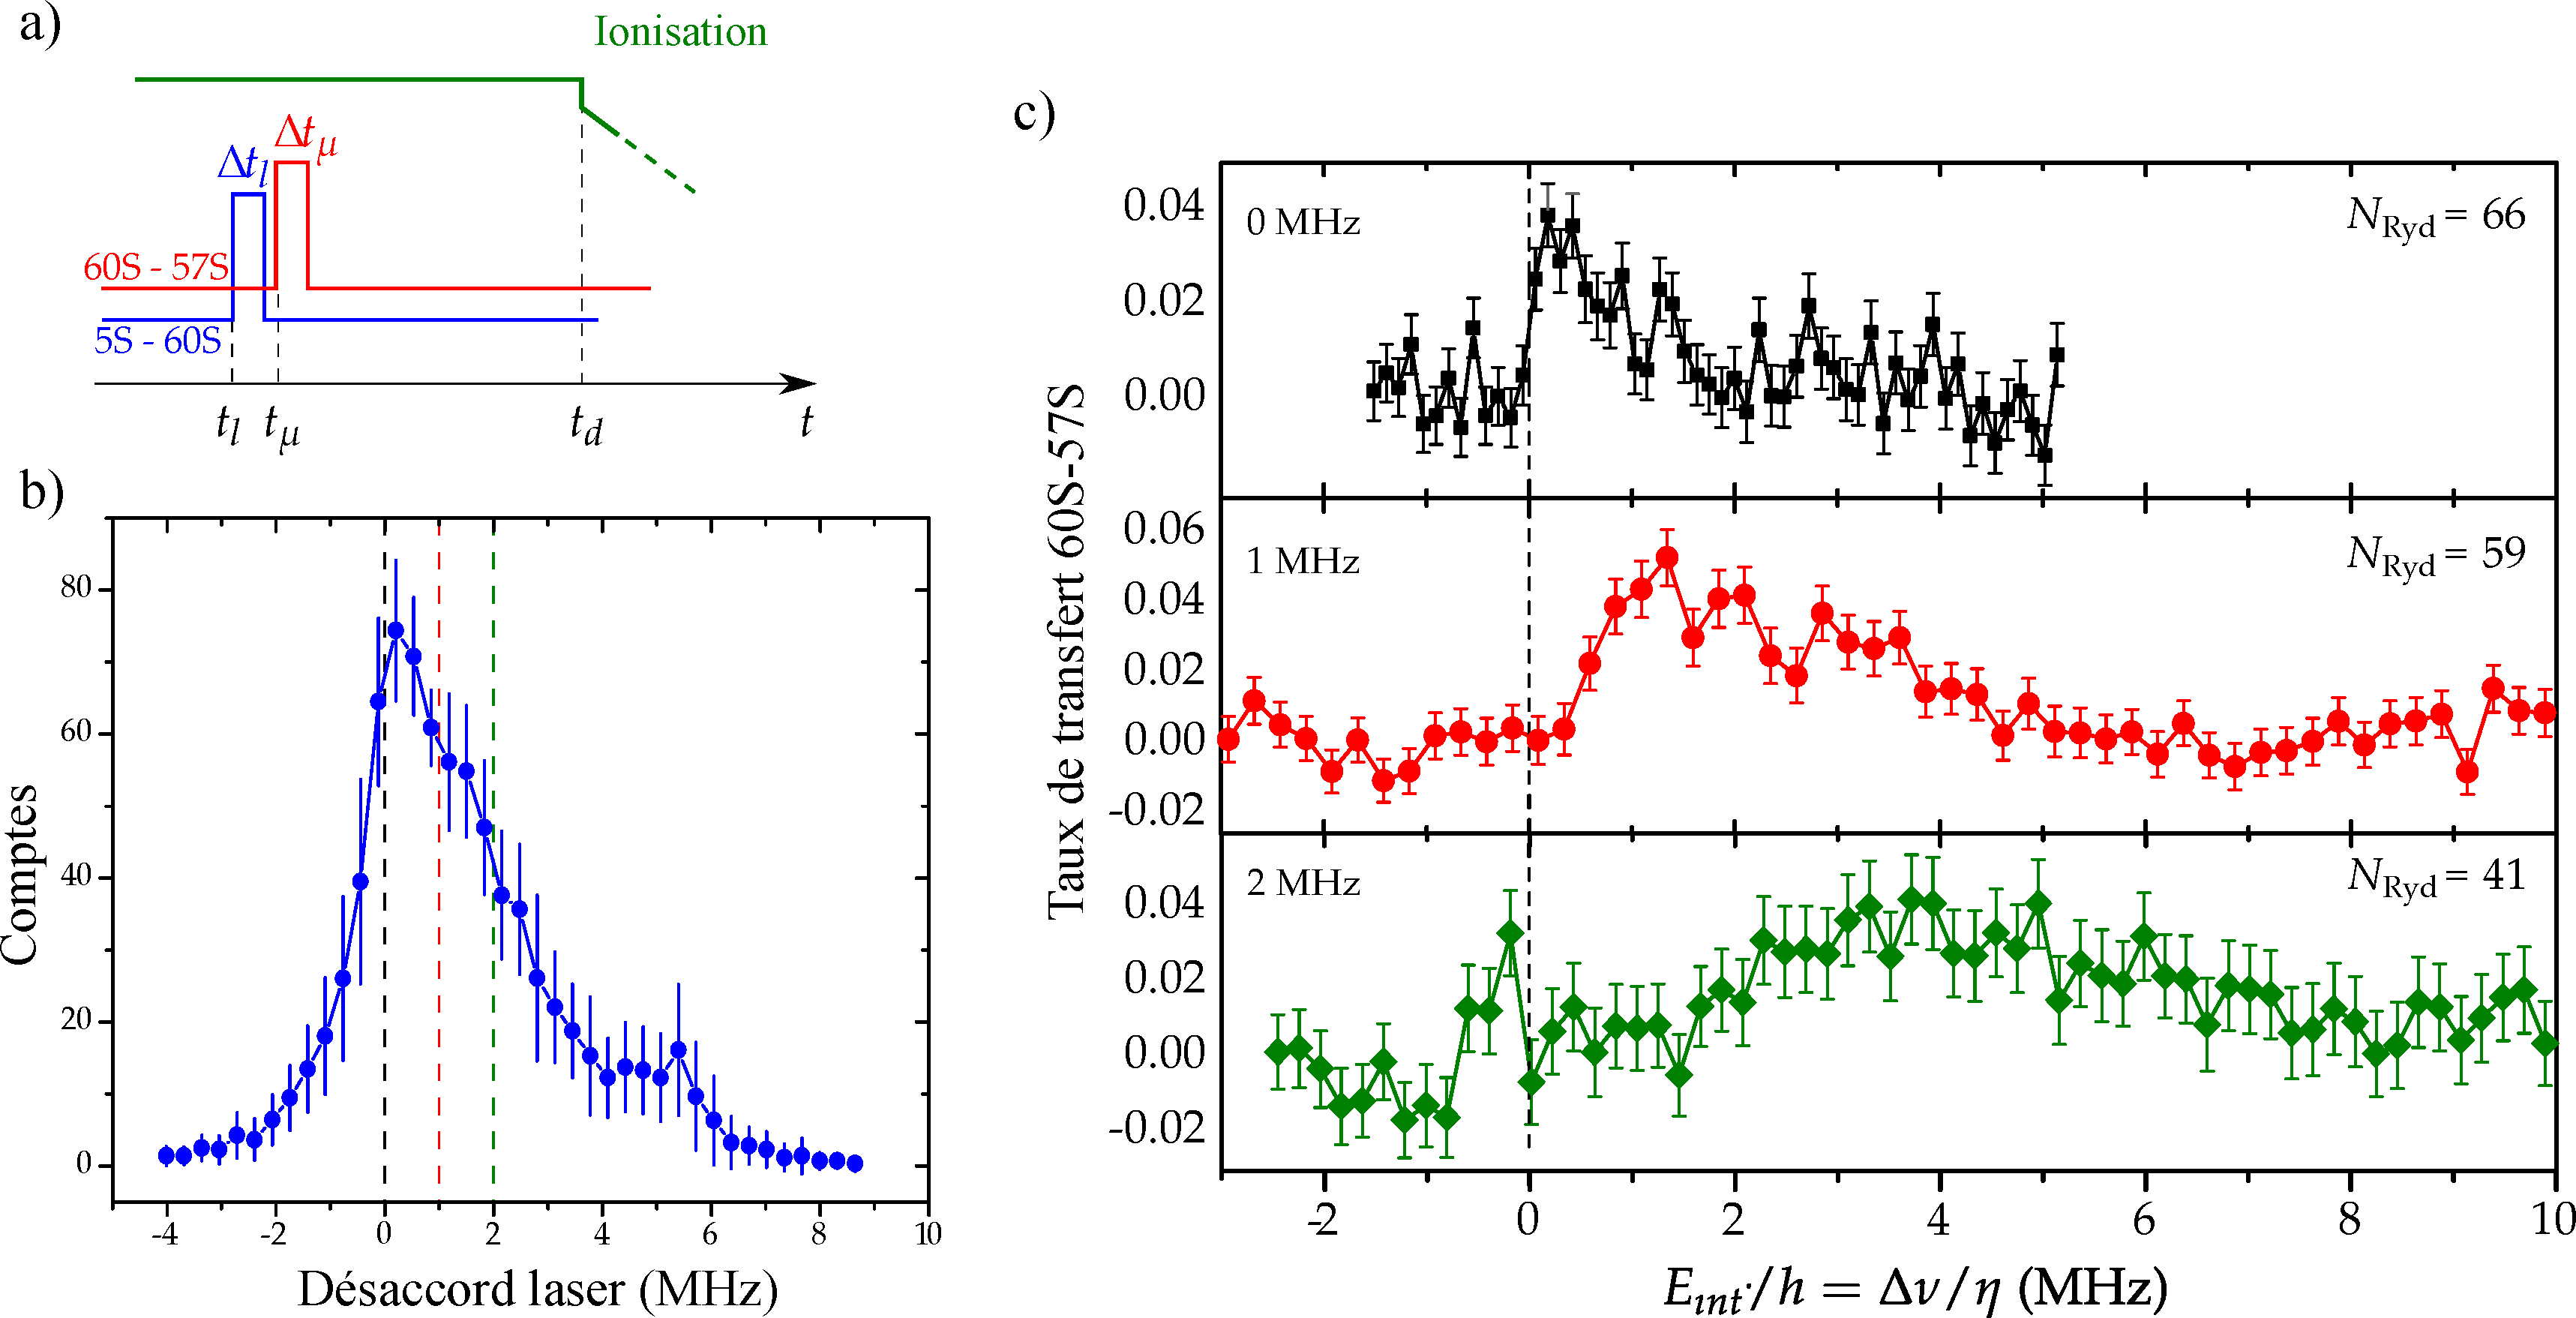
\includegraphics[width=\linewidth]{figures/low_l/microwave_probe_0delay_wide}
\caption[Spectroscopie microonde du nuage avec expansion]{
Spectroscopie microonde du nuage avant expansion.
\textbf{a)} Séquence expérimentale de la spectroscopie : une impulsion laser envoyée à l'instant $t_l$ et d'une durée de $\Delta t_l$ est suivie d'une impulsion microonde, envoyée à l'instant $t_\mu$ et durant $\Delta t_\mu$.
La détection est effectuée par une rampe d'ionisation déclenchée à l'instant $t_d$.
\textbf{b)} Spectre laser de la transition $\mathrm{5S-60S}$. Les lignes pointillées marquent les désaccord choisis de $\SI{0}{}$, $\SI{1}{}$ et $\SI{2}{\MHz}$.
\textbf{c)} Spectres microonde de la transition $\mathrm{60S-57S}$ pour différents désaccords laser $\Delta = 0, 1 , \SI{2}{\MHz}$.
}
\label{fig:microwave_probe_0delay}
\end{figure}

La fraction atomique transférée vers le niveau $\mathrm{57S}$ est tracée comme fonction de l'énergie d'interaction, c'est-à-dire du déplacement en fréquence de la transition renormalisé $\Delta\nu/\eta$.
Le faible nombre d'excitations vers le $\mathrm{57S}$ permet de confirmer l'hypothèse d'atome unique qui justifie la méthode de spectroscopie par l'équation \eqref{eq:DeltaNu_i} : nous ne transférons jamais plus de $\SI{3}{}$ atomes vers le niveau $\mathrm{57S}$ et ils sont suffisamment éloignés les uns des autres pour n'interagir qu'avec des atomes dans le niveau $\mathrm{60S}$.
On peut redouter une ionisation de Penning entre les atomes dans le niveau $\mathrm{57S}$ et les atomes dans le niveau $\mathrm{60S}$ en raison de l'attractivité de leur interaction.
Cependant, cette interaction est suffisamment faible pour que les atomes soient détectés avant que cela ne se produise. %\footnote{
%Nous pouvons confirmer cela à l'étude des signaux d'ionisation, qui montrent l'absence d'ions préexistant à la rampe de détection.}.

En figure (\ref{fig:microwave_probe_0delay} c)), l'axe des abscisses donne directement l'énergie d'interaction $E_{int}$ des atomes.
Or, d'après l'équation \eqref{eq:Eint_i60S}, le plus proche voisin d'un atome ayant une énergie d'interaction $E_{int}$ ne peut être à une distance de celui-ci inférieure à $r_E(E_{int}) = (hC_{6,\mathrm{60S-60S}}/E_{int})^{1/6}$.
\`A désaccord laser nul $\Delta = 0$, le spectre microonde est déplacé d'environ la largeur laser $\gamma/2$, ce qui tend à confirmer le fait que le nuage est saturé de super-atomes.
En effet dans ce cas, chaque atome de Rydberg a au moins un voisin à une distance d'un rayon de blocage $r_b$ et donc avec une interaction d'énergie $E_{int}(r_b) = \gamma/2$.
Chaque voisin supplémentaire augmente l'énergie d'interaction d'au maximum $\gamma/2$, expliquant la queue du spectre jusqu'à $\SI{2}{\MHz}$ pour les atomes ayant le plus de voisins.
Enfin, l'absence de signal au-delà de $E_{int} = \SI{2}{\MHz}$ indique l'absence de paires atomique séparées de moins de $r_E(\SI{2}{\MHz}) = \SI{6.4}{\um}$, en raison du blocage dipolaire.
	
Aux désaccords laser positifs $\Delta > 0$, le mécanisme de facilitation excite le nuage de Rydberg avec, pour chaque nouvel atome, une énergie d'interaction égale à $\Delta$.
Cela décale le spectre vers les hautes énergies, en excitant des atomes de Rydberg de plus en plus proches les uns des autres à mesure qu'augmente le désaccord $\Delta$.
Le désaccord positif du laser produit ainsi un agrégat de Rydberg.
Au c\oe ur de cet agrégat, chaque atome de Rydberg a plusieurs voisins, qui contribuent tous à augmenter son énergie d'interaction.
De même que dans le cas $\Delta = 0$ du blocage dipolaire fort, les queues à haute fréquence  des spectres sont attribuées à ces atomes du centre du nuage.
La figure \eqref{fig:clustering} représente la formation d'un tel agrégat de Rydberg et l'accumulation de l'énergie d'interaction qui s'en suit.

\begin{figure}[h]
\centering
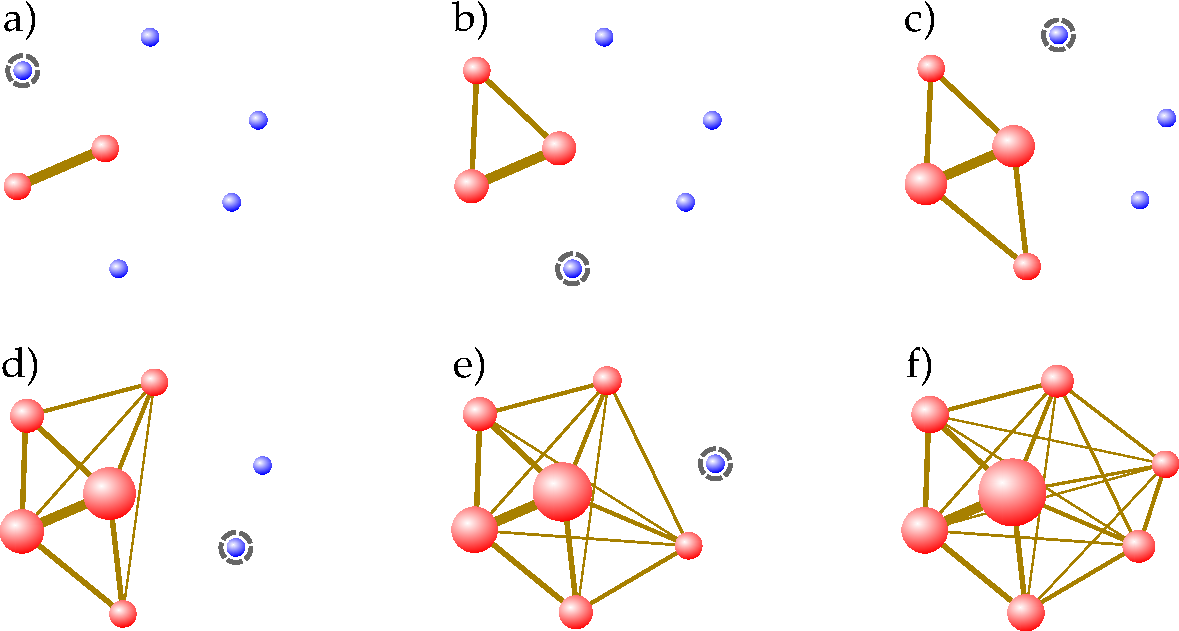
\includegraphics[width=.7\linewidth]{figures/low_l/accumulation_2D}
\caption[Formation d'un agrégat de Rydberg et accumulation de l'énergie d'interaction]{
Formation d'un agrégat de Rydberg et accumulation de l'énergie d'interaction, de \textbf{a)} à \textbf{e)}.
Les sphères bleues représentent des atomes dans l'état fondamental et les sphères rouges des atomes de Rydberg.
Les cercles pointillés autour des sphères bleues signalent quel atome sera excité à l'étape suivante.
L'épaisseur de la ligne joignant deux atomes de Rydberg représente la force de l'interaction entre ces deux atomes.
La taille de chaque sphère rouge représente l'énergie d'interaction totale de l'atome de Rydberg correspondant.
}
\label{fig:clustering}
\end{figure}
%

\newpage
\subsubsection*{Évolution au cours du temps : explosion du nuage}
\noindent Après excitation, le nuage de Rydberg explose sous l'effet des interactions dipolaires répulsives entre atomes de Rydberg dans le niveau $\mathrm{60S}$.
La spectroscopie microonde nous permet, de la même façon que précédemment, de mesurer les énergies d'interaction dans le nuage au cours de cette explosion.
Il suffit pour cela d'introduire un délai variable $\Delta t$ entre l'excitation laser et l'impulsion microonde de sonde.

Les spectres ainsi obtenus sont représentés en figure \eqref{fig:microwave_explosion}, pour des désaccords laser de $\Delta = 0, 1$ et $\SI{2}{\MHz}$.
\`A mesure que le temps avance, les distributions d'énergie d'interaction s'affinent et tendent vers celle d'un nuage dilué sans interaction.
Cette énergie d'interaction est convertie en énergie cinétique au cours de l'explosion du nuage de Rydberg.
La figure \eqref{fig:avener_explosion} représente l'énergie moyenne d'un nuage au cours du temps, pour les trois mêmes désaccords laser.

L'énergie moyenne initiale est de l'ordre de $\SIrange{1}{10}{\MHz}$ dans les trois cas.
En comparaison, l'énergie cinétique des atomes dans le niveau fondamental, refroidis à $\SI{500}{\nano\K}$ est de l'ordre de $\SI{10}{\kHz}$, donc négligeable.
L'évolution des spectres microonde peut être entièrement attribuée à l'explosion du nuage de Rydberg en interaction.

Le mouvement des atomes de Rydberg devient important dès lors qu'il modifie sensiblement la distribution des énergies d'interaction, donc les spectres microonde mesurés.
Ainsi nous pouvons affirmer qu'après un délai aussi court que $\Delta t \sim \num{5}$ à $\SI{10}{\us}$, le mouvement a modifié la configuration énergétique du nuage, y compris lorsque celui-ci a été excité à résonance.
L'approximation du \og gaz gelé \fg{} ne peut donc être considérée comme valide au delà de quelques microsecondes dans un nuage dense d'atomes de Rydberg.

\clearpage

\begin{figure}[t]
\centering
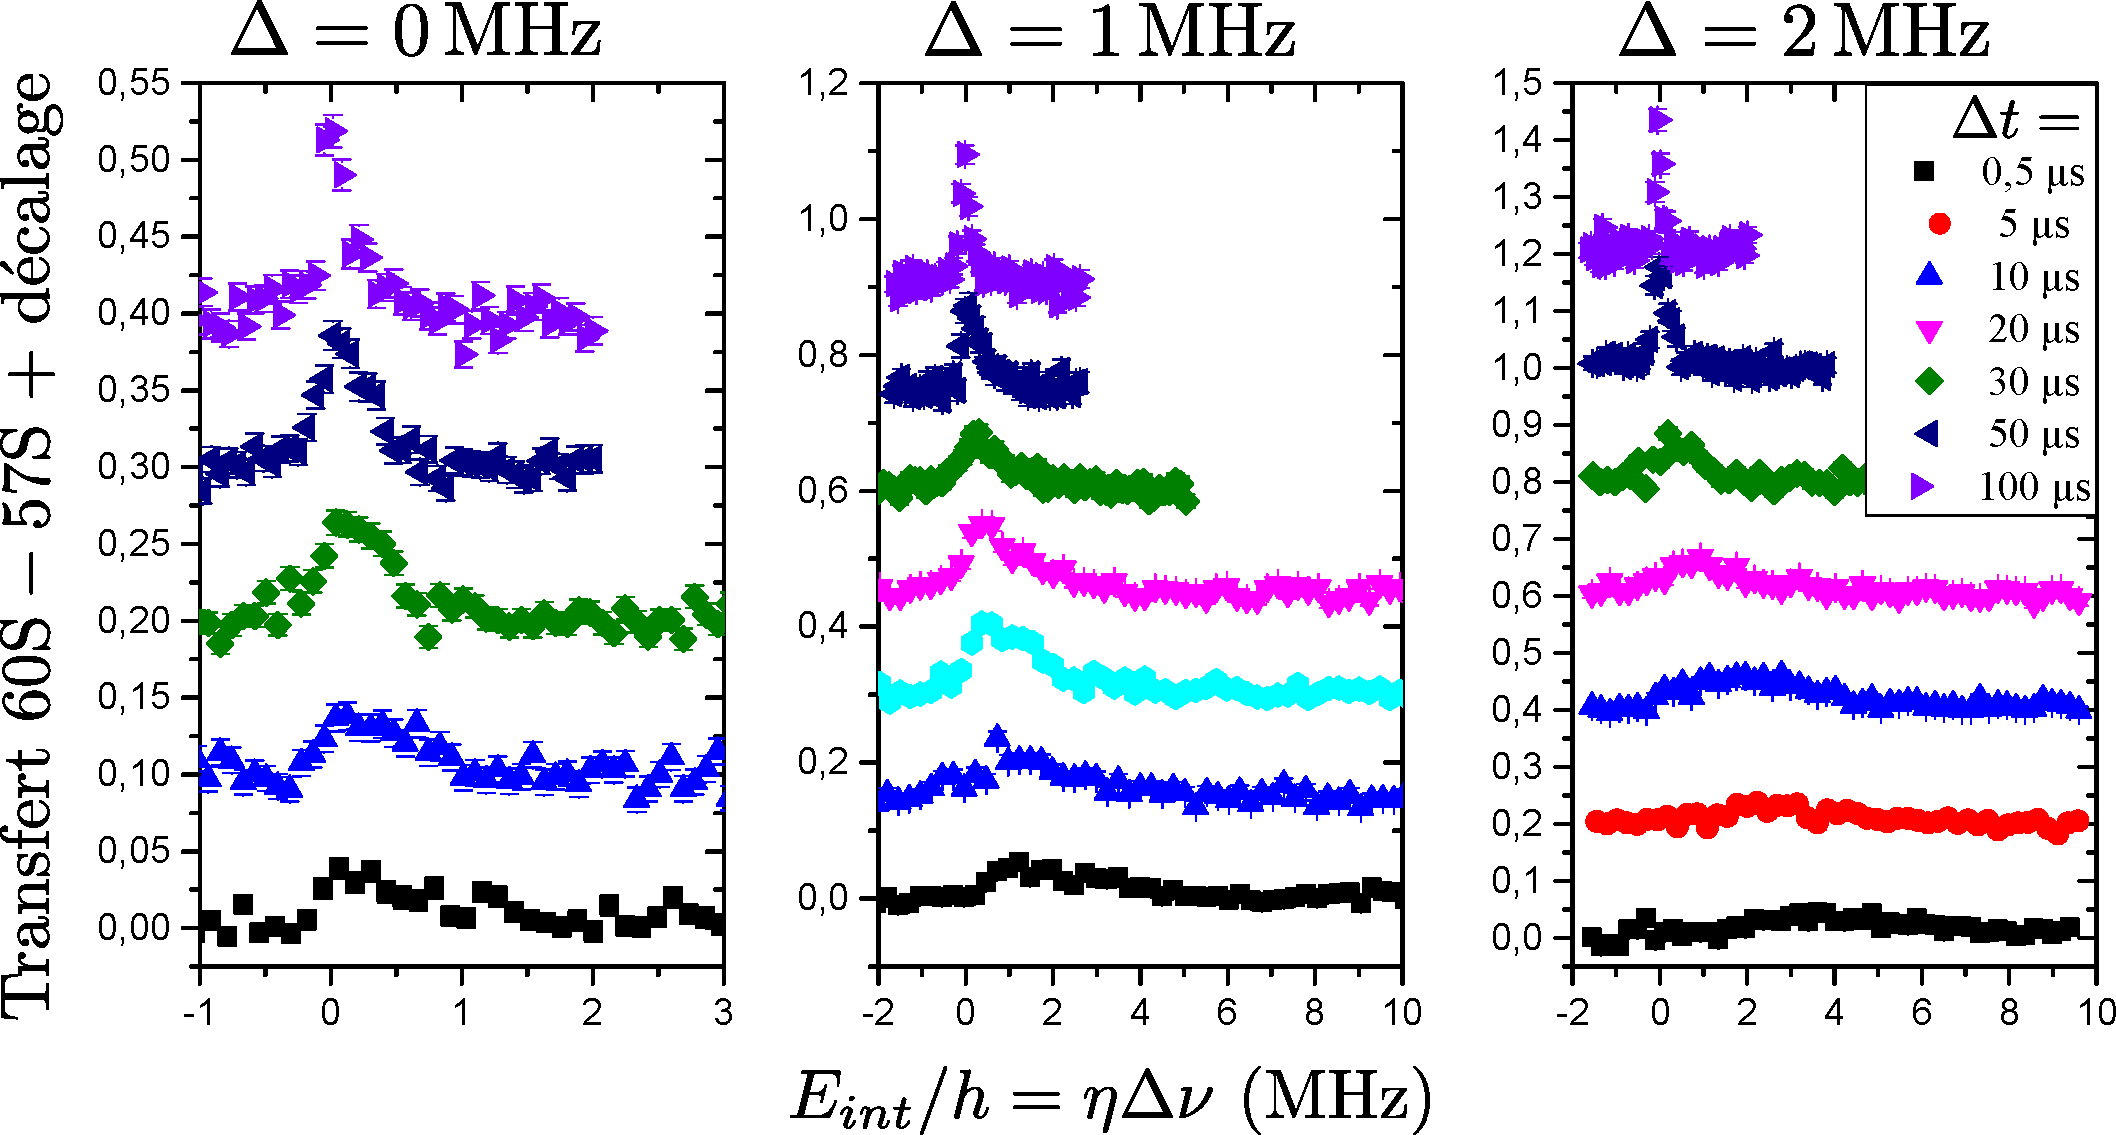
\includegraphics[width=\linewidth]{figures/low_l/expansion_012MHz}
\caption[Spectroscopie microonde de l'expansion du nuage]{
Spectres microonde de la transition $\mathrm{60S-57S}$ au cours de l'évolution d'un nuage de Rydberg excité par un laser désaccordé à $\Delta= 0$ (gauche), $\SI{1}{\MHz}$ (centre) et $\SI{2}{\MHz}$ (droite).
L'origine des axes verticaux de chacun des spectres est décalée et l'échelle des abscisses et des ordonnées de chacun des graphes est différente, par souci de visibilité.
}
\label{fig:microwave_explosion}
\end{figure}

\begin{figure}[b]
\centering
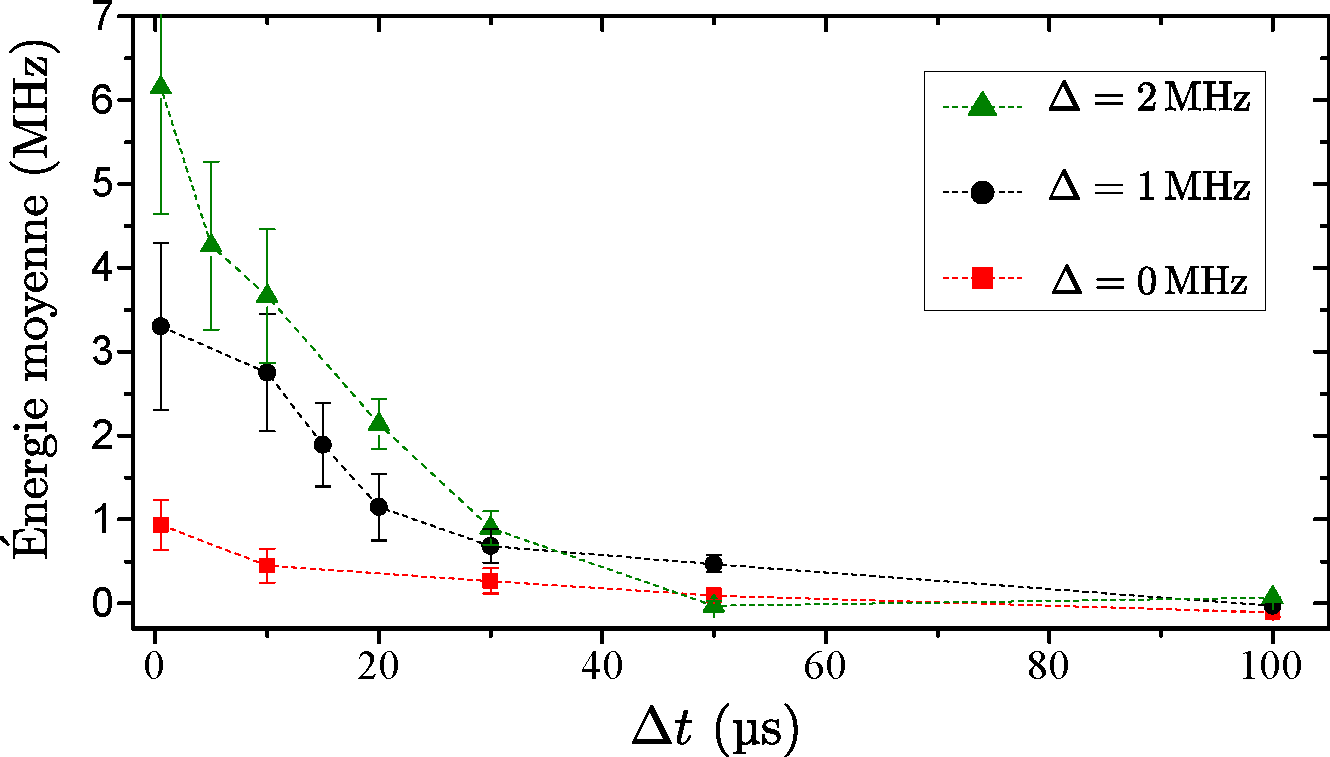
\includegraphics[width=0.8\linewidth]{figures/low_l/energie_moyenne_explosion}
\caption[Énergie moyenne au cours de l'expansion du nuage]{
Énergie moyenne d'interaction (énergie totale rapportée au nombre d'atomes) de nuages de Rydberg excités à différents désaccords laser, en fonction du temps après excitation $\Delta t$.
Les données sont calculées à partir des spectres de la figure \eqref{fig:microwave_explosion}.
}
\label{fig:avener_explosion}
\end{figure}

\clearpage
\section{Premier modèle numérique et accord qualitatif}
\noindent Afin d'affiner notre compréhension de ces phénomènes dûs aux interactions, nous avons développé un modèle numérique de nos expériences.
L'intégration numérique de l'équation de Schrödinger dépendante du temps pour un nuage de $\SI{12000}{}$ atomes corrélés étant irréaliste, nous avons établi un modèle Monte Carlo.

Le calcul numérique est effectué en deux phases distinctes : la première simule la dynamique d'excitation du nuage de Rydberg à partir des atomes dans l'état fondamental.
Une fois l'excitation terminée, l'explosion du nuage de Rydberg est calculée comme un problème classique à $N$ corps, par une routine d'intégration de Runge-Kutta d'ordre $4$.

Nous donnons ici une description fonctionnelle de l'algorithme et comparons ses résultats aux résultats expérimentaux.

	\subsection{Au c\oe ur du modèle numérique}\label{subsec:algo_1}
\noindent Le premier modèle de l'excitation que nous avons mis en \oe uvre est présenté en détail dans le chapitre IV de la thèse de Raul Celistrino Teixeira \cite{PHD_CELISTRINO}.
Il fonctionne de la manière suivante :
\begin{enumerate}
	\item Un nuage de $N$ atomes dans l'état fondamental est tiré au sort selon une distribution gaussienne, dont les paramètres sont l'extension spatiale du piège selon chaque direction, $\sigma_x,\sigma_y,\sigma_z$.
	\item Le profil gaussien de l'intensité laser est spécifié, paramétrés par les cols des faisceaux bleus et rouges.
	\item Le profil de la raie d'excitation à un atome est donné, correspondant au spectre \og référence piège dilué \fg{} de la figure \eqref{fig:data_spectresoptiques}.
	\item \`A chaque itération, un atome $i$ de l'état fondamental est tiré au sort.
	Son énergie d'interaction totale $E_{int}(i)$ avec les atomes de Rydberg déjà présents est calculée comme s'il était excité.
	La probabilité d'excitation $p(i)$ de l'atome est calculée d'après le profil de raie laser, en fonction de l'intensité  et du désaccord $\Delta$ du laser et de l'énergie d'interaction $E_{int}(i)$.
	\item La probabilité $p(i)$ est comparée à un nombre aléatoire $x$ entre $0$ et $1$. Si $x > p(i)$, la simulation passe à l'itération suivante.
	Si $x\leq p(i)$, alors l'atome $i$ est excité au niveau de Rydberg et ajouté à la liste de ceux-ci.
\end{enumerate}
%
Dans ce modèle, l'excitation d'un atome se fait sous la forme d'un \og saut \fg{} de l'état fondamental à l'état de Rydberg.
Cela exclut de fait tout processus cohérent au cours duquel une superposition d'état serait créée.
L'algorithme ici présenté ne peut d'ailleurs rendre compte que d'une excitation séquentielle des atomes de Rydberg les uns après les autres.
De plus, le nuage d'atomes de Rydberg est considéré comme gelé lors de l'excitation.
Bien que cette hypothèse puisse être raisonnable pour une durée d'impulsion laser de $\SI{2}{\us}$, les résultats expérimentaux nous apprennent qu'elle ne le sera plus pour des durées d'excitation supérieures à $\SI{10}{\us}$.

Enfin, notons que ce modèle ne comporte aucune échelle de temps durant l'excitation.
Un critère sera donc nécessaire pour déterminer la fin du calcul.
Pour simuler les spectres d'énergie d'interaction et leur évolution dans le temps, le désaccord laser $\Delta$ et la durée d'impulsion sont fixés.
Les spectres laser expérimentaux nous renseignent alors sur le nombre $N_{Ryd}$ d'atomes de Rydberg que contient le nuage au terme de l'excitation.
C'est ce nombre $\Nryd$ qui sert de critère à l'arrêt du calcul : une fois celui-ci atteint, l'excitation est terminée et le calcul de l'explosion du nuage commence.

Le calcul de l'expansion du nuage se déroule de la manière suivante :
\begin{enumerate}
\item \label{item:init_explosion}Les données de départ sont les positions et quantités de mouvement des atomes de Rydberg excités à l'étape précédente de la simulation.
\`A partir de ces positions, les énergies d'interaction sont calculées pour chaque paire d'atomes de Rydberg.
\item Ces énergies d'interaction sont dérivées d'après l'équation \eqref{eq:repuls_2atoms}, puis sommées pour chaque atome d'après l'équation \eqref{eq:repuls_Natomes}.
La force mécanique appliquée à chaque atome de Rydberg par le reste du nuage est ainsi obtenue.
\item Un routine Runge-Kutta d'ordre $4$ permet de calculer les positions et quantités de mouvement des atomes de Rydberg après un pas de temps $dt$.
\item L'algorithme retourne à l'étape \ref{item:init_explosion} et réitère le calcul avec les positions et quantités de mouvement actualisées.
\end{enumerate}
Lorsque le temps total d'évolution est atteint, les énergies d'interaction totales de chaque atomes sont calculées et compilées sous forme d'un spectre que l'on pourra comparer aux spectres microonde de la figure \eqref{fig:microwave_explosion}.
Le temps de vie des atomes de Rydberg est pris en compte au cours de ce calcul, en permettant la désexcitation de chaque atome avec un taux de probabilité $e^{-t/\tau}$, où $t$ est le temps écoulé depuis l'excitation et $\tau = \SI{210}{\us}$ est le temps de vie du niveau $\mathrm{60S}$ mesuré expérimentalement (cf \ref{subsec:lifetime}).
Enfin, les spectres expérimentaux sont réalisés avec des impulsions microonde de durée comprise entre $\SI{1}{}$ et $\SI{6}{\us}$.
%limités par transformée de Fourier en raison de la durée finie de l'impulsion microonde de sonde.
Les spectres microonde simulés seront donc finalement convolués avec la transformée de Fourier de l'impulsion microonde, et pourront être confrontés aux spectres expérimentaux.

\subsection{Comparaison aux spectres microonde expérimentaux}
\noindent Étant donnée que le modèle présenté ci-dessus ne tient pas compte du mouvement des atomes de Rydberg durant l'excitation, sa validité est \textit{a priori} restreinte aux durées d'impulsion laser courtes.
De même, choisir comme critère d'arrêt le nombre d'atomes de Rydberg final empêche d'utiliser ce modèle pour simuler les spectres d'excitation optique présentés en \ref{subsec:optical_spectra}.
Nous nous limiterons pour le moment à comparer les simulations aux spectres microonde présentés en \ref{subsec:mw_spectro_exp}.

La première étape de cette comparaison consiste à vérifier l'accord entre les spectres simulés et les distributions d'énergie d'interaction immédiatement après excitation, qui sont présentées en figure \eqref{fig:microwave_probe_0delay}.
La figure \eqref{fig:micro_0delay_firstTest} présente ces mêmes spectres comparés aux simulations.
%
\begin{figure}[h]
\centering
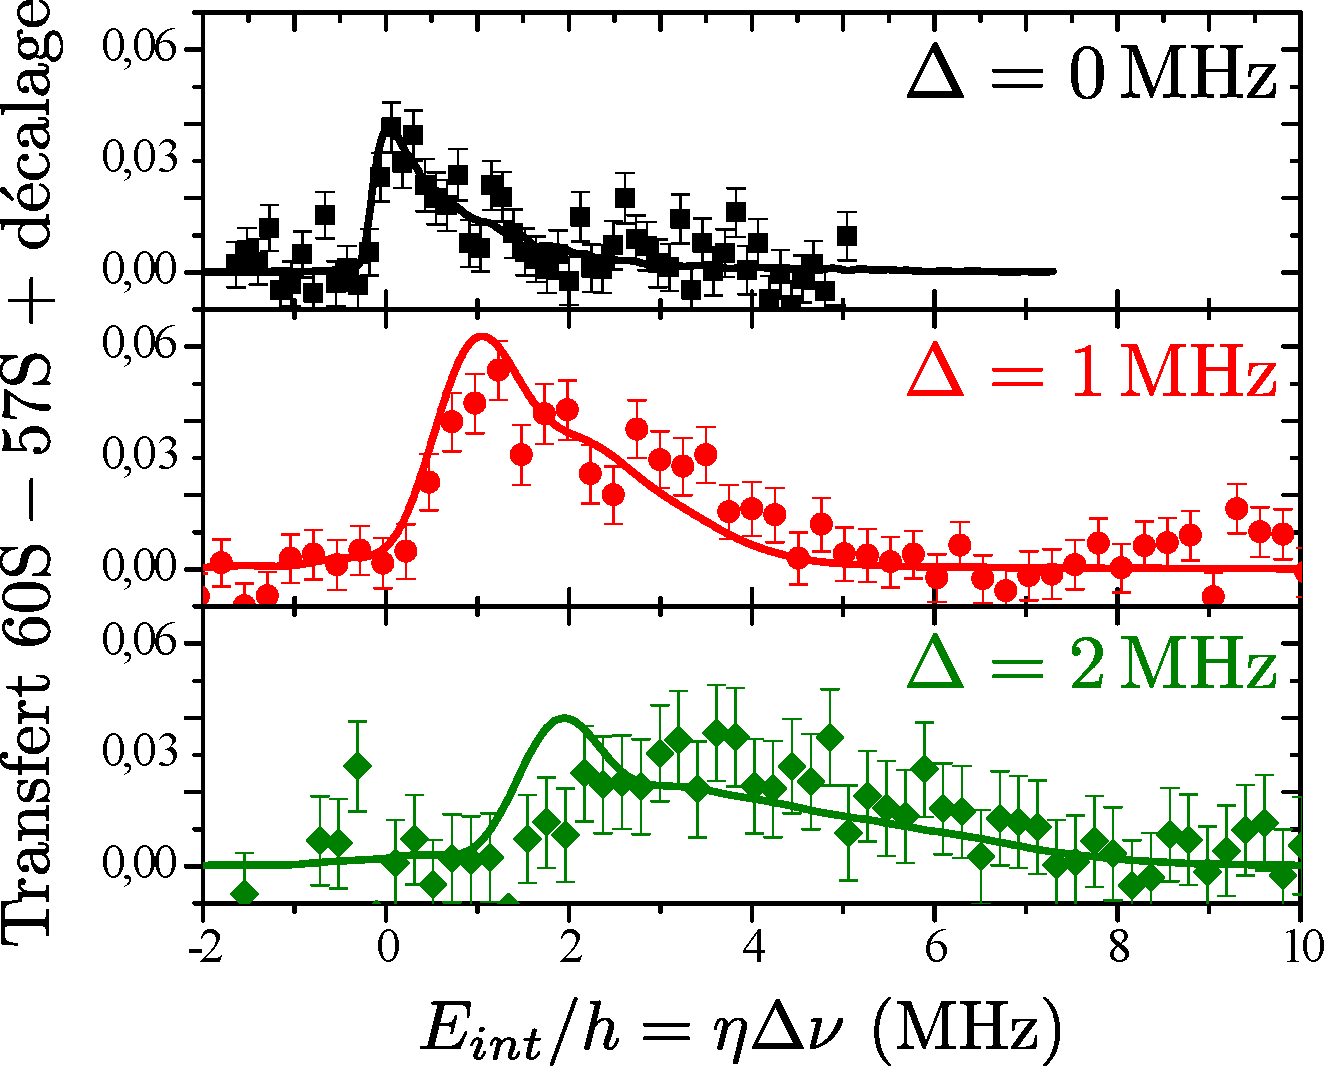
\includegraphics[width=.7\linewidth]{figures/low_l/micro_0delay_firstTest_Tigrane}
\caption[Comparaison des simulations aux spectres microonde immédiatement après excitation laser]{
Comparaison des simulations aux spectres microonde immédiatement après excitation laser.
Les spectres expérimentaux sont ceux de la figure \ref{fig:microwave_probe_0delay}.
Les lignes pleines sont les résultats de la simulation.
}
\label{fig:micro_0delay_firstTest}
\end{figure}
%
Malgré la simplicité du modèle numérique, l'accord avec l'expérience est raisonnable à ce stade.
Cela nous encourage à pousser plus loin la comparaison, en confrontant les simulations aux spectres microonde enregistrés au cours de l'explosion du nuage.

La figure \eqref{fig:microwave_explosion_firstSim} présente ces spectres, pour trois désaccords laser différents, comparés avec les simulations.
%
\begin{figure}[!h]
\centering
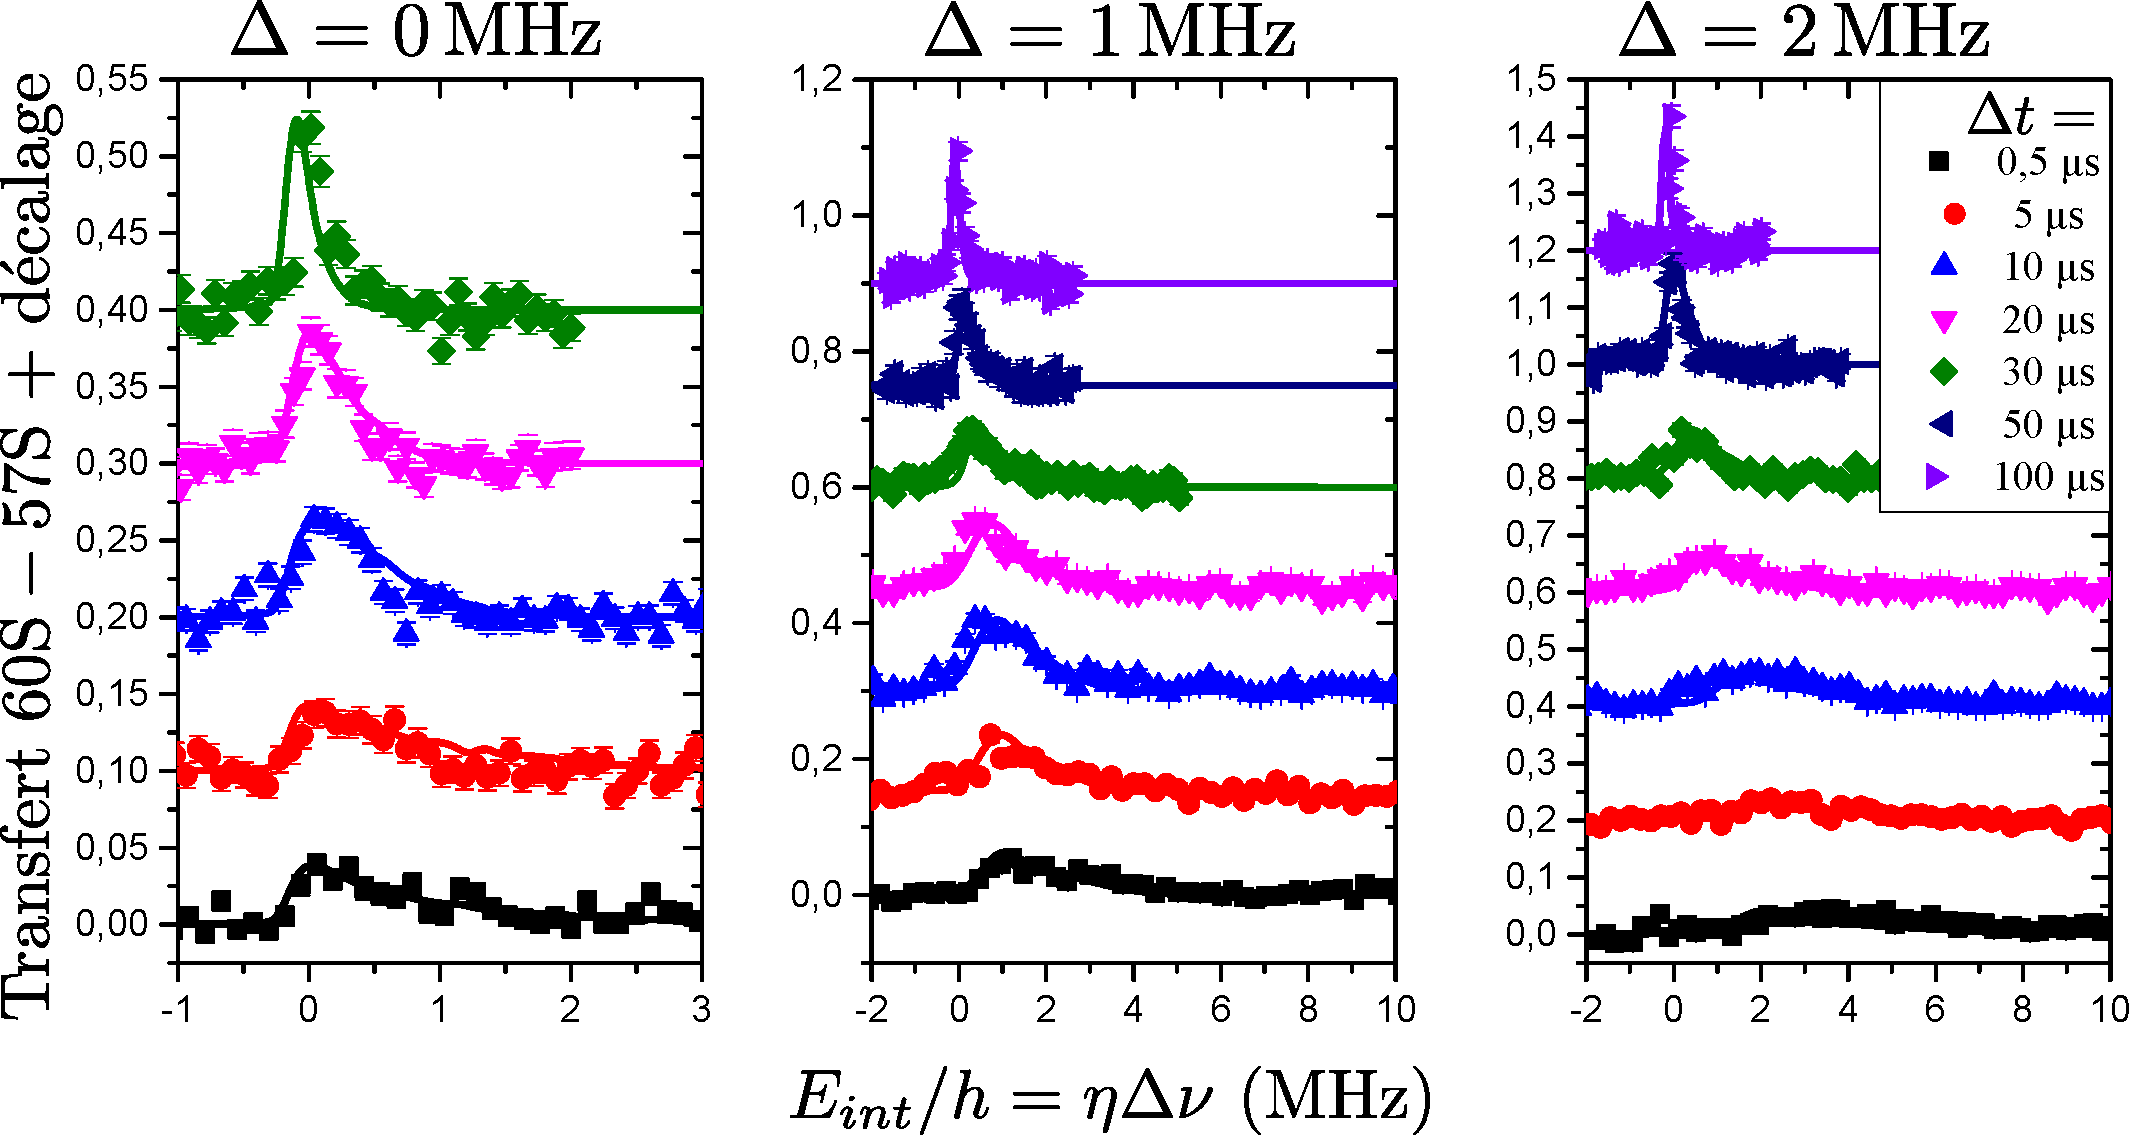
\includegraphics[width=\linewidth]{figures/low_l/expansion_012MHz_fisrtSim}
\caption[Comparaison des simulations aux spectres microonde lors de l'explosion du nuage]{
Comparaison des simulations aux spectres microonde lors de l'explosion du nuage, pour trois désaccords laser d'excitation $\Delta = \num{0}, \num{1}, \SI{2}{\MHz}$.
Les spectres expérimentaux sont ceux de la figure \ref{fig:microwave_explosion}.
Les lignes pleines sont les résultats de la simulation.
L'origine des axes verticaux de chacun des spectres est décalée et l'échelle des abscisses et des ordonnées de chacun des graphes est différente, par souci de visibilité.
}
\label{fig:microwave_explosion_firstSim}
\end{figure}
%
L'accord est ici aussi bon, confirmant la pertinence de notre modèle simple pour simuler l'explosion d'un nuage de Rydberg sous interaction.
\clearpage

\subsection{La limite du modèle : l'absence de temps}
\noindent Comme nous l'avons évoqué en \ref{subsec:algo_1}, ce modèle n'incorpore pas d'échelle de temps pour le processus d'excitation.
Cela pose la question de savoir comment simuler les spectres d'excitation laser.
En effet, on ne peut se permettre de fixer un nombre final d'atomes de Rydberg ici, car la simulation n'aurait plus de sens.
Nous avons tenté pour remédier à cela de faire correspondre un nombre d'itérations à la durée d'excitation 
%Une approche naïve de cette correspondance supposerait une relation linéaire, où le nombre d'atomes dont on teste la probabilité d'excitation serait proportionnel à la durée de l'impulsion laser.
%Cette hypothèse permet d'
de façon à intégrer le mouvement des atomes de Rydberg au cours même de l'excitation.%, ce qui est essentiel pour des durées d'impulsion supérieures à $\num{5}$ ou $\SI{10}{\us}$.
Pour cela, après chaque tirage au sort d'un atome, le mouvement du nuage de Rydberg est calculé sur la durée correspondant à une itération.

Les nombres d'itérations correspondant à chaque durée d'impulsion ont été choisis pour reproduire au mieux la queue à haute énergie des spectres, qui est due à une excitation facilitée à désaccord laser important.
La figure \ref{fig:opt_spectra_firstTest} présente les résultats des simulations ainsi menées, superposés aux résultats expérimentaux.
%
\begin{figure}[!h]
\centering
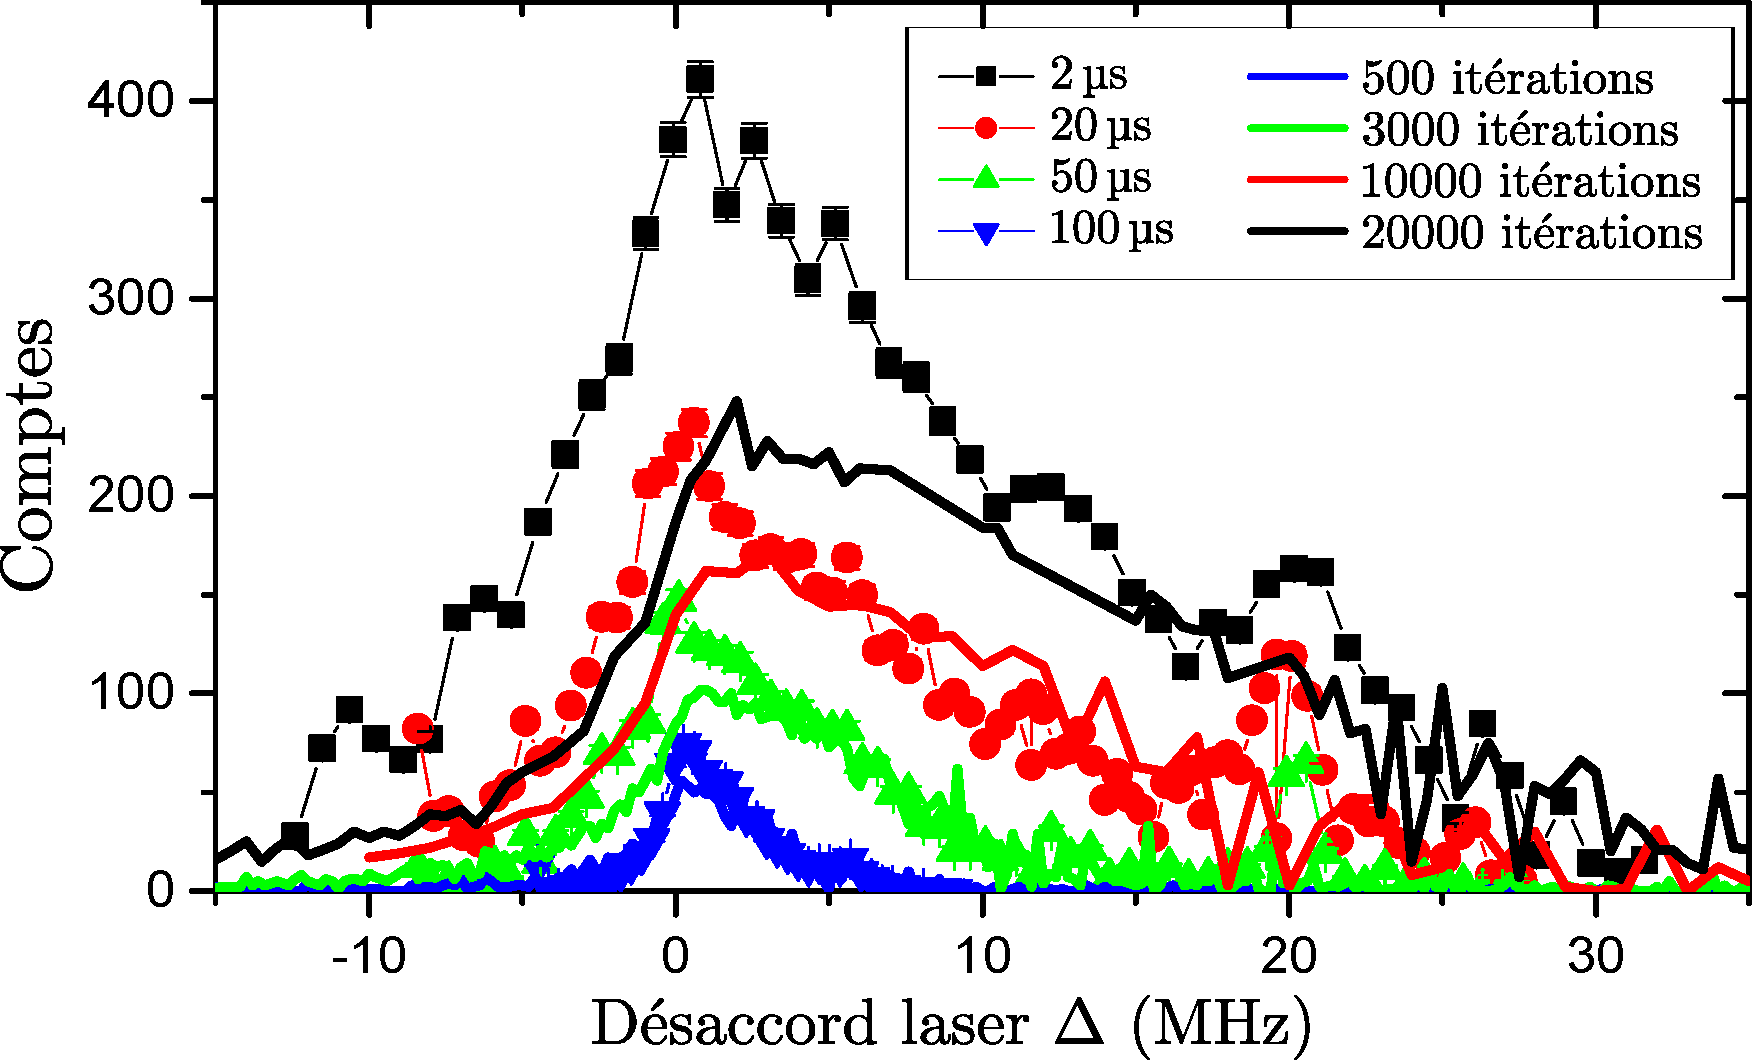
\includegraphics[width=\linewidth]{figures/low_l/raies_laser_vieilles_simus}
\caption[Comparaison des spectres optiques au premier modèle de simulation]{
Comparaison des spectres optiques aux simulations, pour différentes durées d'impulsion laser : $\SI{2}{},\SI{20}{},\SI{50}{}$ et $\SI{100}{\us}$.
Les spectres expérimentaux sont ceux de la figure \ref{fig:data_spectresoptiques}.
Les lignes pleines sont les résultats de la simulation.
Le nombre d'itérations de chaque simulation est choisi pour reproduire au mieux la queue à haute énergie des spectres expérimentaux.
Le calcul tient compte du mouvement des atomes de Rydberg durant l'excitation.
}
\label{fig:opt_spectra_firstTest}
\end{figure}
%
%La relation linéaire supposée entre le temps et le nombre d'itérations semble raisonnablement vérifiée.
%Un ajustement linéaire donne un rapport de $\SI{198}{} \pm \SI{5}{~} \text{itérations}/\si{\us}$.
%En revanche, 
Notre modèle sans échelle de temps explicite pendant l'excitation se montre incapable de reproduire les spectres expérimentaux d'excitation laser, et donc de rendre compte de la dynamique d'excitation de façon satisfaisante.
Il ne pourra ainsi pas être utilisé pour prédire les spectres d'excitation sous différentes conditions, si l'on souhaitait faire varier la densité atomique ou les paramètres d'impulsion laser.

Une seconde limite de ce modèle est l'absence de désexcitation stimulée des atomes de Rydberg sous l'effet du laser.
S'il y a suffisamment d'atomes dans l'état fondamental en résonance avec l'excitation, une telle désexcitation serait très vite compensée par une nouvelle excitation, ce qui autoriserait à omettre les processus de désexcitation.
Cependant à désaccord laser important, les régions résonantes d'excitation facilitée sont très proches des atomes de Rydberg déjà excités et le nombre d'atomes dans l'état fondamental que ces régions contiennent est limité par la densité atomique.
Les désexcitations d'atomes de Rydberg deviennent donc significatives dans le calcul du nombre final d'atomes de Rydberg et dans la configuration finale du nuage.

\clearpage
\section{Raffinement du modèle : équations de taux pour la dynamique d'excitation}
\noindent Face à l'incapacité de notre premier modèle à simuler l'excitation laser de façon satisfaisante, nous y avons introduit une échelle de temps.
Pour cela, la dynamique d'excitation est mise sous forme d'équations de taux pour chacun des atomes du nuage.
Un tel modèle a été proposé par l'équipe de M. Weidemüller \cite{MX_WEIDEMULLERRYDAGREGATES14} pour simuler des spectres optiques similaires à ceux que nous avons obtenus.
Nous avons ainsi établi un modèle combinant les deux aspects des équations de taux et de la prise en compte du mouvement des atomes de Rydberg durant l'excitation.
Le détail des équations de taux et de notre modèle numérique est discuté dans le chapitre 4 de la thèse de Thanh Long Nguyen \cite{PHD_NGUYEN}.
%Nous en ferons ici une présentation succincte, et comparerons les résultats obtenus aux spectres laser expérimentaux.
Après en avoir fait une présentation succincte, nous tenterons de le compléter avec la prise en compte d'un effet de chauffage du nuage atomique dû au laser rouge d'excitation.
Nous comparerons les résultats obtenus aux spectres expérimentaux, et extrairons des simulations certaines propriétés des nuages de Rydberg excités par des impulsions laser d'une durée inférieure à $\SI{20}{\us}$.
	
	\subsection{Modèle d'équation de taux et adaptation de l'algorithme}\label{subsec:rate_equation}
\noindent Notre modèle d'équation de taux repose sur les équations de Bloch optiques, prises dans la limite de grand déphasage, où les processus de dissipation sont dominés par un terme de déphasage.
Commençons par rappeler ces équations.

\subsubsection*{Équations de Bloch optiques à grand déphasage}
\noindent Les équations de Bloch optiques portent sur la matrice densité d'un atome à deux niveaux soumis à un champ laser.
Cette matrice densité peut s'écrire
\begin{equation}
\label{eq:density_matrix_Bloch}
\hat{\rho} = \bordermatrix{~ 	&\ket{g} 	& \ket{Ry} \cr
	\bra{g}		&\rho_{g,g}		&\rho_{g,Ry}	\cr 
	\bra{Ry} 		&\rho_{Ry,g}		&\rho_{Ry,Ry} \cr}
\end{equation}
où $\ket{g}$ représente l'état fondamental et $\ket{Ry}$ l'état excité de l'atome.
Les populations dans ces deux états sont respectivement $\rho_{g,g}$ et $\rho_{Ry,Ry}$.
La quantité $\rho_{g,Ry} = \rho_{Ry,g}^*$ représente la cohérence entre les états $\ket{g}$ et $\ket{Ry}$.

Les deux états atomiques sont distants en énergie d'une quantité $E_{Ry}-E_{g} = h\nu_{0} = \hbar\omega_0$.
La fréquence du laser sera notée $\nu =\omega/ 2\pi$.
En passant dans le référentiel tournant à la fréquence $\omega/2\pi$, par l'intermédiaire de l'opérateur d'évolution unitaire $\mathcal{U} = e^{i\omega t \ket{Ry}\bra{Ry}}$, les termes de population restent inchangés et les termes de cohérence deviennent $\tilde{\rho}_{g,Ry} = \tilde{\rho}_{Ry,g}^* =  \rho_{g,Ry}e^{i\omega t}$.
Dans ce référentiel, l'approximation séculaire permet de négliger les termes d'oscillation rapide en $\omega+\omega_0$, pour ne garder que les termes en $\omega-\omega_0 =\Delta$.
On obtient ainsi les équations suivantes d'évolution
\begin{equation}
\label{eq:Bloch_eq}
\left\{
\begin{aligned}
&\partial_t\rho_{Ry,Ry} = \mathrm{i} \frac{\Omega}{2} \left( \frac{}{}\! \tilde{\rho}_{Ry,g} - \tilde{\rho}_{g,Ry} \right) - \frac{1}{\tau}\rho_{Ry,Ry} \\
&\partial_t\tilde{\rho}_{g,Ry} =-\left( \frac{\gamma}{2} - \mathrm{i} \Delta \right) \tilde{\rho}_{Ry,g} + \mathrm{i} \frac{\Omega}{2} \left(\frac{}{}\! \rho_{Ry,Ry} - \rho_{g,g} \right),
\end{aligned}
\right.
\end{equation}
où $\Omega$ est la fréquence de Rabi, $\tau$ la durée de vie de l'état excité et $\gamma$ le taux de déphasage des cohérences.

La limite de grand déphasage consiste à considérer que
\begin{equation}
\label{eq:strong_dephasing}
\gamma \gg \Omega \gg 1/\tau,
\end{equation}
en se situant à des temps $t > \gamma^{-1}$.
Alors les cohérences atteignent leurs valeurs stationnaires et ainsi $\partial_t \tilde{\rho}_{g,Ry} \approx 0$.
En reprenant le système d'équations \eqref{eq:Bloch_eq} sous ces conditions, on obtient 
\begin{equation}
\label{eq:Bloch_approx}
\partial_t \rho_{Ry,Ry} = -\frac{(\Omega/2)^2 \gamma}{(\gamma/2)^2 + \Delta^2} \left(\frac{}{}\! \rho_{Ry,Ry} - \rho_{g,g} \right) - \frac{1}{\tau} \rho_{Ry,Ry}.
\end{equation}
On reconnaîtra ici une équation de taux équivalente au modèle des coefficients d'Einstein pour l'absorption, l'émission stimulée et l'émission spontanée de photons par un atome.
Le problème quantique de l'excitation de l'atome est réduit ici un problème stochastique classique avec un taux d'excitation $\Gamma_{exc}$ et de désexcitation $\Gamma_{de-exc}$ de l'atome valant
\begin{equation}
\label{eq:exc_de-exc_rate_1at}
\Gamma_{exc} = \frac{(\Omega/2)^2 \gamma}{(\gamma/2)^2 + \Delta^2} \hfill \text{et} \hfill
\Gamma_{de-exc} = \Gamma_{exc}+\frac{1}{\tau}. \hfill
\end{equation}
La généralisation à $N$ atomes de Rydberg se fait en tenant compte des interactions entre eux.
Pour chaque atome de Rydberg $i$, il conviendra de déduire du désaccord laser son énergie d'interaction $E_{int}(i)$ avec les atomes de Rydberg déjà présents.
Les taux d'excitation et de désexcitation pour l'atome $i$ deviennent :
\begin{equation}
\label{eq:exc_de-exc_rate_atomi}
\Gamma_{exc}(i) = \frac{(\Omega/2)^2 \gamma}{(\gamma/2)^2 + (\Delta - E_{int}(i))^2} \hfill \text{et} \hfill
\Gamma_{de-exc}(i) = \Gamma_{exc}(i)+\frac{1}{\tau}, \hfill
\end{equation}
où $E_{int}(i) = \sum_{j\neq i} C_6/r_{ij}^6$, la somme portant sur tous les atomes de Rydberg $j$ déjà présents.

Afin d'appliquer ces équations de taux à notre système, il est nécessaire d'estimer le taux de déphasage $\gamma$.
L'équation \eqref{eq:Bloch_approx}, établie pour un atome unique, reste valide dans le cas d'un nuage de Rydberg dilué, où les interactions dipolaires sont négligeables.
L'hypothèse \eqref{eq:strong_dephasing} permet de vérifier la condition $\Gamma_{exc} \gg 1/\tau$, donc de négliger la désexcitation spontanée aux temps courts.
La résolution de l'équation \eqref{eq:Bloch_approx} dans ces conditions et avec tous les atomes initialement dans l'état fondamental donne la solution 
\begin{equation}
\label{eq:Lorenztian_rhorr}
\rho_{Ry,Ry} (t) = \frac{1}{2}\left( 1-e^{-2\Gamma_{exc}t} \right)
\underset{\Gamma t \ll 1}{\simeq} \Gamma_{exc} t = \frac{(\Omega/2)^2 \gamma}{(\gamma/2)^2 + \Delta^2} \cdot t.
\end{equation}
La population dans l'état excité est donc répartie sur un spectre lorentzien de largeur à mi-hauteur $\gamma$.
Cela nous permet d'identifier le taux de déphasage des équations de Bloch à la largeur de raie $\gamma = \SI{626}{\kHz}$ du spectre de référence en nuage dilué de la figure \eqref{fig:data_spectresoptiques}.

	\subsubsection*{Fonctionnement de l'algorithme}
\noindent Il nous est désormais possible d'inclure une échelle de temps à notre algorithme de simulation, sous la forme des taux d'excitation et de désexcitation donnés par l'équation \eqref{eq:exc_de-exc_rate_atomi}.
Au lieu de tirer au sort un atome à chaque étape, le calcul de l'excitation nécessite désormais de calculer les taux $\Gamma_{exc}(i)$ et $\Gamma_{de-exc}(i)$ à chaque pas de temps et pour chaque atome du nuage, qu'il soit dans l'état fondamental ou dans l'état excité.
Le détail de l'algorithme est expliqué dans la thèse de Thanh Long Nguyen \cite{PHD_NGUYEN}, et présenté en annexe \ref{app:algo}.

Quelques spécificités de cette nouvelle version méritent d'être discutées ici.
En premier lieu, le choix d'exciter ou non un nouvel atome de Rydberg ne peut se faire uniquement d'après le calcul de son taux d'excitation $\Gamma_{exc}(i)$.
En effet, cela amènerait à exciter plusieurs atomes de Rydberg lors du même pas de temps, qui ne respecteraient pas la dynamique d'excitation imposée par les interactions dipolaires.
Par exemple, à désaccord laser nul, deux atomes pourraient être excités dans la même sphère de blocage, ce qui est interdit par le mécanisme de blocage dipolaire.

\`A chaque pas de temps, les atomes sélectionnés d'après leur taux d'excitation sont ainsi placés dans une liste \mcal{L} de \og candidats \fg{}.
Cette liste est ensuite aléatoirement réordonnée et son premier élément est excité.
Pour chacun des éléments suivants un nouveau taux d'excitation est calculé, qui vaut
\begin{equation}
\tilde{\Gamma}_{exc}(i) = \frac{(\Omega/2)^2 \gamma}{(\gamma/2)^2 + (\Delta - \tilde{E}_{int}(i))^2},
\end{equation}
avec
\begin{equation}
\tilde{E}_{int}(i) = \sum_{j} C_6/r_{ij}^6,
\end{equation}
où la somme est faite sur les atomes $j$ appartenant à la liste de candidats \mcal{L} et qui ont été excités.
L'excitation de l'atome $i$ est décidée en fonction de ce nouveau taux.
Cette étape permet de respecter les contraintes interactionnelles de l'excitation à l'intérieur d'un même pas de temps.

Certains paramètres de simulation sont désormais exprimés différemment.
La puissance des laser est prise en compte par un paramètre $\Omega_0$ de fréquence de Rabi au centre des faisceaux laser, de même que la largeur spectrale $\gamma$ d'excitation à un atome.
Le faisceau laser bleu présente une bande latérale à $\SI{20}{\MHz}$, en raison du dispositif de verrouillage de la cavité de doublage de fréquence.
Cette bande latérale est prise en compte dans les simulations, en ajoutant au taux d'excitation des atomes un terme désaccordé de $\SI{20}{\MHz}$ et pondéré par un facteur d'amplitude $x_{20}$ sur la fréquence de Rabi.
L'extension spatiale du piège dans chacune des trois directions est calculée à partir de la fréquence de piégeage dans cette direction, elle-même mesurée expérimentalement, et de la température initiale $T_0$ du nuage.
Nous pourrons ainsi utiliser la température du nuage atomique comme paramètre explicite de simulation.
%et intégrer au calcul un processus de chauffage dû au laser rouge, tel qu'évoqué en \ref{subsec:2photon_excite}.

\newpage
\subsection{Résultats simulant une expansion du nuage atomique}\label{subsec:bigsigma}
\noindent Les simulations présentées dans la thèse de Thanh Long Nguyen \cite{PHD_NGUYEN} ont permis de reproduire les spectres d'excitation laser, pour toutes les durées d'impulsion, à la condition d'imposer une température du nuage atomique différente pour chaque durée d'impulsion.
La température étant ici prise en compte uniquement comme paramètre de l'extension spatiale du piège, la reproduction des données expérimentales nécessitait en réalité d'adapter la taille du piège à chaque durée d'impulsion.

%Les spectres simulés et expérimentaux, ainsi que la température optimale pour chaque durée d'impulsion laser, sont représentés en figure \ref{fig:Temp_fit_spectres_TL}.
%
%\begin{figure}[h]
%\centering
%%\includegraphics[scale=•]{•}
%graphe températures TLN
%\caption[]{}
%\label{fig:Temp_fit_spectres_TL}
%\end{figure}
%
%L'interprétation la plus évidente d'une augmentation de la taille du nuage au cours d'une impulsion laser est la présence d'un processus de chauffage.
%%e la nécessité d'augmenter la température du piège avec la durée d'impulsion laser, est la présence d'un processus de chauffage du nuage d'atomes dans l'état fondamental.
%%De plus, l'ordre de grandeur de ce \og chauffage \fg{} est compatible avec l'effet du laser rouge d'excitation mentionné en \ref{subsec:2photon_excite}.
%La source de chauffage la plus évidente est l'absorption et la ré-émission de photons rouge par les atomes dans l'état fondamental.
%Nous avons alors souhaité intégrer ce chauffage directement à la dynamique d'excitation, afin d'estimer de façon réaliste son effet sur la taille du nuage atomique et sur l'excitation du nuage d'atomes de Rydberg.
%, pour deux raisons.
%La première est que cela permet de limiter le nombre de paramètres d'ajustement, en n'imposant qu'une seule température du nuage atomique.
%La seconde est que l'excitation avec une température qui varie au cours du temps peut avoir une dynamique différente de l'excitation à température fixe.

Cependant, rien ne justifie que les conditions initiales de température, ou de taille du nuage, dépendent de la durée d'impulsion laser.
Nous avons donc souhaité intégrer directement au calcul un accroissement de la taille du nuage au cours de l'excitation.

Nous appliquons un modèle simple, où la taille du nuage évolue dans les trois directions comme
\begin{equation}
\sigma^2(t) = \sigma^2 (t=0) \cdot \left( \frac{}{} \! 1 + Dt \right),
\end{equation}
où $\sigma$ est le rayon gaussien du nuage, $t$ le temps et $D$ un coefficient d'expansion.
Cela permet de reproduire de façon satisfaisante les spectres expérimentaux, comme le montre la figure \eqref{fig:fitsim_spectresoptiques_0830126}, avec les paramètres de simulation résumés en table \eqref{tab:fit_sim_bigsigma}.

L'accord de ce modèle de simulation avec les données expérimentales est excellent pour les durées d'impulsions de $\SI{2}{},\SI{20}{}$ et $\SI{50}{\us}$.
Le spectre à $\SI{100}{\us}$ est très bien reproduit pour les désaccords laser supérieurs à $\SI{5}{\MHz}$.

Les paramètres d'ajustement sont la température initiale du nuage, qui a un effet très important sur les spectres, la fréquence de Rabi $\Omega_0$ au centre des faisceaux laser, l'amplitude de bande latérale $x_{20}$ et le coefficient d'expansion $D$.
La fréquence de Rabi et la température initiale sont ajustées sur le spectre à $\SI{2}{\us}$ uniquement.
L'amplitude de bande latérale $x_{20}$ est ajustée sur le spectre à $\SI{20}{\us}$.
L'écart entre la fréquence de Rabi calculée à partir des puissances et des géométries des faisceaux lasers et la fréquence de Rabi simulée est très important.
Nous attribuons cela à la mauvaise transmission des faisceaux laser à travers les hublots d'accès optique du cryostat.
En effet, nous avons constaté un dépôt de gaz résiduel ou de graisse sur les hublots froids de la jupe d'azote.
L'effet de ce dépôt est difficile à évaluer, car celui-ci disparaît dès que les hublots sont réchauffés à température ambiante.
Un tel dépôt a été observé sur d'autres expériences en environnement cryogénique \cite{PHD_LEUPOLD_ETHZ}.

Le coefficient d'expansion $D$ est ajusté de façon à obtenir le meilleur accord pour toutes les durées d'impulsion, en particulier $\SI{50}{}$ et $\SI{100}{\us}$ qui y sont plus sensibles.
Le coefficient optimisé $D = \SI{1.575e-2}{\per\us}$ permet de reproduire les données expérimentales.
Quel phénomène peut expliquer cette expansion du nuage ?
L'interprétation la plus évidente d'une augmentation de taille du nuage est la présence d'un processus de chauffage.
 
\begin{figure}[h]
\centering
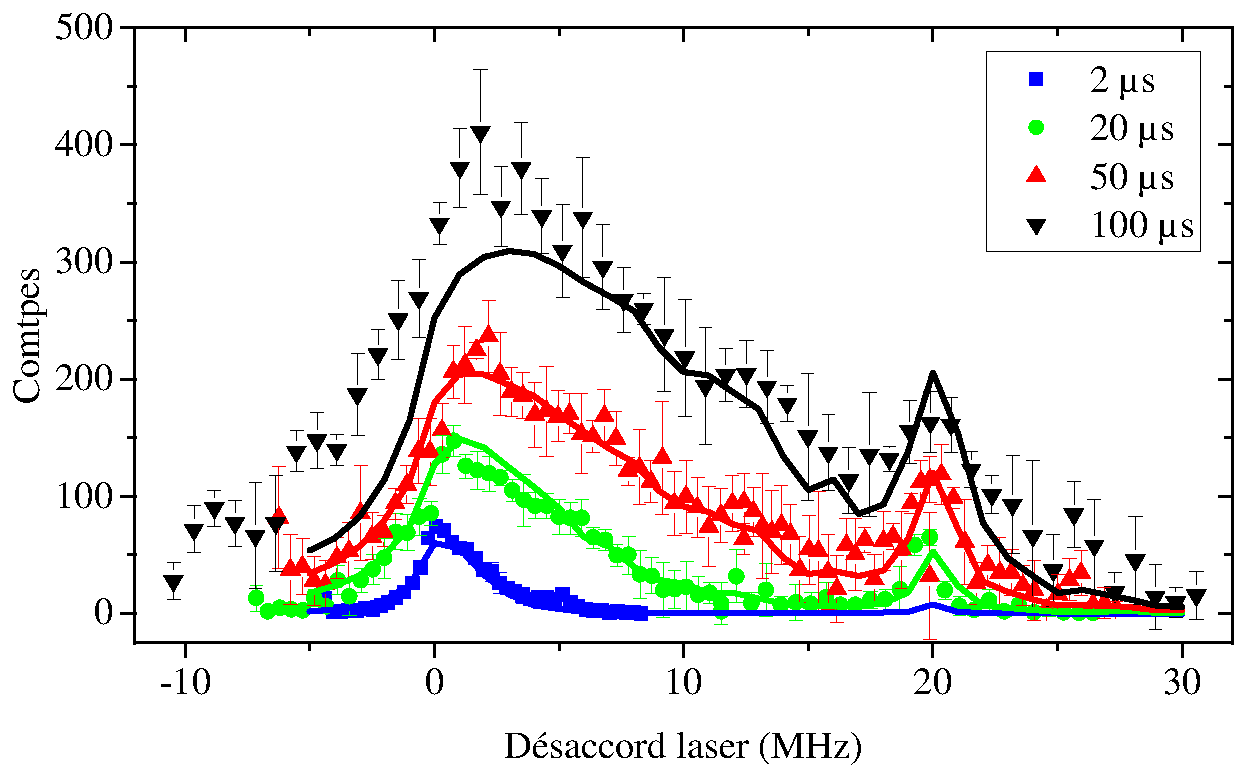
\includegraphics[width=\linewidth]{figures/low_l/fitsim_spectresoptiques_0830126}
\caption[Comparaison des spectres optiques aux simulations avec équations de taux]{
Comparaison des spectres optiques aux simulations, pour différentes durées d'impulsion laser : $\SI{2}{},\SI{20}{},\SI{50}{}$ et $\SI{100}{\us}$.
Les spectres expérimentaux sont ceux de la figure \ref{fig:data_spectresoptiques}.
Les lignes pleines sont les résultats de la simulation.
%Le calcul tient compte du mouvement des atomes de Rydberg durant l'excitation.
%Les traits pointillés sont les résultats des simulations sans tenir compte de l'effet de chauffage du nuage atomique.
Le modèle simule une expansion importante du nuage atomique pendant l'excitation.
}
\label{fig:fitsim_spectresoptiques_0830126}
\end{figure}

\begin{table}[h]
	\centering
	\caption[Paramètres de simulation]{Valeurs expérimentales et de simulation des paramètres d'excitation des spectres.
	}
	\label{tab:fit_sim_bigsigma}
	\begin{tabular}{l c c}
		\toprule\midrule
		Paramètres fixes &	Valeur expérimentale & Valeur de simulation\\		
		\midrule
		Fréquence de piégeage $f_x$ & \SI{47}{\Hz} & \SI{47}{\Hz} \\
		Fréquence de piégeage $f_y$ & \SI{244}{\Hz} & \SI{244}{\Hz} \\
		Fréquence de piégeage $f_z$ & \SI{262}{\Hz} & \SI{262}{\Hz} \\
		Nombre d'atomes $N$ & $\SI{12000}{}\pm\SI{2000}{}$ & $\SI{12000}{}\pm\SI{2000}{}$ \\
		Col du laser bleu $w_{480}$ & \SI{22}{\um} & \SI{22}{\um} \\
		Col du laser rouge $w_{780}$ & \SI{150}{\um} & $\infty$ \\
		Largeur de raie $\gamma$ & \SI{626}{\kHz} & \SI{626}{\kHz}\\
%		Taux de chauffage $\partial _t T$ & \SI{12.6}{\nano\K/\us} & \SI{12.6}{\nano\K/\us} \\
		\midrule
		Paramètres d'ajustement & &\\\midrule
		Amplitude de bande latérale $x_{20}$ & non mesurée & \SI{0.12}{} \\
		Fréquence de Rabi max. $\Omega_0/(2\pi)$ & \SI{296}{\kHz} & $\SI{60}{} \pm \SI{5}{\kHz}$\\
		Température initiale $T_0$ & $\SI{0.6}{}\pm\SI{0.3}{\uK}$ & $\SI{0.8}{}\pm\SI{0.05}{\uK}$\\
		Coefficient d'expansion $D$ & inconnu & $\SI{1.575e-2}{\per\us}$\\
		\midrule
		\bottomrule
 	\end{tabular}
\end{table}

\clearpage
\subsection{Chauffage et expansion réalistes du nuage atomique}
\noindent Comme nous l'avions évoqué en \ref{subsec:2photon_excite}, l'absorption et la ré-émission par les atomes du seul laser rouge d'excitation est responsable d'un chauffage du nuage.
Cela semble, au premier abord, être une explication plausible de l'expansion du nuage atomique.

Les photons rouges absorbés ont pour effet de pousser l'ensemble du nuage le long de la direction de propagation des lasers, ce qui n'engendre pas de chauffage mais seulement un déplacement.
La ré-émission spontanée des photons rouges par les atomes peut être traitée comme une marche aléatoire discrète.
La taille des pas de cette marche est l'impulsion de recul $\Delta p=\hbar k$ reçue par l'atome dans une direction aléatoire lors de l'émission, où $k$ est le vecteur d'onde du photon.
Le taux de répétition de ce processus est donné par le taux d'émission spontanée $\Gamma_{sp}$, discuté au chapitre \ref{chapter:setup_coldatoms_Rydberg}, et qui vaut
\begin{equation}
\label{eq:Gamma_sp}
\Gamma_{sp} \simeq \frac{\Omega_r^2}{2\delta^2}\Gamma,
\end{equation}
où $\Omega_r$ et $\delta$ sont respectivement la fréquence de Rabi et le désaccord du laser rouge sur la transition $\ket{\mathrm{5S_{1/2},F=2,m_F=+2}} \rightarrow \ket{\mathrm{5P_{3/2},F'=3,m_F'=+3}}$, et $\Gamma$ est la largeur naturelle de celle-ci.
La variance de la quantité de mouvement des atomes évolue ainsi comme
\begin{equation}
\label{eq:momentum_randomwalk}
\braket{p^2 (t)} = \braket{p^2(t=0)} + (\hbar k)^2 \cdot \Gamma_{sp}t
\end{equation}
et donc la température du nuage évolue comme 
\begin{equation}
\label{eq:heating_randomwalk}
T(t) = \frac{\braket{p^2 (t)}}{3m\kb} =
T(t=0) + \frac{(\hbar k)^2}{3m\kb} \Gamma_{sp} t
=T(t=0) + \partial_t T \times t~.
\end{equation}

Avec les paramètres du laser rouge donnés au chapitre \ref{chapter:setup_coldatoms_Rydberg}, soit $\Omega_r = 2\pi\times \SI{40}{\MHz}$ et $\delta=2\pi\times\SI{540}{\MHz}$, nous obtenions un taux d'émission spontanée $\Gamma_sp = 2\pi\times\SI{16.6}{\kHz}$.
Ainsi, un atome absorbe et ré-émet un photon rouge toutes les $\Gamma_{sp}^{-1}=\SI{9.565}{\us}$.
L'émission d'un photon de longueur d'onde $\lambda=\SI{780}{\nano\metre}$ transfère à un atome une impulsion de recul $\hbar k = h/\lambda = \SI{8.5e-28}{\kg\m\per\s}$.
Nous obtenons alors un taux de chauffage $\partial_t T = \SI{12.6}{\nano\K/\us}$, de même qu'au chapitre \ref{chapter:setup_coldatoms_Rydberg}.

Ce taux de chauffage peut-il expliquer l'expansion du nuage atomique avec le coefficient d'expansion $D$ que nous avons obtenu en ajustant les paramètres de simulation ?
Les nuages atomiques que nous excitons sont soumis à ce chauffage pendant une durée de $\SI{100}{\us}$ au maximum.
Après une telle durée, un nuage dont la température initiale était de $\SI{0.8}{\uK}$ aura été chauffé à une température de $\SI{0.8}{\uK}+\SI{100}{\us}\times\partial_t T = \SI{2.06}{\uK}$.
Cependant, un temps de $\SI{100}{\us}$ est loin d'être suffisant pour que la taille du nuage atomique piégé atteigne sa valeur d'équilibre thermique $\sigma=\sqrt{\kb T /m(2\pi f)^2}$, où $f$ est la fréquence de piégeage.
En effet, le temps caractéristique pour atteindre cet équilibre est donné par l'inverse de la fréquence de piégeage.
Or ici, les fréquences de piégeage sont de $\SI{47}{},\SI{244}{}$ et $\SI{262}{\Hz}$ dans les directions $x,y$ et $z$ respectivement.
La taille d'équilibre du nuage atomique imposée par sa température ne peut donc être atteinte qu'après plusieurs millisecondes.

Afin d'estimer de façon réaliste l'effet du chauffage sur le nuage atomique, nous avons simulé la dynamique des atomes dans l'état fondamental soumis aux processus d'émission spontanée responsables du chauffage.
Cette simulation calcule les trajectoires des $\SI{12000}{}$ atomes du nuage en fonction du temps, en tenant compte de leur distribution de vitesse initiale, et des événements aléatoires d'absorption et émission spontanée d'un photon rouge.
Les atomes sont considérés comme indépendants les uns des autres, et la probabilité d'absorber et ré-émettre un photon rouge est représentée par le taux $\Gamma_{sp}$ de l'équation \eqref{eq:Gamma_sp}.
Le résultat de cette simulation pour l'extension spatiale du piège selon $y$ est représentée en figure \eqref{fig:sigma_real_heat}.

\begin{figure}[h]
\centering
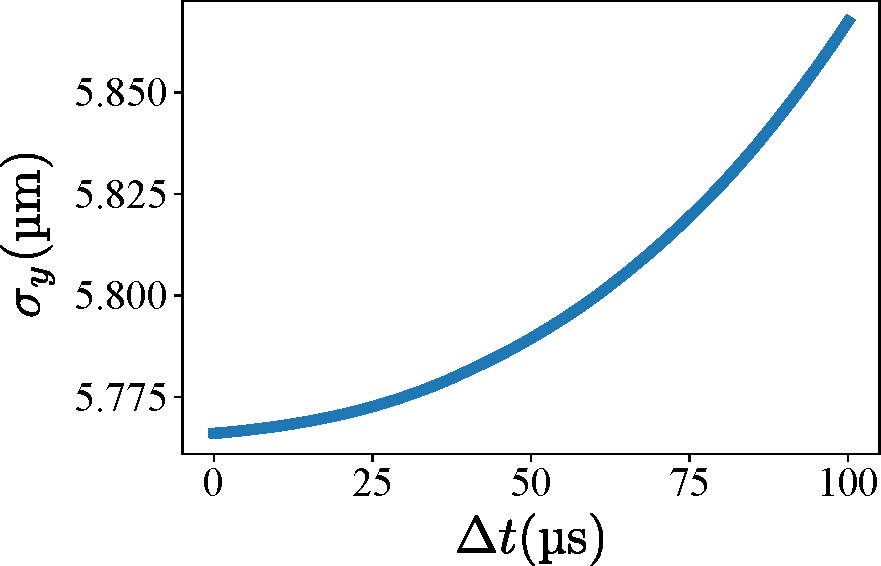
\includegraphics[width=0.6\linewidth]{figures/low_l/sigmaytime}
\caption[Évolution de la taille du nuage sous l'effet du chauffage dû au laser rouge]{
Évolution de la taille du nuage sous l'effet du chauffage dû au laser rouge.
La courbe représente le rayon gaussien $\sigma_y$ du nuage atomique selon la direction $y$, en fonction de la durée d'impulsion laser $\Delta t$.
Les photons rouges sont absorbés et ré-émis à un taux $\Gamma_{sp}$ estimé à $2\pi\times\SI{16.6}{\kHz}$.
}
\label{fig:sigma_real_heat}
\end{figure}

L'effet du chauffage sur la taille du nuage atomique pour une durée d'impulsion laser de $\SI{100}{\us}$ reste très limité : l'extension spatiale transverse $\sigma_y$ augmente de moins de $\SI{2}{\percent}$.
La même simulation montre que, pour atteindre les tailles de nuage correspondant aux températures optimales simulées par Thanh Long Nguyen \cite{PHD_NGUYEN}, il faudrait un taux de chauffage au minimum $\SI{100}{}$ fois plus important.
% afin d'atteindre les tailles de nuage permettant un bon accord des spectres optiques simulés avec les données expérimentales.

%En intégrant directement les trajectoires des atomes dans l'état fondamental à la simulation de l'excitation, nous avons pu confirmer le peu d'effet, sur les spectres optiques, du chauffage dû au laser rouge.

%
%
%
%
%
%----------------------------------------
%\noindent Lors de l'excitation à deux photons du niveau de Rydberg $\mathrm{60S}$, les atomes du nuage absorbent des photons rouges à $\SI{780}{\nano\meter}$.
%Si l'atome qui absorbe un photon rouge n'absorbe pas de photon bleu, c'est-à-dire s'il n'est pas excité au niveau de Rydberg, alors il réémettra le photon rouge.
%Cela mène à un chauffage du nuage atomique, caractérisé par deux grandeurs :
%le taux d'émission spontanée $\Gamma_{sp}$ des photons rouges par les atomes et la variation de température $\Delta T_{\text{1photon}}$ causée par l'émission spontanée d'un photon.
%
%Le calcul du taux d'émission spontanée est discuté en \ref{subsec:2photon_excite} et aboutit à l'équation \eqref{eq:scattering_5P3/2} :
%\begin{equation}
%\label{eq:Gamma_sp}
%\Gamma_{sp} \simeq \frac{\Omega_r^2}{2\delta^2}\Gamma,
%\end{equation}
%où $\Omega_r$ et $\delta$ sont respectivement la fréquence de Rabi et le désaccord du laser rouge sur la transition $\ket{\mathrm{5S_{1/2},F=2,m_F=+2}} \rightarrow \ket{\mathrm{5P_{3/2},F'=3,m_F'=+3}}$, et $\Gamma$ est la lergeur naturelle de celle-ci.
%
%Le processus d'émission spontanée de photons rouges induit une variation de la quantité de mouvement des atomes du nuage, qui parcourt une marche aléatoire.
%Cette marche aléatoire a pour paramètres la taille $\Delta p$ d'un pas dans l'espace des quantités de mouvement, égale à l'impulsion de recul due à l'émission d'un photon, et le taux de répétition de ces pas, qui vaut $\Gamma_{sp}$.
%L'effet de la marche aléatoire est une augmentation au cours du temps de la variance $\braket{p^2}$.
%Chaque pas de la marche fait croître cette variance d'une quantité $(\Delta p)^2$, où $\Delta p = \hbar k$ est la quantité de mouvement du photon émis, avec $k$ la norme de son vecteur d'onde.
%En supposant une distribution de Maxwell-Boltzmann des vitesses au sein du nuage atomique, on en déduit que l'émission d'un photon cause une augmentation de température pour un atome de
%\begin{equation}
%\label{eq:heating_1photon}
%\Delta T_{\text{1photon}} = \frac{(\Delta p)^2}{3m\kb} = \frac{(\hbar k)^2}{3m\kb}
%\end{equation}
%
%Ce processus étant répété avec un taux $\Gamma_{sp}$, on peut exprimer la variance de la quantité de mouvement en fonction du temps $t$ par
%\begin{equation}
%\label{eq:momentum_randomwalk}
%\braket{p^2 (t)} = \braket{p^2(t=0)} + (\hbar k)^2 \cdot \Gamma_{sp}t
%\end{equation}
%ou, de façon équivalente, une température qui varie comme
%\begin{equation}
%\label{eq:heating_randomwalk}
%T(t) = T(t=0) + \Delta T_{\text{1photon}}\Gamma_{sp}t = \frac{\braket{p^2 (t)}}{3m\kb} =
%T(t=0) + \frac{(\hbar k)^2}{3m\kb} \Gamma_{sp} t.
%\end{equation}
%
%En fin de compte, nous pouvons rendre compte du processus de chauffage du nuage atomique par un taux de chauffage
%\begin{equation}
%\label{eq:heating_rate}
%\partial_t T = \frac{(\hbar k)^2}{3m\kb} \cdot \frac{\Omega_r^2}{2\delta^2} \cdot \Gamma.
%\end{equation}
%Dans les conditions de nos expériences, avec un laser à $\SI{780}{\nano\meter}$, une largeur de raie $\Gamma = 2\pi\times \SI{6.065}{\MHz}$, une fréquence de Rabi du rouge $\Omega_r = 2\pi\times \SI{40}{\MHz}$ et un désaccord de $\delta = 2\pi \times \SI{540}{\MHz}$, nous obtenons un taux de chauffage estimé, comme en \ref{subsec:2photon_excite}, à
%\begin{equation}
%\label{heating_rate_value}
%\partial_t T \simeq \SI{12.6}{\nano\K / \micro\second}.
%\end{equation}
%
%\subsubsection*{Conséquences du chauffage sur la taille du nuage atomique}
%%et implémentation dans le modèle de simulation}
%\noindent La conséquence de ce chauffage pour la dynamique d'excitation réside dans l'accroissement de la taille du nuage atomique au cours du temps.
%En effet, l'effet Doppler dû à une température de l'ordre de $\SI{1}{\micro\kelvin}$ est au maximum de $\Delta \nu_{max} \sim \SI{42}{kHz}$ sur la transition $\mathrm{5S-60S}$.
%Cela étant très inférieur à la largeur de raie $\gamma$, l'effet Doppler est tout à fait négligeable. % malgré le chauffage.
%
%Un nuage atomique piégé dans un piège harmonique présente une distribution gaussienne de densité.
%Son extension, à l'équilibre thermique, est directement liée à la température par l'intermédiaire des fréquences de piégeage $f_{x,y,z}$ dans chaque direction :
%\begin{equation}
%\label{eq:trap_size_temp}
%\sigma_{x,y,z} = \sqrt{\frac{m\kb T}{(2\pi f_{x,y,z})^2}}.
%\end{equation}
%
%Une première approche consisterait à recalculer, au fur et à mesure qu'augmente la température du nuage, son extension spatiale d'après l'équation \eqref{eq:trap_size_temp}.
%On obtiendrait alors un gonflement du nuage au cours du temps :
%\begin{equation}
%\label{eq:bigsigma_t}
%\sigma(t) = \sigma_0\times\sqrt{T(t)/T_0} = \sigma_0\times\sqrt{1+t\cdot\partial_t T},
%\end{equation}
%où $\sigma_0$ et $T_0$ sont l'extension du nuage et sa température à l'instant initial $t=0$.
%Cependant, cette évolution de taille du nuage n'est valide que si, à chaque instant, le profil de densité du nuage est à l'équilibre thermique.
%Or, le temps caractéristique nécessaire pour atteindre cet équilibre est de l'ordre de l'inverse des fréquences de piégeage $f_{x,y,z}$ et est donc de l'ordre de quelques $\SI{}{\ms}$.
%Les durées qui nous intéressent étant au maximum de $\SI{0.1}{\ms}$, il est raisonnable de supposer que cet équilibre n'est pas atteint.
%
%Afin d'estimer de façon plus réaliste l'effet du chauffage sur le nuage atomique, nous avons simulé la dynamique des atomes dans l'état fondamental soumis aux processus d'absorption et d'émission spontanée responsables du chauffage.
%Cette simulation calcule les trajectoires des $\SI{12000}{}$ atomes du nuage en fonction du temps, en tenant compte de leur distribution de vitesse initiale, et des événements aléatoires d'absorption et émission spontanée d'un photon rouge.
%Les atomes sont considérés comme indépendants les uns des autres, et la probabilité d'absorber et ré-émettre un photon rouge est représentée par le taux $\Gamma_{sp}$ de l'équation \eqref{eq:Gamma_sp}.
%Le résultat de cette simulation pour l'extension spatiale du piège selon $y$ est représentée en figure \eqref{fig:sigma_real_heat}.
%%
%\begin{figure}[h]
%\centering
%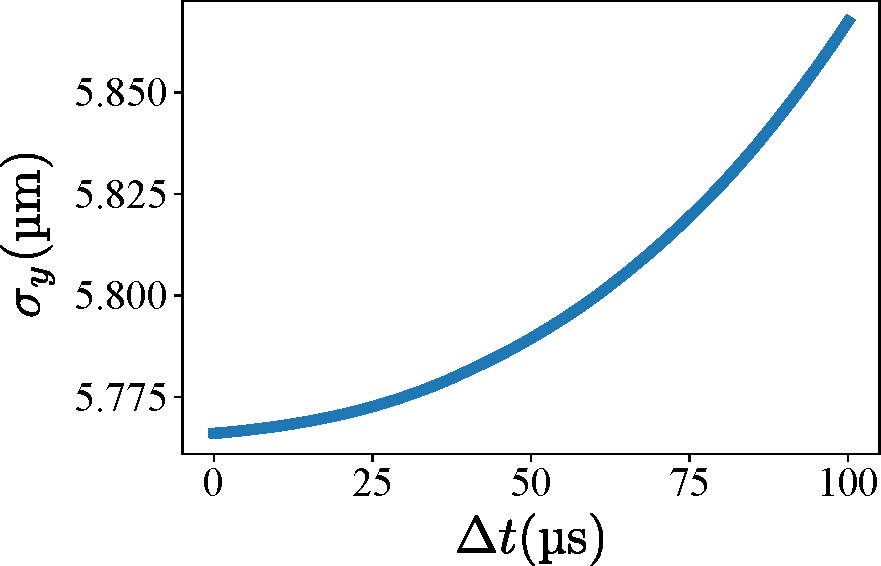
\includegraphics[width=0.6\linewidth]{figures/low_l/sigmaytime}
%\caption[Évolution de la taille du nuage sous l'effet du chauffage dû au laser rouge]{
%Évolution de la taille du nuage sous l'effet du chauffage dû au laser rouge.
%La courbe représente le rayon gaussien $\sigma_y$ du nuage atomique selon la direction $y$, en fonction de la durée d'impulsion laser $\Delta t$.
%Les photons rouges sont absorbés et ré-émis à un taux $\Gamma_{sp}$ estimé à $2\pi\times\SI{16.6}{\kHz}$.
%}
%\label{fig:sigma_real_heat}
%\end{figure}
%%
%L'effet du chauffage sur la taille du nuage atomique pour une durée d'impulsion laser de $\SI{100}{\us}$ reste très limité : l'extension spatiale transverse $\sigma_y$ augmente de moins de $\SI{2}{\percent}$.
%La même simulation montre que, pour atteindre les tailles de nuage correspondant aux températures optimales simulées par Thanh Long Nguyen \cite{PHD_NGUYEN}, il faudrait un taux de chauffage au moins $\SI{100}{}$ fois plus important.
%% afin d'atteindre les tailles de nuage permettant un bon accord des spectres optiques simulés avec les données expérimentales.
%
%En intégrant directement les trajectoires des atomes dans l'état fondamental à la simulation de l'excitation, nous avons pu confirmer le peu d'effet, sur les spectres optiques, du chauffage dû au laser rouge.
%
%%Il faut donc, pour prendre en compte le chauffage dans la simulation, recalculer la distribution des atomes dans le nuage à chaque pas de temps, selon l'évolution de la température.
%%La façon la plus directe d'implémenter cela est de multiplier, à chaque pas de temps $dt$, le vecteur position de chaque atome par un facteur $\sqrt{T(t+dt)/T(t)}$.
%%En effet, une distribution gaussienne de largeur $\sigma$ dont on multiplie l'axe des abscisses par un facteur $\alpha$ devient une distribution gaussienne de largeur $\alpha\sigma$.
%%On obtient de cette façon un nuage atomique dont l'extension suit la variation de température tout au long du calcul de l'excitation.
%%d'extension $\sigma_{x,y,z} (t) = \sqrt{m\kb T(t)/(2\pi f_{x,y,z})^2}$ tout au long du processus d'excitation.
%
%%Notons que l'adaptation des quantités de mouvement des atomes n'est pas nécessaire.
%%D'une part, les interactions dipolaires accélèrent les atomes de Rydberg à des vitesses très grandes devant les vitesses thermiques des atomes.
%%Cela peut se mesurer en termes énergétiques : les énergies d'interaction entre atomes de Rydberg sont de l'ordre du $\SI{}{\MHz}$ alors que l'énergie cinétique thermique d'un atome à $\SI{1}{\micro\K}$ est de l'ordre de $h\times \SI{30}{\kHz}$.
%%D'autre part, les vitesses atteintes par les atomes à $\SI{1}{\micro\K}$ sont de l'ordre de $v\sim \SI{1.5e-2}{\um/\us}$.
%%La densité atomique au centre du nuage étant de $\SI{1.7e12}{\per\raiseto{3}\cm}$, la distance inter-atomique minimale est de l'ordre de $\SI{0.6}{\um}$.
%%En $\SI{100}{\us}$, les atomes se seront déplacés au maximum de deux fois la distance inter-atomique minimale, ce qui justifie de négliger l'effet de la vitesse sur la configuration à petite échelle du nuage.

\clearpage
\section{Résultats du modèle final de simulation}
\noindent L'expansion du nuage nécessaire à une bonne reproduction des spectres expérimentaux aux durée d'impulsion longues ne peut donc pas s'expliquer par le chauffage du nuage dû au laser rouge.
Notre modèle final de simulation ne contient plus d'expansion du nuage caractérisée par un coefficient $D$ comme c'était le cas en \ref{subsec:bigsigma}, mais il intègre les processus aléatoires d'absorption et d'émission spontanée des photons rouges.

\subsection{Comparaison aux résultats expérimentaux}
\noindent Les résultats finaux de cette simulation sont présentés et comparés aux spectres expérimentaux en figure \eqref{fig:fitsim_spectresoptiques_fin}.
Les paramètres de simulation sont résumés en table \eqref{tab:fit_sim_finalparam}.

L'accord des simulations avec les données expérimentales est excellent pour les deux spectres enregistrés à $\SI{2}{}$ et $\SI{20}{\us}$.
L'accord est encore bon pour $\SI{50}{\us}$ d'impulsion laser, pour les désaccords laser supérieurs à $\SI{5}{\MHz}$.
\`A $\SI{100}{\us}$, le spectre simulé présente un accord qualitatif avec le spectre expérimental, mais commence à s'en éloigner significativement :
la simulation présente un nombre d'atomes excités trop faible aux faibles désaccords laser (de $\SI{-5}{}$ à $\SI{10}{\MHz}$). % et trop élevé aux grand désaccords
%expérimental montre un nombre d'atomes excités plus important aux désaccords compris entre $\SI{-10}{}$ et $\SI[retain-explicit-plus]{+5}{\MHz}$.
%\`A $\SI{50}{}$ et $\SI{100}{\us}$, le chauffage du nuage atomique produit un effet très important sur les spectres.

En fin de compte, notre modèle numérique fonctionne très bien pour des durées d'excitation inférieures à $\SI{50}{\us}$.
Cependant, pour les durées d'impulsion supérieures, le modèle ne fonctionne plus.
La très grande sensibilité de l'excitation à l'extension spatiale du nuage d'atomes dans l'état fondamental, ainsi que les simulations reproduisant une expansion importante du nuage, semblent suggérer l'existence d'un phénomène qui déforme le nuage atomique au cours de l'impulsion laser et que nous ignorons.%, ou bien une trop grande variabilité de la taille du nuage au cours des acquisitions de données.

Deux autres phénomènes pourraient être responsables de l'invalidité de notre modèle aux temps longs.
\`A désaccord négatif, des états de Rydberg \og moléculaires \fg{} peuvent être excités \cite{MX_PFAUMOLECULES14} : l'atome de Rydberg est lié avec un atome dans l'état fondamental, voire plusieurs. Cette excitation est \textit{a priori} un processus lent, mais qui pourrait se révéler significatif aux temps longs.
Ensuite, malgré les températures cryogéniques, des niveaux de Rydberg $n'P$ pourraient être excités au sein du nuage à partir des atomes dans le niveau $\mathrm{60S}$, à cause du rayonnement de corps noir dans le domaine microonde \cite{MX_PORTORYDDRESS16}.
Ces atomes dans les niveaux $n'P$ entreraient alors en interaction dipôle-dipôle résonante avec les atomes dans le niveau $\mathrm{60S}$.
Ces interactions résonantes auraient alors deux conséquences que l'on peut vite imaginer : elles modifieraient les conditions de blocage dipolaire et d'excitation facilitée, ainsi que le mouvement relatif des atomes de Rydberg. %, en introduisant des termes d'interaction attractifs.

L'exploration de ces phénomènes mériterait une étude expérimentale plus approfondie.
Malheureusement, le dispositif expérimental a été modifié de façon importante depuis l'acquisition des données ici présentées et les conditions expérimentales qui permettraient d'approfondir ce travail ne sont plus réunies.

%plus approfondie, qui dans tous les cas ferait perdre à notre modèle l'avantage de sa simplicité.
%Comme nous l'avons déjà mentionné, les spectres d'excitation aux temps longs dépendent fortement de la taille du nuage.


\begin{figure}[!h]
\centering
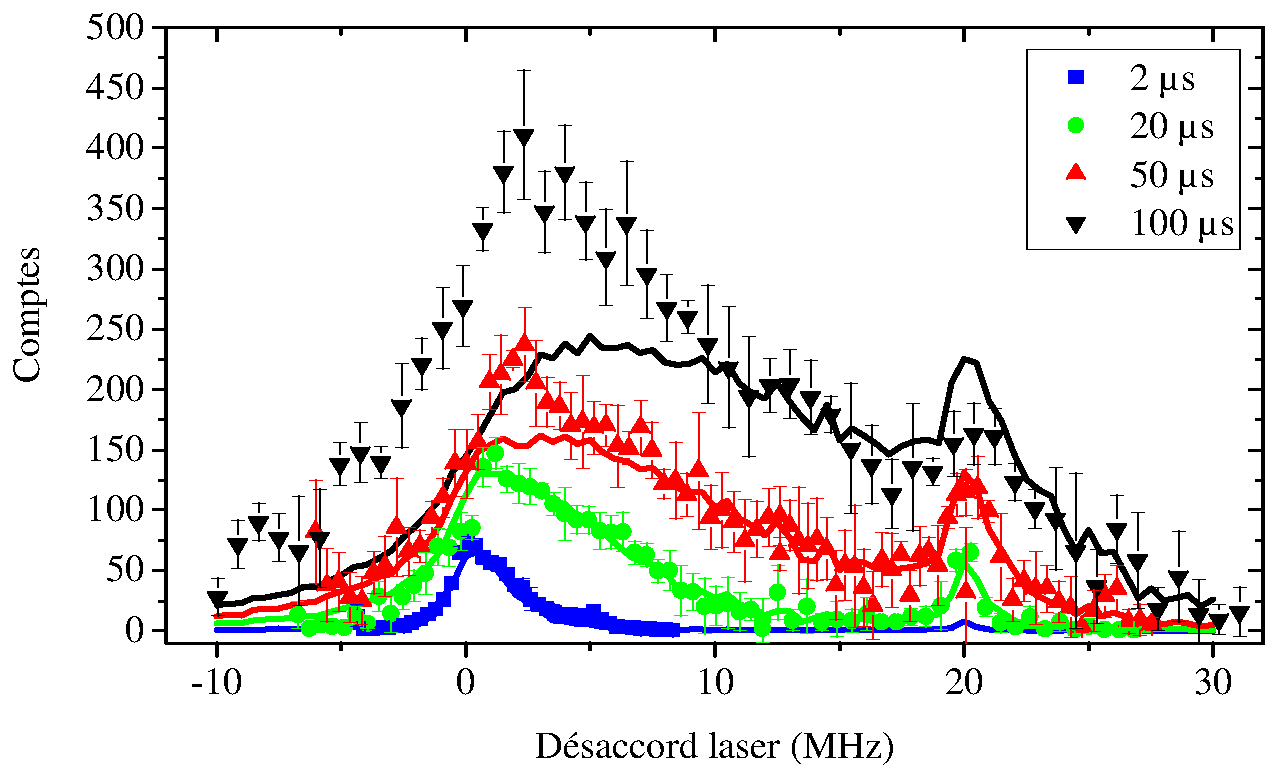
\includegraphics[width=\linewidth]{figures/low_l/fitsim_spectresoptiques_fin}
\caption[Comparaison des spectres optiques aux simulations avec équations de taux]{
Comparaison des spectres optiques aux simulations, pour différentes durées d'impulsion laser : $\SI{2}{},\SI{20}{},\SI{50}{}$ et $\SI{100}{\us}$.
Les spectres expérimentaux sont ceux de la figure \ref{fig:data_spectresoptiques}.
Les lignes pleines sont les résultats de la simulation.
Le calcul tient compte du mouvement des atomes de Rydberg durant l'excitation et des processus aléatoires d'absorption et ré-émission de photons rouges par les atomes dans l'état fondamental.
%Les traits pointillés sont les résultats des simulations sans tenir compte de l'effet de chauffage du nuage atomique.
}
\label{fig:fitsim_spectresoptiques_fin}
\end{figure}

\begin{table}[!h]
	\centering
	\caption[Paramètres de simulation]{Valeurs expérimentales et de simulation des paramètres d'excitation des spectres.
	}
	\label{tab:fit_sim_finalparam}
	\begin{tabular}{l c c}
		\toprule\midrule
		Paramètres fixes &	Valeur expérimentale & Valeur de simulation\\		
		\midrule
		Fréquence de piégeage $f_x$ & \SI{47}{\Hz} & \SI{47}{\Hz} \\
		Fréquence de piégeage $f_y$ & \SI{244}{\Hz} & \SI{244}{\Hz} \\
		Fréquence de piégeage $f_z$ & \SI{262}{\Hz} & \SI{262}{\Hz} \\
		Nombre d'atomes $N$ & $\SI{12000}{}\pm\SI{2000}{}$ & $\SI{12000}{}\pm\SI{2000}{}$ \\
		Col du laser bleu $w_{480}$ & \SI{22}{\um} & \SI{22}{\um} \\
		Col du laser rouge $w_{780}$ & \SI{150}{\um} & $\infty$ \\
		Largeur de raie $\gamma$ & \SI{626}{\kHz} & \SI{626}{\kHz}\\
		Taux ém. spont. photons rouges $\Gamma_{sp}$ & $2\pi\times\SI{16.6}{\kHz}$ & $2\pi\times\SI{16.6}{\kHz}$ \\
		\midrule
		Paramètres d'ajustement & &\\\midrule
		Amplitude de bande latérale $x_{20}$ & non mesurée & \SI{0.12}{} \\
		Fréquence de Rabi max. $\Omega_0/(2\pi)$ & \SI{296}{\kHz} & $\SI{60}{} \pm \SI{5}{\kHz}$\\
		Température initiale $T_0$ & $\SI{0.6}{}\pm\SI{0.3}{\uK}$ & $\SI{0.8}{}\pm\SI{0.05}{\uK}$\\
		\midrule
		\bottomrule
 	\end{tabular}
\end{table}



\clearpage
\subsection{Caractéristiques des nuages simulés}
\noindent Le très bon accord aux temps courts entre les simulations et les données expérimentales nous autorise à déduire des simulations certaines caractéristiques des nuages d'atomes de Rydberg excités par laser.
En particulier, nous nous intéressons ici à la distribution spatiale des atomes de Rydberg, ainsi qu'à la dynamique d'excitation aux temps courts.

\subsubsection*{Distribution radiale des nuages de Rydberg}
\noindent La distribution spatiale des atomes de Rydberg excités dans un nuage peut être représentée par sa fonction de distribution radiale $g^{(2)}(r)$.
Cette fonction décompte le nombre de paires d'atomes séparées d'une distance $r$ au sein d'un ensemble donné.
Ici, nous la définissons comme
\begin{equation}
\label{eq:g2r_def}
g^{(2)}(r) = \frac{1}{N(N-1)} \sum_{\langle i,j \rangle}{\delta (r-r_{ij})},
\end{equation}
où $N$ est le nombre d'atomes de l'ensemble et où la somme est faite sur les $N(N-1)$ paires $\langle i,j \rangle$ d'atomes.
Les figures \ref{fig:spatial_distrib_sim} a) et c) représentent cette fonction $g^{(2)}(r)$ pour des nuages de Rydberg excités avec différents désaccords, pendant des durées de $\SI{2}{}$ et $\SI{20}{\us}$ respectivement.

Il est d'usage de comparer la fonction de distribution radiale d'un ensemble à un cas idéal.
Ce cas idéal est généralement celui du gaz parfait lorsque l'on s'intéresse à l'agencement de particules classiques dans un ensemble thermodynamique.
Il est plus pertinent ici de comparer les distributions radiales des nuages de Rydberg à celle du nuage d'atomes dans l'état fondamental, notée $g^{(2)}_{~0}$.
Les distributions radiales normalisées $g^{(2)}(r)/g^{(2)}_{~0}(r)$ des nuages de Rydberg excités avec différents désaccords et pendant des durées de $\SI{2}{}$ et $\SI{20}{\us}$ sont représentées en figures \ref{fig:spatial_distrib_sim} b) et d) respectivement.

Les fonctions de distribution radiale montrent très clairement les effets de blocage dipolaire et de facilitation.
En effet, il n'y a jamais deux atomes de Rydberg excités à des distances inférieures au rayon de blocage $r_b=\sqrt[6]{2C_6/\gamma}$ (pour l'excitation à résonance) ou au rayon de facilitation $r_f=\sqrt[6]{C_6/\Delta}$ (pour l'excitation désaccordée), définis en \ref{subsec:excitation_bloc_facil}.

Les fonctions de distribution radiale montrent également la saturation du nuage : l'ensemble d'atomes de Rydberg excité pendant $\SI{2}{\us}$ à résonance s'étend bien au-delà du nuage d'atomes dans l'état fondamental.
En effet, le centre du nuage gaussien d'atomes dans l'état fondamental est vite saturé d'atomes de Rydberg en raison du blocage dipolaire, et les atomes de Rydberg supplémentaires doivent être excités loin du centre, dans les ailes peu denses du nuage.

Cette saturation se retrouve aussi pour l'excitation facilitée à désaccord positif si l'impulsion laser dure suffisamment longtemps.
L'extension d'un ensemble d'atomes de Rydberg excité à $\SI{2}{\MHz}$
est plus petite que celle du nuage d'atomes dans l'état fondamental pour une durée d'impulsion de $\SI{2}{\us}$, mais plus grande pour une durée d'impulsion de $\SI{20}{\us}$.
L'ensemble d'atomes de Rydberg excité à $\Delta=\SI{4}{\MHz}$ montre lui aussi une telle saturation, mais de façon moins importante : il faudra attendre plus longtemps pour exciter des atomes de Rydberg loin dans les ailes du nuage.
En effet, plus le désaccord laser est important, plus il faut de temps avant d'exciter un  permier atome de Rydberg (une \og graine \fg{}) et plus l'agrégat de Rydberg créé est compact car le rayon de facilitation est plus petit.

\begin{figure}[h]
\centering
%fonctions de corrélation de paire
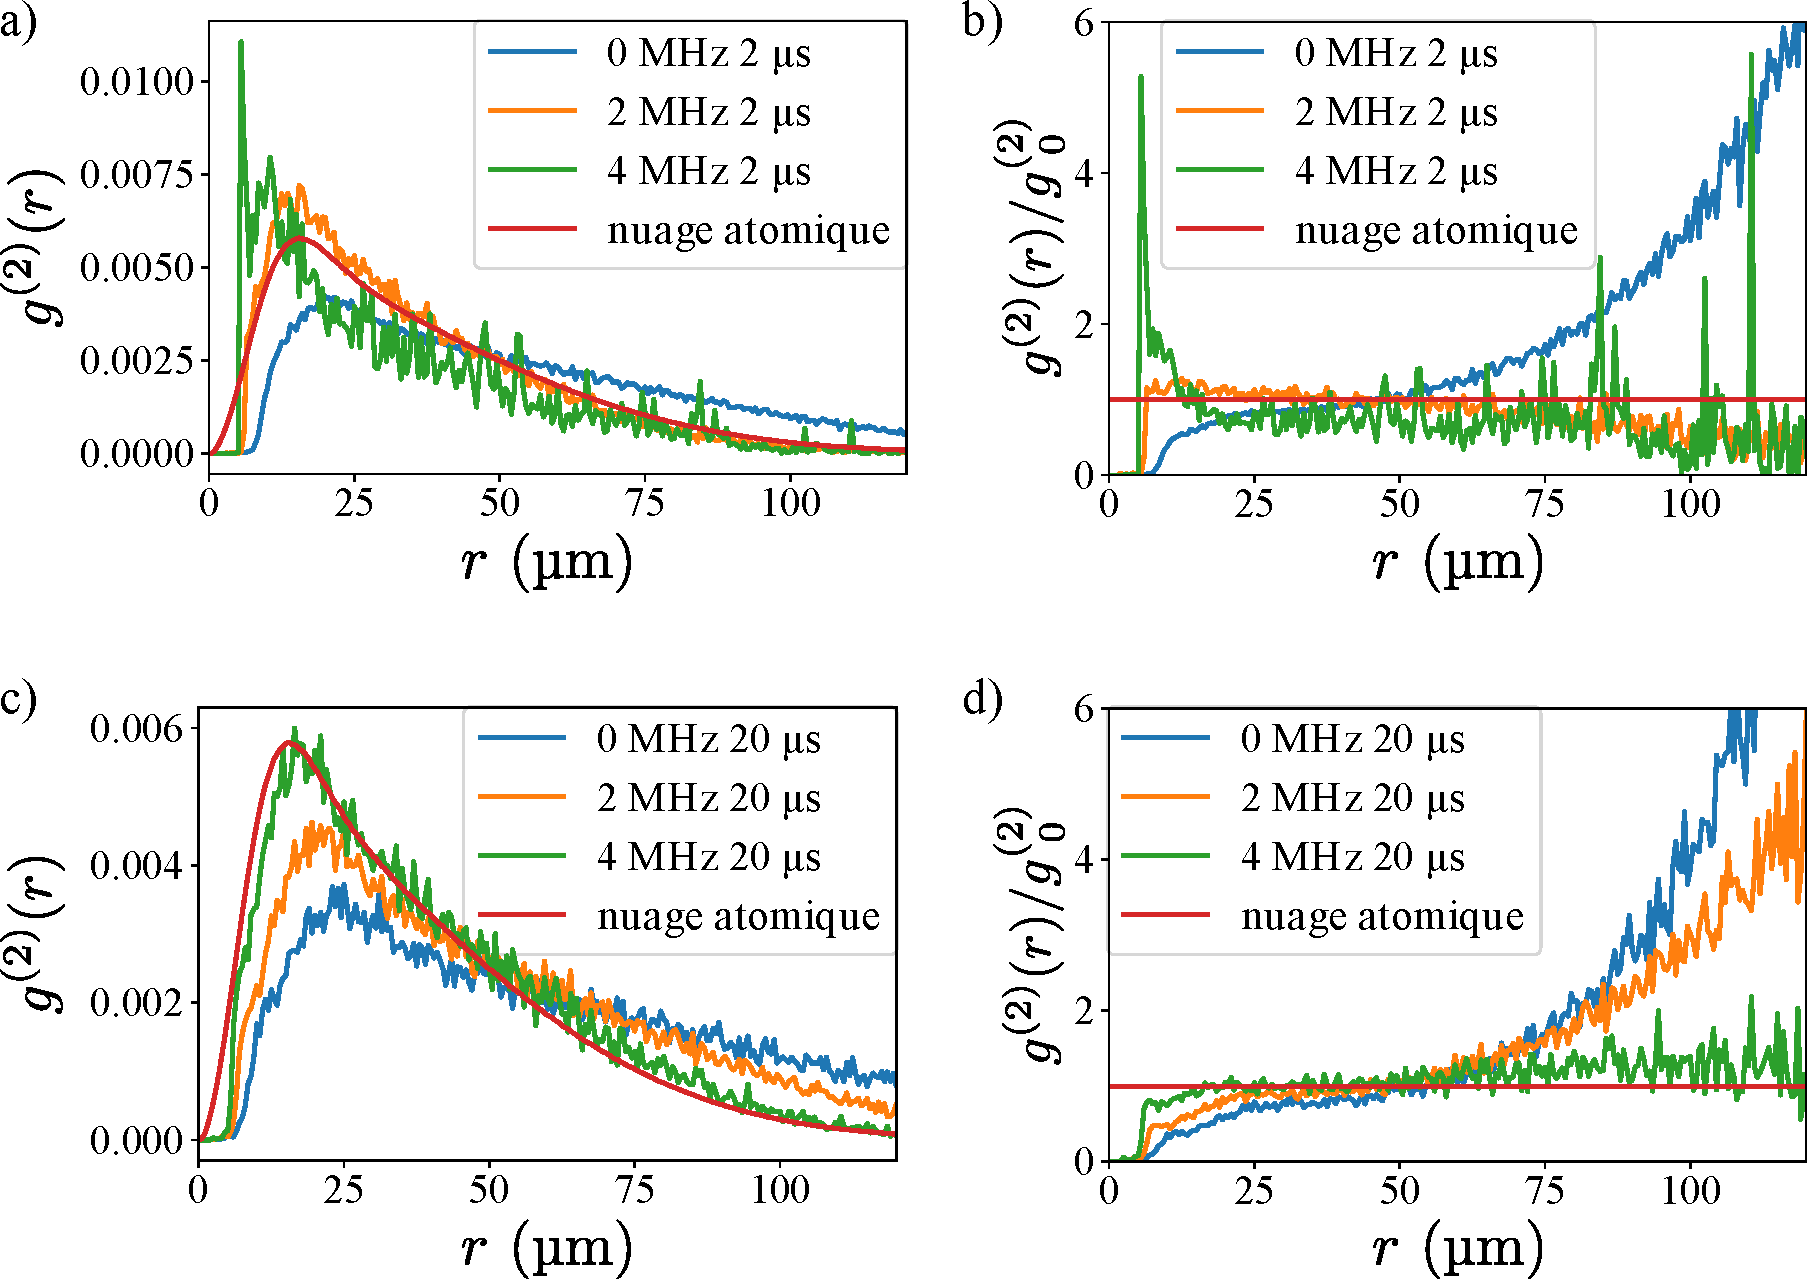
\includegraphics[width=\linewidth]{figures/low_l/g2r_all}
%distribution spatiale à résonance et à 2MHz, image2D + "gaussienne" selon une direction\\
%pour $\SI{2}{\us}$
\caption[Distribution radiale des nuages de Rydberg simulés]{
Distribution radiale des nuages de Rydberg simulés.
Les courbes représentent les fonctions $g^{(2)}(r)$ (\textbf{a} et \textbf{c}) et $g^{(2)}(r)/g^{(2)}_{~0}(r)$ (\textbf{b} et \textbf{d}) pour des nuages de Rydberg excités à différents désaccords : à résonance (bleu), à $\SI{2}{\MHz}$ (orange) et à $\SI{4}{\MHz}$ (vert).
Les courbes rouges en trait pointillé représentent la fonction de distribution radiale $g^{(2)}_{~0}$ du nuage d'atomes froids dans l'état fondamental.
Les graphes \textbf{a)} et \textbf{b)} présentent les résultats pour un durée d'impulsion laser de $\SI{2}{\us}$ et les graphes \textbf{c)} et \textbf{d)} pour une durée d'impulsion laser de $\SI{20}{\us}$.
Les résultats sont moyennés sur $100$ réalisations lorsque la durée d'impulsion est de $\SI{2}{\us}$ et sur $5$ réalisations lorsque la durée d'impulsion est de $\SI{20}{\us}$.
}
\label{fig:spatial_distrib_sim}
\end{figure}
%
%

\clearpage
\subsubsection*{Dynamique d'excitation aux temps courts}
\noindent L'observation de la dynamique d'excitation aux temps courts permet également de mettre en évidence une saturation.
La figure \eqref{fig:satur_optical_sim} représente l'évolution simulée du nombre  d'atomes de Rydberg excités en fonction de la durée d'impulsion laser pour différents désaccords.% : $\SI{0}{},\SI{2}{},\SI{4}{}$ et $\SI{8}{\MHz}$.

Lorsque le laser est à résonance, le nombre d'atomes de Rydberg croît très vite jusqu'à $\SI{1.5}{\us}$.
Au-delà de cette durée, le nombre d'atomes de Rydberg croît de moins en moins rapidement.
Le nombre d'atomes de Rydberg ne sature cependant pas, en raison de la présence d'atomes disponibles pour être excités dans les ailes peu denses du nuage d'atomes dans l'état fondamental et en raison du chauffage de ce nuage, qui fait croître son extension au cours du temps.
Cette croissance rend sans cesse de nouveaux atomes dans l'état fondamental disponibles pour être excités, en les éloignant des atomes de Rydberg déjà excités.

Lorsque le laser est désaccordé, la croissance initiale du nombre d'atomes de Rydberg est plus lente.
En effet, le désaccord du laser rend l'excitation du premier atome de Rydberg plus tardive.
Le taux de croissance du nombre d'atomes de Rydberg dépend ensuite de la densité d'atomes dans l'état fondamental et de la largeur du laser : plus la densité est élevée et plus le laser est large, plus il y a d'atomes disponibles pour être excités dans la région de facilitation.
Or, plus le désaccord laser est important, plus le volume de cette région de facilitation est petit.
La croissance du nombre d'atomes de Rydberg excités est donc plus lente lorsque le désaccord laser augmente, même après excitation de la graine.

\begin{figure}[h]
\centering
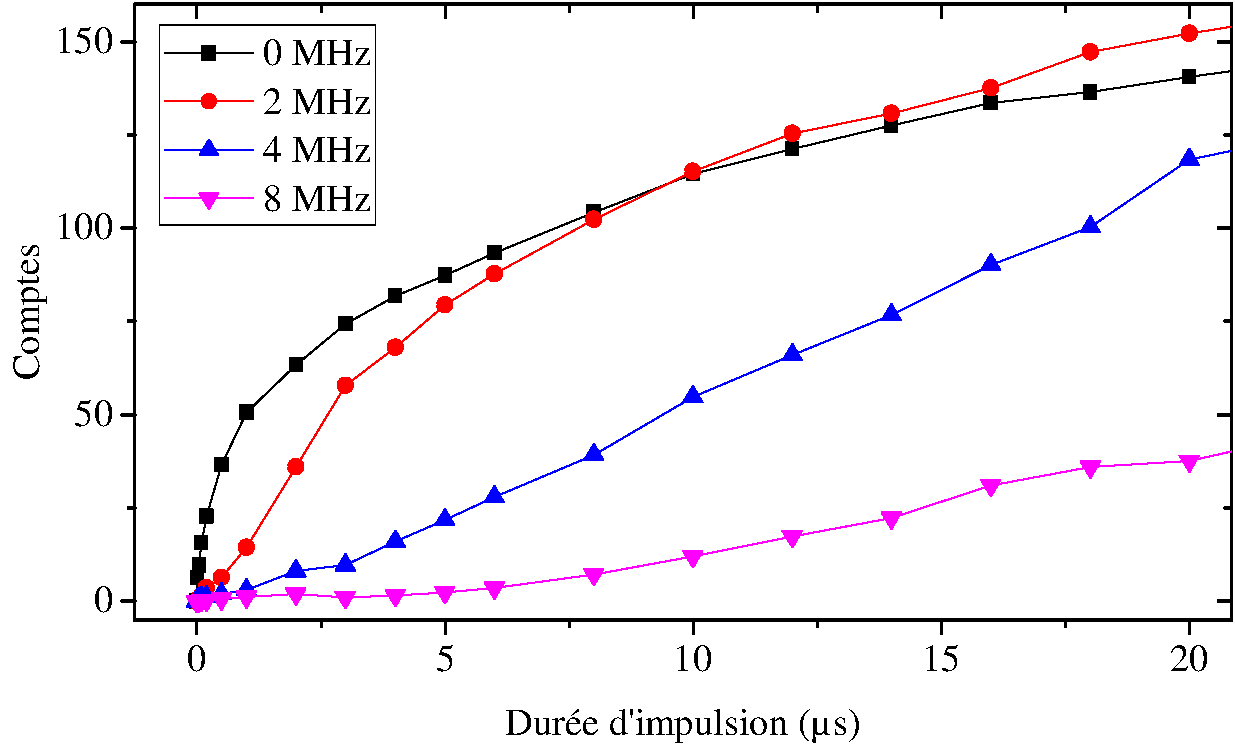
\includegraphics[width=\linewidth]{figures/low_l/satur_optical_sim}
\caption[\'Evolution simulée du nombre d'atomes de Rydberg excités en fonction du temps pour différents désaccords laser]{
\'Evolution simulée du nombre d'atomes de Rydberg excités en fonction du temps, pour différents désaccords laser : $\SI{0}{},\SI{2}{},\SI{4}{}$ et $\SI{8}{\MHz}$, tracés en noir, rouge, bleu et magenta respectivement.
Les points sont les données extraites de simulations moyennées sur $\SI{5}{}$ réalisations. Les lignes qui les relient servent de guides visuels.
}
\label{fig:satur_optical_sim}
\end{figure}

\clearpage
\section*{Conclusion}
\noindent Dans ce chapitre, nous avons discuté de l'influence des interactions sur l'excitation d'un ensemble d'atomes de Rydberg.
Les interactions dipôle-dipôle entre atomes de Rydberg sont responsables du blocage dipolaire, qui interdit l'excitation d'un second atome de Rydberg à proximité d'un premier.
Avec un laser désaccordé vers le bleu, l'excitation passe d'un régime de blocage dipolaire à un régime d'excitation facilitée : le désaccord du laser permet d'exciter de nouveaux atomes de Rydberg autour d'un premier, dans la région de l'espace où les interactions dipôle-dipôle et le désaccord du laser sont suffisamment proches.
Enfin, les interactions répulsives entre atomes de Rydberg causent l'expansion mécanique de l'ensemble d'atomes de Rydberg déjà excités.

Les effets de blocage dipolaire et d'excitation facilitée sont mis en évidence par la saturation et l'élargissement des spectres d'excitation optique lorsque la durée de l'impulsion laser augmente.
L'expansion mécanique du nuage d'atomes de Rydberg est mise en évidence par la spectroscopie microonde de la transition $\mathrm{60S}\rightarrow\mathrm{57S}$.
Le spectre de cette transition révèle directement le spectre des énergies d'interaction au sein de l'ensemble d'atomes de Rydberg.
L'évolution de ce spectre des énergies d'interaction après l'excitation des atomes de Rydberg montre en particulier que l'approximation du gaz gelé, consistant à s'intéresser aux interactions entre atomes de Rydberg en considérant que ceux-ci sont immobiles, ne peut être justifiée qu'aux temps très courts, de l'ordre de $\SI{10}{\us}$.

Afin de vérifier notre compréhension de la dynamique d'excitation et d'expansion des ensembles denses d'atomes de Rydberg, nous avons mis en \oe uvre des simulations numériques.
Un premier modèle Monte-Carlo, fondé sur le tirage au sort d'atomes dans l'état fondamental au sein du nuage, montre un accord qualitatif correct aux temps d'excitation courts.
Cela permet d'en extraire des conditions initiales pour simuler le mouvement de l'ensemble d'atomes de Rydberg après excitation, et comparer les résultats du modèle avec les données expérimentales de spectroscopie microonde.
L'accord est ici bon.

Ce premier modèle est cependant incapable de reproduire les spectres d'excitation optiques avec des durées d'impulsion laser longues, et ne présente qu'un accord qualitatif aux temps courts.
Nous avons donc développé un second modèle numérique, fondé sur des équations de taux issues des équations de Bloch optiques et calculées pour chaque atome, qu'il soit dans l'état fondamental ou dans un état de Rydberg, à chaque pas de temps.
L'introduction d'une échelle de temps lors de l'excitation des atomes de Rydbderg permet de prendre en compte directement leur mouvement, dû aux interactions dipôle-dipôle, pendant la phase d'excitation.

%De plus, nous avons ajouté à ce modèle le chauffage du nuage d'atomes dans l'état fondamental dû au laser rouge d'excitation, et qui est responsable de l'accroissement de la taille de ce nuage au cours du temps.
%%
%%Grâce à ce modèle, nous avons pu reproduire les spectres d'excitation optique à temps long.
%%La figure \eqref{fig:sim_nomvt_noheat} montre l'importance de prendre en compte le mouvement des atomes de Rydberg et le chauffage du nuage atomique pendant l'excitation.
%%En particulier, l'approximation du gaz gelé, consistant à s'intéresser aux interactions entre atomes de Rydberg en considérant que ceux-ci sont immobiles, ne peut être justifiée qu'aux temps très courts, de l'ordre de $\SI{10}{\us}$.
%%
%%
%Ce modèle permet de mieux reproduire les spectres à temps courts, voire même jusqu'à $\SI{50}{\us}$ de durée d'impulsion laser, mais n'est pas suffisant pour rendre compte du spectre laser à $\SI{100}{\us}$ d'impulsion.
%\begin{figure}[!h]
%\centering
%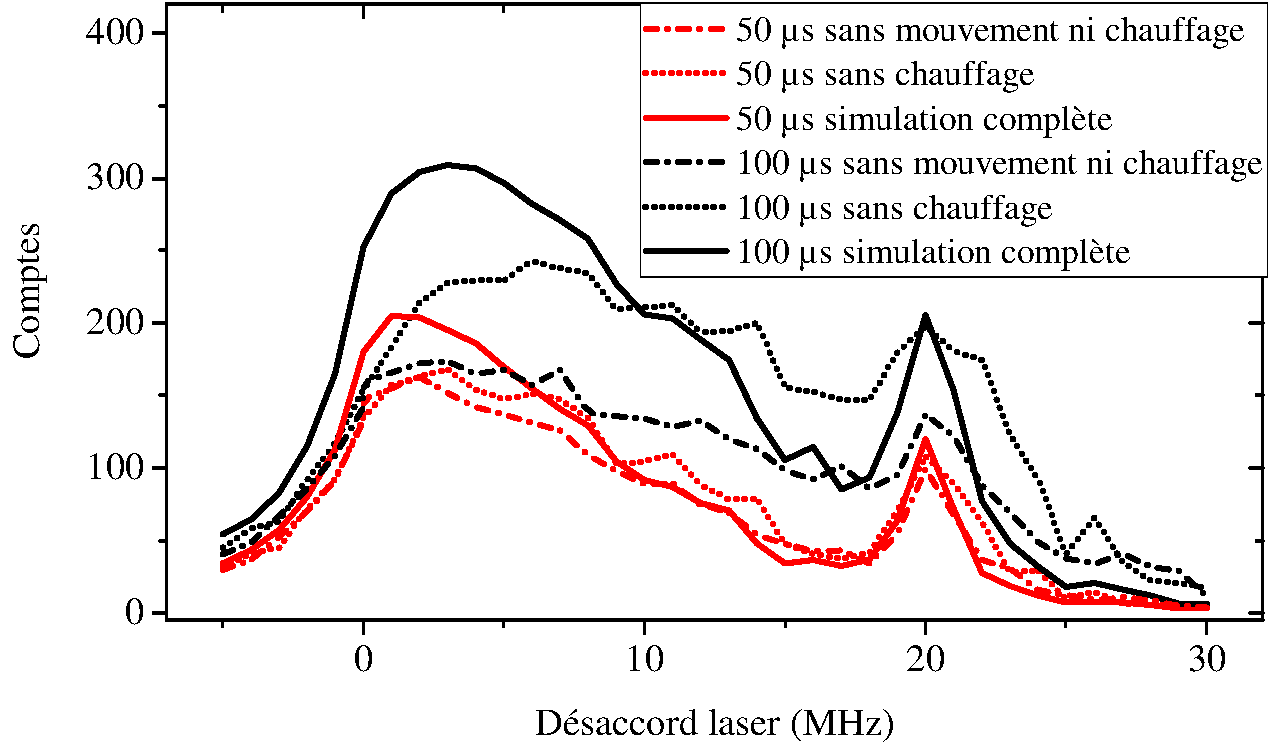
\includegraphics[width=\linewidth]{figures/low_l/sim_nomvt_noheat}
%%Résultats des simulations, 1.avec mvt et chauffage, 2. sans mvt, 3. sans chauffage.
%\caption[Comparaison des différents effets pris en compte dans les simulations]{
%Comparaison des différents effets pris en compte dans les simulations, pour des durées d'impulsions laser de $\SI{50}{}$ (rouge) et $\SI{100}{\us}$ (noir).
%Les courbes en trait point-tiret représentent les résultats des simulations ne prenant en compte ni le mouvement des atomes de Rydberg par interaction répulsive, ni le chauffage des atomes dans l'état fondamental dû au laser rouge.
%Les courbes en pointillés représentent les résultats des simulations avec le mouvement des atomes de Rydberg mais sans chauffage du nuage atomique.
%Les courbes en trait plein représentent les résultats des simulations complètes, intégrant le mouvement des atomes de Rydberg et le chauffage du nuage atomique.
%\`A $\SI{50}{\us}$, l'effet du mouvement des atomes de Rydberg est assez faible mais l'effet du chauffage du nuage d'atomes dans l'état fondamental est déjà important.
%\`A $\SI{100}{\us}$, l'effet du mouvement des atomes de Rydberg devient lui aussi significatif.
%}
%\label{fig:sim_nomvt_noheat}
%\end{figure}
%
%\clearpage
%\newpage

Ce modèle permet de très bien reproduire les spectres expérimentaux, à condition d'inclure un processus d'expansion du nuage atomique pendant l'excitation.
Cependant, le chauffage du nuage dû au laser rouge d'excitation est largement insuffisant à expliquer une telle expansion.
En l'absence de phénomène pouvant l'expliquer, nous avons renoncé à intégrer cette expansion à notre modèle final.
Celui-ci reproduit encore très bien les spectres d'excitation avec des durées d'impulsion laser de $\SI{2}{}$ et $\SI{20}{\us}$, même s'il n'est pas satisfaisant pour les durées d'impulsion plus longues.
%Les simulations ne montrent qu'un accord qualitatif avec les spectres enregistrés avec des impulsions de $\SI{50}{}$ et $\SI{100}{\us}$ ne 

Enfin, le bon accord des simulations avec les données expérimentales aux temps courts nous autorise à extrapoler, à partir du modèle numérique, certaines propriétés de l'excitation des ensembles denses d'atomes de Rydberg.
L'évolution du nombre d'atomes de Rydberg dans les premiers temps de l'excitation montre un comportement de quasi-saturation du nuage, après quoi les atomes de Rydberg ne sont plus excités que dans les ailes peu denses du nuage atomique.
La fonction de distribution radiale des nuages ainsi excités confirme cet effet de saturation, et montre très clairement les effets de blocage dipolaire et d'excitation facilitée.